\documentclass[11pt]{report}

% Dependencies
\usepackage{graphicx}
\usepackage{amsmath}
\usepackage{multicol}
\usepackage{amssymb}
\usepackage{multirow}
\usepackage{cases}
\usepackage{tabularx}
\usepackage{xcolor}
\usepackage{fancyhdr}
\usepackage{fontspec}
\usepackage{titlesec, blindtext}
\usepackage[spanish,es-tabla]{babel}
\usepackage{tocloft}
\usepackage[
    hyperindex=true,
    bookmarks=true,
    bookmarksnumbered=true,
    hidelinks,
]{hyperref}
\usepackage[all]{hypcap}
\usepackage{caption}
\usepackage{subcaption}
\usepackage{float}
\usepackage{bytefield}
\usepackage{listings}
\lstset{
  basicstyle=\ttfamily\footnotesize,
  columns=fullflexible,
  numbers=left,
  frame=single,
  breaklines=true,
  postbreak=\mbox{\textcolor{red}{$\hookrightarrow$}\space},
}
\usepackage{tikz}
\usepackage{longtable}

%%%%%%%%%%%%%%%%%%%%%%%%%%%%%%%%%%%%%%%%%%%%%%%%%%%%%%%%%%%%%%%%%%%%%%%%%%%%%%%
% Document style                                                              %
%%%%%%%%%%%%%%%%%%%%%%%%%%%%%%%%%%%%%%%%%%%%%%%%%%%%%%%%%%%%%%%%%%%%%%%%%%%%%%%

\usepackage[
    lmargin=3cm,
    rmargin=3cm,
    tmargin=2.5cm,
    bmargin=2.5cm,
]{geometry}
\setmainfont{Arial}
\definecolor{greyed}{RGB}{242,242,242}

\fancypagestyle{plain}{
    \setlength{\headheight}{18.18pt}
    \fancyhf{}
    \fancyhead[L]{
        \color{gray}
        \scriptsize
        Desarrollo de una herramienta de análisis de tráfico de red y su uso en algoritmos de ML para la detección de ataques.
        \\
        Raul Rabadan Arroyo
    }
    %\renewcommand{\headrulewidth}{0pt}
    \fancyfoot[R]{\thepage}
}
\pagestyle{plain}

\fancypagestyle{nonumber}{
    \fancyhf{}
    \renewcommand{\headrulewidth}{0pt}
}

\titleformat{\chapter}[hang]{\huge\bfseries}{\theHchapter.~}{0pt}{\huge\bfseries}
\titlespacing*{\chapter}{0pt}{0pt}{12pt}

\renewcommand{\baselinestretch}{1.5} 

\bibliographystyle{unsrt}
\addto\captionsspanish{\renewcommand{\bibname}{BIBLIOGRAFÍA}}

%%%%%%%%%%%%%%%%%%%%%%%%%%%%%%%%%%%%%%%%%%%%%%%%%%%%%%%%%%%%%%%%%%%%%%%%%%%%%%%
% Table of contents style                                                     %
%%%%%%%%%%%%%%%%%%%%%%%%%%%%%%%%%%%%%%%%%%%%%%%%%%%%%%%%%%%%%%%%%%%%%%%%%%%%%%%

\tocloftpagestyle{empty}

% Table of contents title
\setlength{\cftbeforetoctitleskip}{0ex}%
\setlength{\cftaftertoctitleskip}{0ex}%
\renewcommand{\cfttoctitlefont}{\hfill\textbf}%
\renewcommand{\cftaftertoctitle}{\hfill}%
\addto\captionsspanish{\renewcommand{\contentsname}{ÍNDICE}}

% Table of contents chapter
\setlength{\cftbeforechapskip}{1em}%
\setlength{\cftchapindent}{0em}%
\renewcommand{\cftchapaftersnum}{. \space}%
\renewcommand{\cftchapleader}{\hfill}%

% Table of contents section
\setlength{\cftbeforesecskip}{0.5em}%
\setlength{\cftsecindent}{0em}%
\renewcommand{\cftsecfont}{\bfseries\footnotesize}%
\renewcommand{\cftsecpagefont}{\bfseries\footnotesize}%
\renewcommand{\cftsecaftersnum}{. \space}%
\renewcommand{\cftsecleader}{\hfill}%

% Table of contents subsection
\setlength{\cftbeforesubsecskip}{0.5em}%
\setlength{\cftsubsecindent}{0em}%
\renewcommand{\cftsubsecfont}{\bfseries\footnotesize}%
\renewcommand{\cftsubsecpagefont}{\bfseries\footnotesize}%
\renewcommand{\cftsubsecaftersnum}{. \space}%
\renewcommand{\cftsubsecleader}{\hfill}%

% Table of contents subsubsection
\setlength{\cftbeforesubsubsecskip}{0.5em}%
\setlength{\cftsubsubsecindent}{0em}%
\renewcommand{\cftsubsubsecfont}{\bfseries\footnotesize}%
\renewcommand{\cftsubsubsecpagefont}{\bfseries\footnotesize}%
\renewcommand{\cftsubsubsecaftersnum}{. \space}%
\renewcommand{\cftsubsubsecleader}{\hfill}%

% List of figures title
\setlength{\cftbeforeloftitleskip}{0ex}%
\setlength{\cftafterloftitleskip}{0ex}%
\renewcommand{\cftloftitlefont}{\hfill\textbf}%
\renewcommand{\cftafterloftitle}{\hfill}%
\addto\captionsspanish{\renewcommand{\listfigurename}{ÍNDICE DE FIGURAS}}

% List of figures point
\renewcommand{\cftfigleader}{\hfill}%
\setlength{\cftfignumwidth}{5em}
\renewcommand{\cftfigpresnum}{Figura~}
\renewcommand{\cftfigaftersnum}{.}

% List of tables title
\setlength{\cftbeforelottitleskip}{0ex}%
\setlength{\cftafterlottitleskip}{0ex}%
\renewcommand{\cftlottitlefont}{\hfill\textbf}%
\renewcommand{\cftafterlottitle}{\hfill}%
\addto\captionsspanish{\renewcommand{\listtablename}{ÍNDICE DE TABLAS}}

% List of tables point
\renewcommand{\cfttableader}{\hfill}%
\setlength{\cfttabnumwidth}{5em}
\renewcommand{\cfttabpresnum}{Tabla~}
\renewcommand{\cfttabaftersnum}{.}

%%%%%%%%%%%%%%%%%%%%%%%%%%%%%%%%%%%%%%%%%%%%%%%%%%%%%%%%%%%%%%%%%%%%%%%%%%%%%%%
% Glossary                                                                    %
%%%%%%%%%%%%%%%%%%%%%%%%%%%%%%%%%%%%%%%%%%%%%%%%%%%%%%%%%%%%%%%%%%%%%%%%%%%%%%%

% Import
\usepackage[acronym,automake,section=subsubsection]{glossaries}

% Generation
\makeglossaries

% Contents
\newglossaryentry{matrix}% the label
{name={matrix},% the term
 description={a rectangular table of elements},% brief description
 plural={matrices}% the plural
}

\newglossaryentry{userdatagramprotocol}% the label
{name={User Datagram Protocol},% the term
 description={Protocolo de red de la capa de transportes orientado a mensajes.},% brief description
}

\newacronym{ml}{ML}{Machine learning}
\newacronym{udp}{UDP}{User Datagram Protocol}

% Style

\addto\captionsspanish{\renewcommand{\glossaryname}{TÉRMINOS}}
\addto\captionsspanish{\renewcommand{\acronymname}{ACRÓNIMOS}}

%%%%%%%%%%%%%%%%%%%%%%%%%%%%%%%%%%%%%%%%%%%%%%%%%%%%%%%%%%%%%%%%%%%%%%%%%%%%%%%
% Document                                                                    %
%%%%%%%%%%%%%%%%%%%%%%%%%%%%%%%%%%%%%%%%%%%%%%%%%%%%%%%%%%%%%%%%%%%%%%%%%%%%%%%

\begin{document}

% Front pages
\selectlanguage{spanish}
\begin{titlepage}
    
\includegraphics{media/epsevg_logo.jpeg}
    \begin{center}

        \vspace{1.5cm}
        {\Huge\textbf{TRABAJO FINAL DE GRADO}}

        \vfill
        ~\\ % Empty line so its aligned to the appendices

        \vfill

        \setlength\fboxsep{0.5cm}\fbox{
            \parbox{13.5cm}{
                \par{
                    \textbf{TÍTULO:} \MakeUppercase[]{Desarrollo de una herramienta de análisis de tráfico de red y su uso en algoritmos de ML para la detección de ataques.}
                    \\[\baselineskip]
                    \textbf{AUTOR:} RABADAN ARROYO, RAUL
                    \\[\baselineskip]
                    \textbf{FECHA DE PRESENTACIÓN:} JULIO, 2024
                }
            }
        }

        \vfill

    \end{center}
\end{titlepage}

\begin{titlepage}
    \begin{center}
        \setlength\fboxsep{0.5cm}\fbox{
            \parbox{13.5cm}{
                \par{
                    \textbf{APELLIDOS:} RABADAN ARROYO \quad \textbf{NOMBRE:} RAUL \\[\baselineskip]
                    \textbf{TITULACIÓN:} GRADO EN INGENIERÍA INFORMÁTICA \\[\baselineskip]
                    \textbf{PLAN:} 2018 \\[\baselineskip]
                    \textbf{DIRECTORA:} SIMO MEZQUITA, ESTER \\[\baselineskip]
                    \textbf{DEPARTAMENTO:} DEPARTAMENTO DE MATEMÁTICAS
                }
            }
        }
    \end{center}
    
    \vfill

    \begin{center}
        \setlength\fboxsep{0cm}\colorbox{greyed}{\setlength\fboxsep{0.5cm}\fbox{
            \parbox[t]{7.5cm}{
                \centering{
                    \textbf{CALIFICACIÓN DEL TFG}
                }
                \vspace {
                    2cm
                }
            }
        }}
    \end{center}

    \vfill

    \begin{center}
        \setlength\fboxsep{0cm}\colorbox{greyed}{\setlength\fboxsep{0.5cm}\fbox{
            \parbox{13.5cm}{
                \begin{center}
                    \underline{
                        \textbf{
                            TRIBUNAL
                        }
                    }
                \end{center}
                
                \hspace{1cm}
                \textbf{PRESIDENTE}
                \hfill
                \textbf{SECRETARIO}
                \hfill
                ~~ % Make it the same with as the others
                \textbf{VOCAL}
                ~~~ % Make it the same with as the others
                \hspace{1.3cm}

                \vspace {
                    3cm
                }
                \hspace{0.9cm}
                \textbf{FECHA DE LECTURA:}
                \vspace {
                    0.5cm
                }
            }
        }}
    \end{center}

    \vfill

    \begin{center}
        \textbf{
            Este proyecto tiene en cuenta aspectos medioambientales: \square ~ Sí ~ \blacksquare ~ No
        }
    \end{center}
    
\end{titlepage}

% Abatracts
\selectlanguage{spanish}
\newpage
\pagestyle{nonumber}

\begin{center}
    \textbf{
        RESUMEN
    }
    \\[\baselineskip]
\end{center}

\begin{center}
    \setlength\fboxsep{0.05\textwidth}\fbox{
        \parbox[t][\textwidth]{0.8\textwidth}{
            \quad \quad En este trabajo se hace el desarrollo de una herramienta de análisis de red y se demuestra su funcionamiento a partir de analizar trazas de tráfico de red y su uso en algoritmos de Machine Learning.
            
            \quad \quad Para el desarrollo de la herramienta se ha hecho uso de Rust y en las tareas de Machine Learning y análisis de datos se ha trabajado con Python. El desarrollo se ha realizado bajo un entorno de desarrollo en un contenedor Docker. Todo el código de la herramienta, los scripts y la configuración del entorno se ofrecen para permitir resultados lo más reproducibles posibles.
            
            \quad \quad La herramienta es capaz de generar 72 características continuas con información de flujos TCP y UDP, además de 2 discretas indicando el protocolo de transporte y una identificación de cada flujo compuesta por 7 valores. Adicionalmente, la herramienta permite realizar un etiquetado automático a partir de un fichero CSV en el cual se indica por cada fila el par de direcciones IP, el protocolo de transporte utilizado y el tiempo de inicio y 
            final.
            
            \quad \quad A partir de los conjuntos de datos utilizados, la herramienta desarrollada y un modelo basado en bosques aleatorios, se ha obtenido un valor de precisión del 99.95\% y una puntuación F1 media del 98.66\%
            
            \quad \quad La herramienta desarrollada puede ser utilizada como componente en sistemas  de detección de intrusiones y tiene el potencial para ser extendida con más funcionalidades en el futuro.
        }
    }
\end{center}

\vspace{0.3cm}
\textbf{Palabras clave:}
\begin{center}
    \renewcommand{\arraystretch}{1.5}\begin{tabular}{|m{0.2\textwidth}|m{0.2\textwidth}|m{0.2\textwidth}|m{0.2\textwidth}|}
        \hline
            \centering\arraybackslash{Análisis de red} & \centering\arraybackslash{Machine Learning} & \centering\arraybackslash{Ciberseguridad} & \centering\arraybackslash{Desarrollo} \\
        \hline
        \centering\arraybackslash{Python} & \centering\arraybackslash{Rust} & \centering\arraybackslash{Docker} \\
        \cline{1-3}
    \end{tabular}
\end{center}

\selectlanguage{catalan}
\newpage
\pagestyle{nonumber}

\begin{center}
    \textbf{
        RESUM
    }
    \\[\baselineskip]
\end{center}

\begin{center}
    \setlength\fboxsep{0.05\textwidth}\fbox{
        \parbox[t][\textwidth]{0.8\textwidth}{
            \par{
                Amb una extensió màxima de 50 línies, i amb una llista de màxim 10 paraules clau, el resum és un text informatiu que permet decidir sobre la utilitat de llegir el document complet; ha de definir l’objectiu, els mètodes, els resultats i les conclusions presentats en el cos del document, en aquest ordre o destacant inicialment els resultats i les conclusions; ha de ser un text complet perquè sigui intel·ligible sense necessitat de referir-se a la memòria; ha de contenir la informació bàsica i el caràcter del document original. Com en tots els documents cal vetllar per la correcció d’estil, cal també emprar una nomenclatura normalitzada, i definir els termes no familiars les abreviacions i els símbols, quan apareguin per primera vegada en el resum. És la pàgina número 1 del document.
            }
        }
    }
\end{center}

\vspace{0.3cm}
\textbf{Paraules clau (màxim 10):}
\begin{center}
    \renewcommand{\arraystretch}{1.5}\begin{tabular}{|m{0.2\textwidth}|m{0.2\textwidth}|m{0.2\textwidth}|m{0.2\textwidth}|}
        \hline
            \centering\arraybackslash{?} & \centering\arraybackslash{?} & \centering\arraybackslash{?} & \centering\arraybackslash{?} \\
        \hline
        \centering\arraybackslash{?} & \centering\arraybackslash{?} & \centering\arraybackslash{?} & \centering\arraybackslash{?} \\
        \hline
        \centering\arraybackslash{?} & \centering\arraybackslash{?} \\
        \cline{1-2}
    \end{tabular}
\end{center}

\selectlanguage{english}
\newpage
\pagestyle{nonumber}

\begin{center}
    \textbf{
        ABSTRACT
    }
    \\[\baselineskip]
\end{center}

\begin{center}
    \setlength\fboxsep{0.05\textwidth}\fbox{
        \parbox[t][\textwidth]{0.8\textwidth}{
            \quad \quad This project contains the development of a network analysis tool, the showcase of its usage on network traces, and the employment of the results on Machine Learning algorithms.

            \quad \quad Rust has been used for the development of the tool and Python for the data analysis process and Machine Learning. The development has been made in a containerized development environment. All the code from the tool, the scripts and the configuration of the environment are available to allow for reproducible results.
            
            \quad \quad The tool is capable of generating 72 continuous features with information about the TCP and UDP flows. In addition to the previous, it adds 2 discrete columns to indicate the used protocol and 7 values to be able to identify each detected flow. Additionally, the tool allows the user to provide a \acrshort{csv} file in order to perform automatic tagging. This file should contain, for each record, the pair of IP addresses, the used transport protocol, and the starting and ending timestamps.
            
            \quad \quad With the source datasets, the developed tool and a model based on random forests, a precision value of 99.95\% and an average F1 macro score of 98.66\% were obtained.
            
            \quad \quad The tool can be used as a component in an intrusion detection system and has the possibility to be extended with more functionalities in the future.
        }
    }
\end{center}

\vspace{0.3cm}
\textbf{Keywords:}
\begin{center}
    \renewcommand{\arraystretch}{1.5}\begin{tabular}{|m{0.2\textwidth}|m{0.2\textwidth}|m{0.2\textwidth}|m{0.2\textwidth}|}
        \hline
            \centering\arraybackslash{Network analysis} & \centering\arraybackslash{Machine Learning} & \centering\arraybackslash{Cybersecurity} & \centering\arraybackslash{Development} \\
        \hline
        \centering\arraybackslash{Python} & \centering\arraybackslash{Rust} & \centering\arraybackslash{Docker} \\
        \cline{1-3}
    \end{tabular}
\end{center}


% Indices
\selectlanguage{spanish}
\selectlanguage{spanish}
\tableofcontents
\newpage
\listoffigures
\newpage
\listoftables
\newpage
\setglossarystyle{index}
%\hfill\textbf{GLOSARIO}\hfill
\printglossaries


% Contents
\newpage
\pagestyle{plain}

\phantomsection\addcontentsline{toc}{chapter}{INTRODUCCIÓN}
\chapter*{INTRODUCCIÓN}

La ciberseguridad es una de las fronteras del conocimiento que ha tomado más relevancia estos últimos años. Para salvaguardar la disponibilidad, integridad y confidencialidad de la información tanto almacenada como en tránsito, se aplican numerosas y diversas técnicas en conjunto. Desde medidas criptográficas para proteger la información hasta el análisis del tráfico de red para detectar comportamientos maliciosos y poder bloquearlos. El presente trabajo se focalizará en el último punto.

\phantomsection\addcontentsline{toc}{section}{MOTIVACIÓN}
\section*{MOTIVACIÓN}

La motivación de este trabajo radica en mi interés por la aplicabilidad de los sistemas de \gls{ml} en entornos limitados o con requerimientos de actuación en tiempo real, especialmente en el ámbito de ciberseguridad en las redes. En muchos casos, los tráficos de red maliciosos son identificados cuando estos ya han ocurrido o están generando problemas activamente para el resto de usuarios de la red La hazaña intelectual que supondría la detección de ataques en su inicio o incluso antes de que ocurriesen es una meta en la que me gustaría colaborar. Llegar a este ideal es seguramente improbable. Sin embargo, tenerlo como horizonte para dirigir el camino y acercarse lo máximo posible a este, ofrece la capacidad de mejorar la mitigación contra posibles adversarios.

Existen diversas herramientas similares a la ideada para el trabajo, pero debido a su dificultad de uso, su naturaleza propietaria o su desalineación al uso específico que se le quiere dar, he querido desarrollar una alternativa.

\phantomsection\addcontentsline{toc}{section}{OBJETIVOS}
\section*{OBJETIVOS}

El objetivo principal del trabajo consiste en diseñar, programar y demostrar la utilidad de una herramienta de análisis de red basada en la extracción de características de esta para detectar comportamientos maliciosos. La herramienta requerirá de ser robusta y eficiente, además de fácil de utilizar, extender y modificar. La robusteza y eficiencia son necesarias, ya que por su naturaleza tendrá que tratar datos en tiempo real en entornos limitados. La facilidad de uso, extensión y modificación es importante, ya que en el desarrollo de aplicaciones, y especialmente en el ámbito de la ciberseguridad, el entorno y los requerimientos están en constante variación.

La utilidad de la herramienta se evaluará según su capacidad de adaptación a diferentes entornos de ejecución y diferentes tipos de tráfico de red. Esto es necesario, ya que, dependiendo de su rendimiento, podrá ser integrada en sistemas más generales y complejos.

\phantomsection\addcontentsline{toc}{section}{METODOLOGÍA}
\section*{METODOLOGÍA}

(extreme programming, definir tests y metas etc)
\newpage
\pagestyle{plain}

\chapter{MARCO TEÓRICO}

\section{Anàlisis herramientas de extracción de características}

\subsection{CICFlowmeter}

CICFlowMeter es una herramienta para generar y analizar flujos de red \cite{cicflowpost}. Permite obtener información sobre flujos bidireccionales sobre IP, utilizen estos TCP o UDP. Por cada flujo, genera seis columnas identificativas y añade cierta información del flujo. En el Readme del codigo fuente ofrecido, podemos encontrar las características generades.

\begin{itemize}
    \item \textbf{Flow ID}: Combinación de las otras columnas separadas por giones
    \item \textbf{Src IP}: La dirección IP del remitente des de la cual se ha iniciado el flujo
    \item \textbf{Src Port}: La dirección IP del destinatario hacia la cual se ha dirigido el flujo
    \item \textbf{Dst IP}: El puerto origen o de retorno del remitente
    \item \textbf{Dst Port}: El puerto destino del destinatario
    \item \textbf{Protocol}: Identificador del protocolo sobre IP segun definido por IANA \cite{ipprotocolnumbers}
    \item \textbf{Timestamp}: Momento del incio del flujo, expresado en dd/MM/yyyy hh:mm:ss de la zona horaria local. En la descripción se indica que 
    \item \textbf{Flow Duration}: Duracion del flujo, expresado en microsegundos
    \item \textbf{Total Fwd Packet}: Número total de paquetes hacia el destinatario
    \item \textbf{Total Bwd packets}: Número total del paquetes hacia el receptor
    \item \textbf{Total Length of Fwd Packet}: Número completo de bytes transmitidos hacia el destinatario
    \item \textbf{Total Length of Bwd Packet}: Número completo de bytes recibidos des del destinatario
    \item \textbf{Fwd Packet Length Max}: Tamaño en bytes del paquete mas grande enviado hacia el destinatario
    \item \textbf{Fwd Packet Length Min}: Tamaño en bytes del paquete mas pequeño enviado hacia el destinatario
    \item \textbf{Fwd Packet Length Mean}: Media aritmética del tamaño en bytes de los paquetes enviados hacia el destinatario
    \item \textbf{Fwd Packet Length Std}: Desviación estándard del tamaño en bytes de los paquetes enviados hacia el destinatario
    \item \textbf{Bwd Packet Length Max}: Tamaño en bytes del paquete mas grande enviado hacia el emisor
    \item \textbf{Bwd Packet Length Min}: Tamaño en bytes del paquete mas pequeño enviado hacia el emisor
    \item \textbf{Bwd Packet Length Mean}: Media aritmética del tamaño en bytes de los paquetes enviados hacia el emisor
    \item \textbf{Bwd Packet Length Std}: Desviación estándard del tamaño en bytes de los paquetes enviados hacia el emisor
    \item \textbf{Flow Bytes s}: Bytes por segundo del flujo
    \item \textbf{Flow Packets s}: Paquetes por segundo del flujo
    \item \textbf{Flow IAT Mean}: Media aritmética del tiempo de llegada entre paquetes
    \item \textbf{Flow IAT Std}: Desviación estándard del tiempo de llegada entre paquetes
    \item \textbf{Flow IAT Max}: Tiempo máximo de llegada entre paquetes
    \item \textbf{Flow IAT Min}: Tiempo mínimo de llegada entre paquetes
    \item \textbf{Fwd IAT Total}: Tiempo total entre la llegada de dos paquetes hacia el receptor
    \item \textbf{Fwd IAT Mean}: Media aritmética del tiempo de llegada entre paquetes hacia el receptor
    \item \textbf{Fwd IAT Std}: Desviación estándard del tiempo de llegada entre paquetes hacia el receptor
    \item \textbf{Fwd IAT Max}: Tiempo máximo de llegada entre paquetes hacia el receptor
    \item \textbf{Fwd IAT Min}: Tiempo mínimo de llegada entre paquetes hacia el receptor
    \item \textbf{Bwd IAT Total}: Tiempo total entre la llegada de dos paquetes hacia el emisor
    \item \textbf{Bwd IAT Mean}: Media aritmética del tiempo de llegada entre paquetes hacia el emisor
    \item \textbf{Bwd IAT Std}: Desviación estándard del tiempo de llegada entre paquetes hacia el emisor
    \item \textbf{Bwd IAT Max}: Tiempo máximo de llegada entre paquetes hacia el emisor
    \item \textbf{Bwd IAT Min}: Tiempo mínimo de llegada entre paquetes hacia el emisor
    \item \textbf{Fwd PSH Flags}: Número de paquetes con el flag PSH activado en la cabecera TCP hacia el emisor
    \item \textbf{Bwd PSH Flags}: Número de paquetes con el flag PSH activado en la cabecera TCP hacia el receptor
    \item \textbf{Fwd URG Flags}: Número de paquetes con el flag URG activado en la cabecera TCP hacia el emisor
    \item \textbf{Bwd URG Flags}: Número de paquetes con el flag URG activado en la cabecera TCP hacia el receptor
    \item \textbf{Fwd Header Length}: Número de paquetes con el flag PSH activado en la cabecera TCP hacia el emisor
    \item \textbf{Bwd Header Length}: Número de paquetes con el flag PSH activado en la cabecera TCP hacia el receptor
    \item \textbf{Fwd Packets s}: Paquetes por segundo hacia el receptor
    \item \textbf{Bwd Packets s}: Paquetes por segundo hacia el emisor
    \item \textbf{Packet Length Min}: todo
    \item \textbf{Packet Length Max}: todo
    \item \textbf{Packet Length Mean}: todo
    \item \textbf{Packet Length Std}: todo
    \item \textbf{Packet Length Variance}: todo
    \item \textbf{FIN Flag Count}: todo
    \item \textbf{SYN Flag Count}: todo
    \item \textbf{RST Flag Count}: todo
    \item \textbf{PSH Flag Count}: todo
    \item \textbf{ACK Flag Count}: todo
    \item \textbf{URG Flag Count}: todo
    \item \textbf{CWR Flag Count}: todo
    \item \textbf{ECE Flag Count}: todo
    \item \textbf{Down Up Ratio}: todo
    \item \textbf{Average Packet Size}: todo
    \item \textbf{Fwd Segment Size.Avg}: todo
    \item \textbf{Bwd Segment Size Avg}: todo
    \item \textbf{Fwd Bytes Bulk Avg}: todo
    \item \textbf{Fwd Packet Bulk Avg}: todo
    \item \textbf{Fwd Bulk Rate Avg}: todo
    \item \textbf{Bwd Bytes Bulk Avg}: todo
    \item \textbf{Bwd Packet Bulk Avg}: todo
    \item \textbf{Bwd Bulk Rate Avg}: todo
    \item \textbf{Subflow Fwd Packets}: todo
    \item \textbf{Subflow Fwd Bytes}: todo
    \item \textbf{Subflow Bwd Packets}: todo
    \item \textbf{Subflow Bwd Bytes}: todo
    \item \textbf{FWD Init Win Bytes}: todo
    \item \textbf{Bwd Init Win Bytes}: todo
    \item \textbf{Fwd Act Data Pkts}: todo
    \item \textbf{Fwd Seg Size Min}: todo
    \item \textbf{Active Mean}: todo
    \item \textbf{Active Std}: todo
    \item \textbf{Active Max}: todo
    \item \textbf{Active Min}: todo
    \item \textbf{Idle Mean}: todo
    \item \textbf{Idle Std}: todo
    \item \textbf{Idle Max}: todo
    \item \textbf{Idle Min}: todo
\end{itemize}

\subsection{Wireshark}

a

\subsection{Zeek}

a

\subsection{ntopng}

a

\subsection{Argus}

a

\subsection{Softflowd}

a

\section{Datasets disponibles}

En esta sección analizaremos cuatro datasets disponibles utilizados para aplicaciones de ciberseguridad basadas en inteligencia artificial. Concretamente, observaremos CIC-DDos\-2019 \cite{8888419}, BoT-IoT \cite{DBLP:journals/corr/abs-1811-00701} \cite{10.1007/978-3-319-90775-8_3} \cite{KORONIOTIS202091} \cite{DBLP:journals/corr/abs-2005-00722} \cite{9252856} \cite{phdbotiot}, TON-IoT \cite{MOUSTAFA2021102994} \cite{9444348} \cite{9189760} \cite{9343133} \cite{9343084} \cite{moustafa2019systemic} \cite{ASHRAF2021103041} y UNSW-NB15 \cite{7348942} \cite{doi:10.1080/19393555.2015.1125974} \cite{7948715} \cite{Moustafa2017} \cite{10.1007/978-3-030-72802-1_9}.

\subsection{CICDDos2019}

\subsubsection{Descripción}

CICDDos2019 es un dataset creado por el Canadian Institute for Cybersecurity que contiene trazas de dos días en los que aparece tráfico benigno y serie de ataques DDoS típicos. \cite{cicddos2019web}. En este se contienen trazas de red en formato pcap y csvs con estadísticas de los flujos generados a partir de CICFlowMeter y posteriormente etiquetados. Para poder ofrecer un dataset público, realista y, además de mantener la privacidad de las comunicaciones originales, se generó tráfico sintético modelado a partir del comportamiento real de los usuarios. En las referencias se menciona el sistema utilizado para generar el comportamiento lo más natural posible de 25 usuarios haciendo uso de HTTP, HTTPS, FTP, SSH y protocolos de correo.

Los elementos de la red interna consisten en:

\begin{enumerate}
    \item Servidor web con Ubuntu 16.04 (192.168.50.1 en el primer día, 192.168.50.4 en el segundo día)
    \item Firewall con Fortinet (205.174.165.81)
    \item PC con Windows 7 (192.168.50.8 en el primer día, 192.168.50.9 en el segundo día)
    \item PC con Windows Vista (192.168.50.5 en el primer día, 192.168.50.6 en el segundo día)
    \item PC con Windows 8.1 (192.168.50.6 en el primer día, 192.168.50.7 en el segundo día)
    \item PC con Windows 10 (192.168.50.7 en el primer día, 192.168.50.8 en el segundo día)
\end{enumerate}

Adicionalmente, se han generado ataques DDoS basados en reflejos (usar un sistema de terceros para amplificar un ataque) y DDoS basado en exploits (tomar ventaja de vulnerabilidades en los protocolos). Según la información disponible \cite{cicddos2019web}, estos consisten en:

\begin{enumerate}
    \item \textbf{MSSQL}: Generado el primer día de 10:53 a 10:42 y el segundo de 11:36 a 11:45
    \item \textbf{SSDP}: Generado el segundo día de 12:27 a 12:37
    \item \textbf{DNS}: Generado el segundo día de 10:52 a 11:05
    \item \textbf{LDAP}: Generado el primer día de 10:21 a 10:30 y el segundo de 11:22 a 11:32
    \item \textbf{NetBIOS}: Generado el primer día de 10:00 a 10:09 y el segundo de 11:50 a 12:00
    \item \textbf{SNMP}: Generado el segundo día de 12:12 a 12:23
    \item \textbf{PortMap}: Generado el primer día de 9:43 a 9:51
    \item \textbf{WebDDoS}: Generado el segundo día de 13:18 a 13:29
    \item \textbf{NTP}: Generado el segundo día de 10:35 a 10:45
    \item \textbf{TFTP}: Generado el segundo día de 13:35 a 17:15
    \item \textbf{SYN Flood}: Generado el primer día de 11:28 a 17:35 y segundo día de 13:29 a 13:34
    \item \textbf{UDP Flood}: Generado el primer día de 10:53 a 11:03 y segundo día de 12:45 a 13:09
    \item \textbf{UDP-Lag}: Generado el primer día de 11:14 a 11:24 y segundo día de 13:11 a 13:15
\end{enumerate}

\subsubsection{Contenidos csvs}

El conjunto de datos procesados utilizando CICFlowMeter y etiquetado está compuesto por una lista de archivos por cada uno de los dos días en los que se generaron datos, el 3 de noviembre de 2018 y el 1 de diciembre de 2018. Las características ofrecidas son las mismas que las mencionadas en la herramienta CICFlowMeter. En todas las filas existen valores con excepción de algunas en la columna "Flow Bytes/s". Los scripts utilizados para la extracción y representación de los datos son \texttt{extract\_info\_cicddos\_2019.py} y \texttt{plot\_info\_cicddos\_2019.py} disponibles en TODO DEFINIR.

Como podemos ver en las figuras \ref{fig:cicddos_2019_csv_03-11_file_results} y \ref{fig:cicddos_2019_csv_01-12_file_results}, los archivos no contienen únicamente ataques etiquetados con su mismo nombre y benignos, sino que algunos contienen entre uno y dos adicionales. Para el primero, las categorías adicionales provienen de otros archivos. Para el segundo, la categoría adicional en UDPLag.csv no tiene ningún archivo específico y su magnitud es de las más bajas. A pesar de esto, si miramos las líneas temporales respectivas en las figuras \ref{fig:cicddos_2019_csv_03-11_timeline} y \ref{fig:cicddos_2019_csv_01-12_timeline}, podemos ver que el único caso donde existen solapamientos es en el caso de WebDDoS y UDP-Lag. Cabe notar que el tráfico benigno se encuentra infrarepresentado, cosa que es posible que no se corresponda con un entorno real, donde el tráfico sea normalmente benigno y los ataques sean relativamente raros e inesperados.

\begin{figure}[!htb]
    \minipage{0.49\textwidth}
      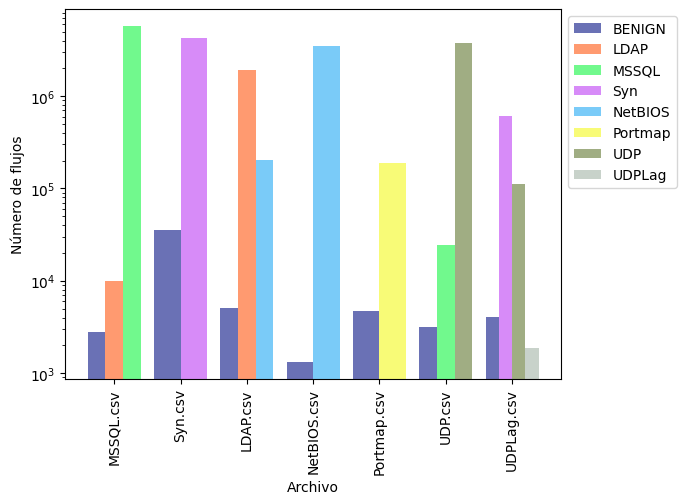
\includegraphics[width=\linewidth]{media/cicddos_2019_csv_03-11_file_results.png}
      \captionsetup{justification=centering}
      \caption{Número de flujos por archivo de las trazas de noviembre 3}\label{fig:cicddos_2019_csv_03-11_file_results}
    \endminipage\hfill
    \minipage{0.49\textwidth}
      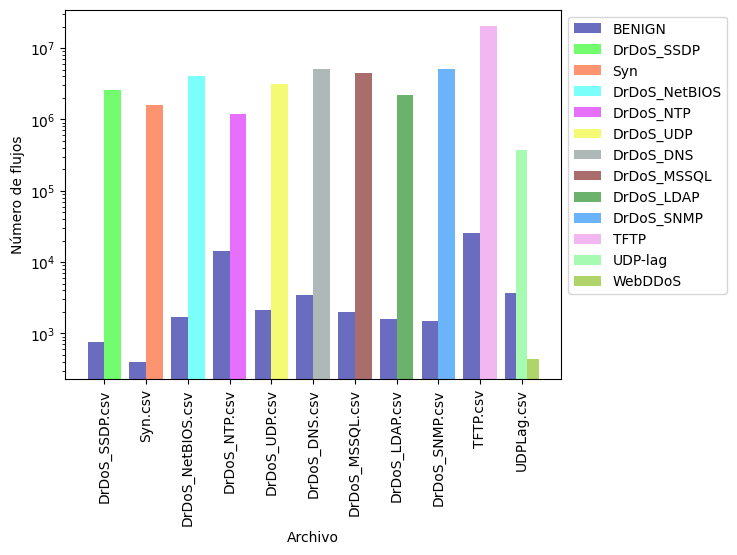
\includegraphics[width=\linewidth]{media/cicddos_2019_csv_01-12_file_results.png}
      \captionsetup{justification=centering}
      \caption{Número de flujos por archivo de las trazas de diciembre 1}\label{fig:cicddos_2019_csv_01-12_file_results}
    \endminipage\hfill
\end{figure}

\begin{figure}[!htb]
    \begin{center}
        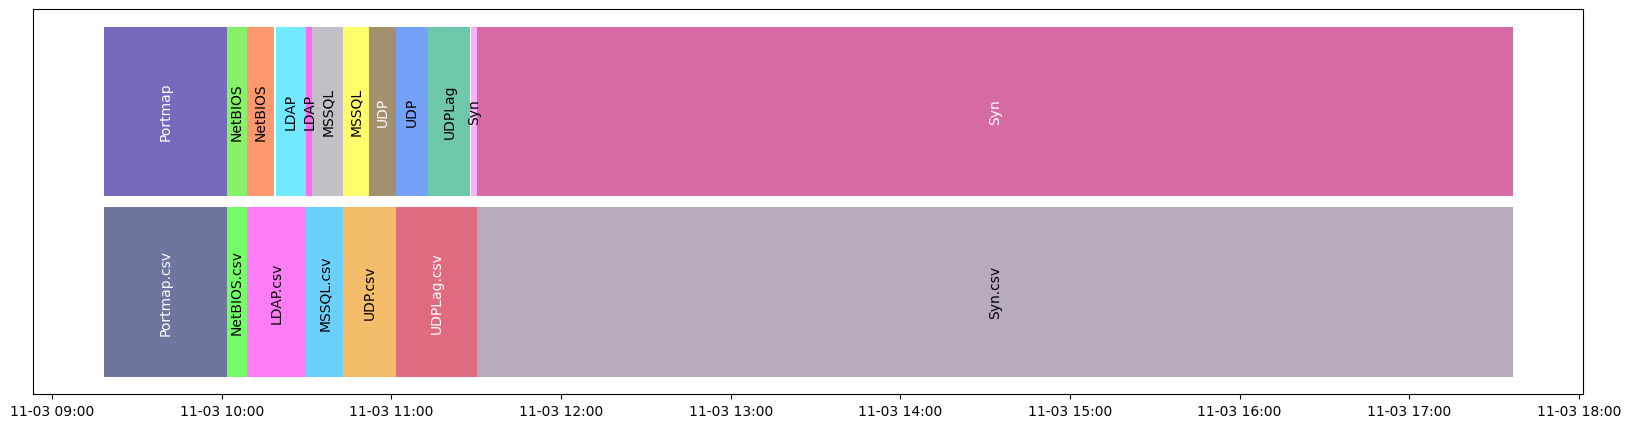
\includegraphics[width=1\linewidth]{media/cicddos_2019_csv_03-11_timeline.png}
    \end{center}
    \captionsetup{justification=centering}
    \caption{Línea temporal de las trazas de noviembre 3 con los archivos (debajo) y los rangos de ataques en estos (arriba)}\label{fig:cicddos_2019_csv_03-11_timeline}
\end{figure}
\begin{figure}[!htb]
    \begin{center}
        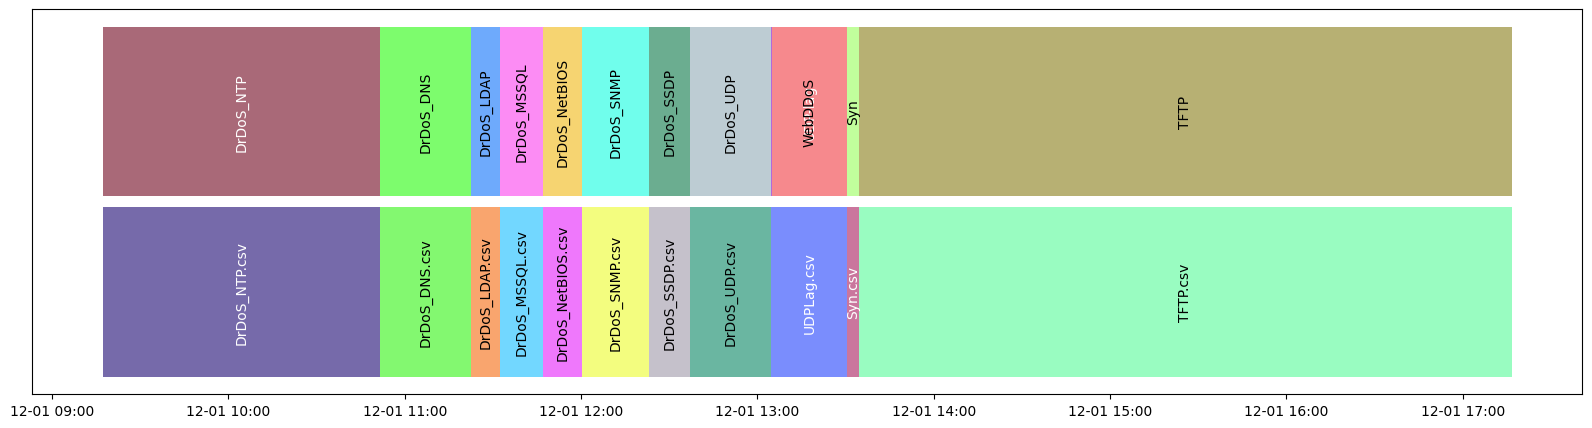
\includegraphics[width=1\linewidth]{media/cicddos_2019_csv_01-12_timeline.png}
    \end{center}
    \captionsetup{justification=centering}
    \caption{Línea temporal de las trazas de diciembre 1 con los archivos (debajo) y los rangos de ataques en estos (arriba)}\label{fig:cicddos_2019_csv_01-12_timeline}
\end{figure}

%\begin{figure}[!htb]
%    \minipage{1\textwidth}
%      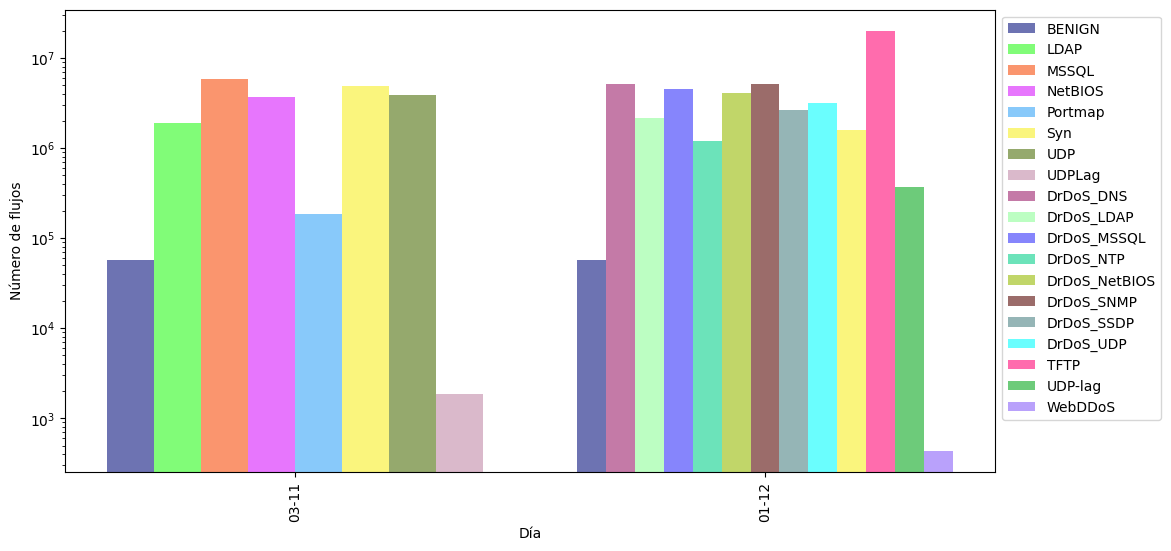
\includegraphics[width=\linewidth]{media/cicddos_2019_csv_day_results.png}
%      \captionsetup{justification=centering}
%      \caption{Número de flujos por archivo de las trazas de noviembre 3}\label{fig:cicddos_2019_csv_day_results}
%    \endminipage
%\end{figure}

\subsubsection{Contenidos pcaps}

El dataset CICDDos2019 ofrece un conjunto de trazas de red de los dos días en los que se generaron datos. Para el primer día (3 de noviembre), hay 145 archivos de unos 190.7 MiB cada uno y un último de 66.5 MiB. Para el segundo día (1 de diciembre), se ofrecen 818 archivos de 190.7 MiB cada uno y uno adicional de 3.7 MiB. En ambos casos, si intentamos abrir el último paquete con Wireshark o generamos cualquier análisis a través de tshark, se nos notifica que el paquete se encuentra 'cortado'. Esto es quizá causado porque, en el momento de generar las trazas, se cortó el proceso de captura precipitadamente. Los scripts utilizados para la extracción de datos es \texttt{extract\_info\_cicddos\_2019\_pcaps\_tshark.sh} y el utilizado para la representacion de estos es \texttt{evaluate\_info\_cicddos\_2019\_pcaps\_tshark.py} disponibles en TODO DEFINIR.

En los pcap, aparecen más direcciones IP en la red del testbed (192.\-168.\-50.\-0/24) de las mencionadas en la información ofrecida en la web del dataset. Concretamente, tenemos que en el primer día aparecen adicionalmente 192.\-168.\-50.\-4, 192.\-168.\-50.\-9 192.\-168.\-50.\-253 y 192.\-168.\-50.\-254. En el segundo día, tenemos que aparecen 192.\-168.\-50.\-253 y 192.\-168.\-50.\-254 además del posible router con IP 192.\-168.\-50.\-1. Adicionalmente, en ambos casos aparece la IP de broadcast (192.\-168.\-50.\-255). Respecto al número de direcciones IP únicas, podemos ver que en el primer día aparecen 1321 y en el segundo 640, teniendo en total 1723 únicas en el transcurso de los dos días. 

Se han generado histogramas con la distribución de la duración de los flujos, número de tramas y número de bytes para poder compararlos con los futuros resultados de la herramienta y comprobar que son consistentes. Como podemos ver en la Figura \ref{fig:cicddos_2019_pcap_duration_distribution}, hay muchos flujos los cuales su duración es relativamente corta y luego hay cierta variedad de flujos de mayor duración. Para el caso de las tramas, podemos observar en la Figura \ref{fig:cicddos_2019_pcap_frames_distribution} que en su mayoría se concentran entre 1 y 1000 tramas y a continuación se reduce drásticamente la cantidad, aunque hay un grupo de flujos los cuales se comprenden entre 10 000 y 100 000. En la Figura \ref{fig:cicddos_2019_pcap_bytes_distribution}, podemos ver que tenemos un caso similar, la mayoría se concentra en las partes bajas, después decrece y hay un grupo numeroso separado el cual realiza una gran transferencia de datos.

\begin{figure}[H]
    \begin{center}
        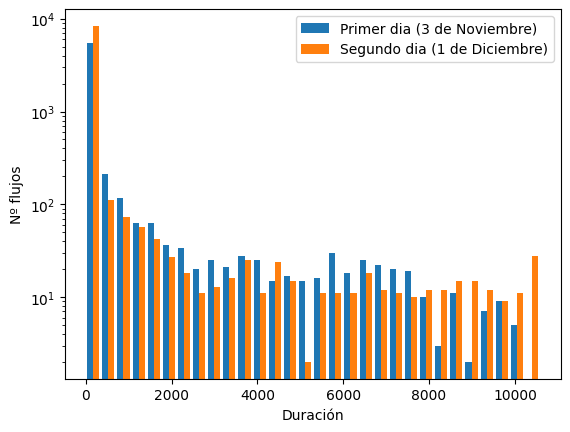
\includegraphics[width=0.49\linewidth]{media/cicddos_2019_pcap_duration_distribution.png}
    \end{center}
    \captionsetup{justification=centering}
    \caption{Distribución duraciones de flujos en CICDDos2019}\label{fig:cicddos_2019_pcap_duration_distribution}
\end{figure}

\begin{figure}[H]
    \minipage{0.49\textwidth}
      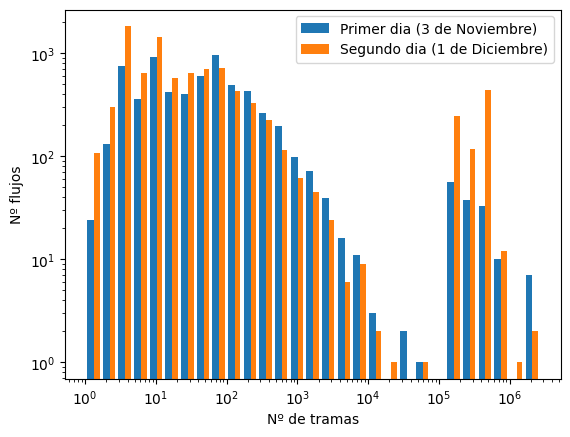
\includegraphics[width=\linewidth]{media/cicddos_2019_pcap_frames_distribution.png}
      \captionsetup{justification=centering}
      \caption{Distribución número de tramas en flujos en CICDDos2019}\label{fig:cicddos_2019_pcap_frames_distribution}
    \endminipage\hfill
    \minipage{0.49\textwidth}
      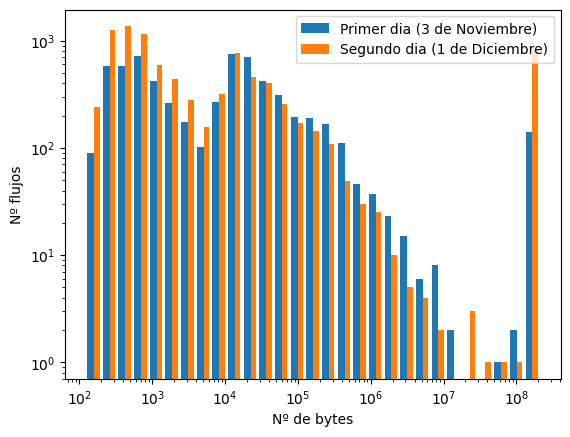
\includegraphics[width=\linewidth]{media/cicddos_2019_pcap_bytes_distribution.png}
      \captionsetup{justification=centering}
      \caption{Distribución número de bytes en flujos en CICDDos2019}\label{fig:cicddos_2019_pcap_bytes_distribution}
    \endminipage\hfill
\end{figure}

Si miramos la cantidad de información transmitida por las diferentes capas de red y de transporte en la tabla \ref{table:cicddos2019protocols}, podemos ver cómo la mayor parte del tráfico consiste en UDP, TCP y otro que tshark no ha podido identificar (data). De los 174.8 GiB transmitidos en total, menos de 10 MiB consisten en tráfico no IPv4. Adicionalmente, un 66.01\% de este tráfico es específicamente UDP, haciendo uso de posibles diversos protocolos en la siguiente capa. Es posible que la cantidad de protocolos sea engañosa, ya que es posible que este número haya sido exagerado a causa de ataques de escaneo en el dataset. Los otros dos puestos sobre la capa de red, consisten en 57.1 GiB (32.66\%) que tshark no pudo identificar y 2.2GiB (1.25\%) de tráfico TCP. 

%Generated with /workspaces/tfg/scripts/evaluate_info_cicddos_2019_pcaps_tshark.py
\begin{table}[H]
    \begin{center}
        \begin{tabular}{|c c c | c c c|} 
            \hline
            \textbf{L0} & \textbf{L1} & \textbf{L2} & \textbf{Tramas} & \textbf{Bytes} & \textbf{Nº subprotocolos}\\
            \hline\hline
eth &- &- & 3.12e+08 & 174.8GiB & 5 \\
eth &ip &- & 3.12e+08 & 174.8GiB & 7 \\
eth &ip &data & 4.44e+07 & 57.1GiB & 0 \\
eth &ip &udp & 2.42e+08 & 115.4GiB & 187 \\
eth &ip &icmp & 2.01e+05 & 29.9MiB & 64 \\
eth &ip &tcp & 2.56e+07 & 2.2GiB & 7 \\
eth &ip &ospf & 4.42e+04 & 4.0MiB & 0 \\
eth &ip &igmp & 1.00e+02 & 5.9KiB & 0 \\
eth &ip &rsvp & 2.00e+00 & 260.0B & 0 \\
eth &llc &- & 3.54e+04 & 3.0MiB & 3 \\
eth &llc &stp & 2.93e+04 & 1.8MiB & 0 \\
eth &llc &dtp & 3.90e+03 & 228.8KiB & 0 \\
eth &llc &cdp & 2.17e+03 & 977.2KiB & 0 \\
eth &ipv6 &- & 2.00e+04 & 2.9MiB & 2 \\
eth &ipv6 &udp & 1.54e+04 & 2.5MiB & 5 \\
eth &ipv6 &icmpv6 & 4.59e+03 & 418.5KiB & 0 \\
eth &arp &- & 9.14e+03 & 535.6KiB & 0 \\
eth &lldp &- & 1.22e+02 & 7.1KiB & 0 \\
            \hline
        \end{tabular}
    \end{center}
    \caption{Primeras tres capas de protocolos identificados en CICDDos2019}
    \label{table:cicddos2019protocols}
\end{table}


\subsection{BoT-IoT}

(por hacer)

\subsection{TON-IoT}

(por hacer)

\subsection{UNSW-NB15}

(por hacer)


\section{Formatos y protocolos de red}

En esta sección definiremos los diferentes protocolos y formatos de red que serán tenidos en cuenta. Concretamente, veremos el formato 'libpcap' en el que las trazas de red son guardadas, las capas de enlace de Ethernet y Linux Cooked Capture v1 (SLL), las capas de red IPv4 e IPv6 y las capas de transporte UDP y TCP.

\subsection{libpcap}

\subsubsection{Descripción}

El formato libpcap es un formato de captura de trazas de red utilizado en TcpDump, WinDump, Wireshark, entre otros \cite{pcapfileformatwireshark} \cite{pcapfileformatrfc}. La estructura general consiste en una cabecera de fichero y a continuación uno cero o más 'Packet Records' o registros de paquetes. Cada uno de estos contiene una cabecera con información de la captura y bytes provenientes del paquete capturado. Adicionalmente, el orden de los campos de los bits dentro de las cabeceras depende del formato nativo de la máquina donde se capturaron los paquetes. 

\subsubsection{Cabecera de fichero}

\begin{figure}[H]
    \begin{center}
        \begin{bytefield}{32}
            \bitheader{0-31} \\
            \bitbox{32}{Número mágico} \\
            \bitbox{16}{Versión mayor} 
            \bitbox{16}{Versión menor} \\
            \bitbox{32}{Reservado 1} \\
            \bitbox{32}{Reservado 2} \\
            \bitbox{32}{Longitud máxima capturada} \\
            \bitbox{3}{FCS} & \bitbox{1}{f}
            \bitbox{28}{Tipo capa de enlace} \\
            \bitheader{0-31} \\
        \end{bytefield}
    \end{center}
    \caption{Formato cabecera archivo libpcap}
    \label{fig:libpcap_file_header}
\end{figure}

El orden de los campos en la cabecera del fichero es como podemos ver en la Figura \ref{fig:libpcap_file_header}. El significado de los campos es el siguiente:

\begin{enumerate}
    \item \textbf{Número mágico}: Permite identificar el archivo como pcap, conocer la precisión de los campos de tiempo y saber el orden de bits de las cabeceras. El valor del campo en hexadecimal es \texttt{0xA1B2C3D4} si tenemos segundos y microsegundos. En caso de que sea \texttt{0xA1B23C4D}, tenemos precisión de nanosegundos en vez de microsegundos. Finalmente, si el primer byte del fichero tiene el valor \texttt{0xA1}, los campos tienen el orden 'big endian' (los bytes más significativos aparecen primero). En el caso opuesto, tienen el orden 'little endian' (los bytes menos significativos aparecen primero).
    \item \textbf{Versión mayor}: Valor no entero representando la versión semántica mayor \cite{preston2013semantic}. La última versión hasta la fecha es 2.
    \item \textbf{Versión menor}: Valor no entero, representando la versión semántica menor \cite{preston2013semantic}. La última versión hasta la fecha es la 4.
    \item \textbf{Reservado 1}: Valor no utilizado en la actualidad. En versiones antiguas se utilizaba para marcar la diferencia de huso horario.
    \item \textbf{Reservado 2}: Valor no utilizado en la actualidad. En versiones antiguas se utilizaba para indicar la precisión de las marcas de tiempo.
    \item \textbf{Longitud máxima capturada}: Número máximo de bytes de los paquetes originales que pueden ser incluidos en la traza de red. Si hay algún paquete que originalmente es más grande que este tamaño, se trunca a la longitud indicada.
    \item \textbf{FCS/f}: si el bit "f" está a 1, los siguientes 3 bits indican el número de bytes de detección de errores añadidos a continuación. 
    \item \textbf{Tipo capa de enlace}: Número identificando el tipo de la capa de enlace utilizado. Algunos ejemplos son 1 para IEEE 802.3 (Ethernet) o 113 para 'Linux Cooked Capture v1' \cite{linktypetcpdump}
\end{enumerate}

\subsubsection{Registro de paquete}

El orden de los campos en la cabecera del fichero es como podemos ver en la Figura \ref{fig:libpcap_file_packet_record}. La marca se encuentra representada como el número de segundos y micro/nanosegundos (dependiendo de la cabecera del fichero) transcurridos desde el 1 de enero de 1970 a las 00:00 UTC. Se incluye el tamaño del paquete original y el capturado, ya que no todos los paquetes de la captura tienen necesariamente el mismo tamaño que el original ni entre ellos.

\begin{figure}[h]
    \begin{center}
        \begin{bytefield}{32}
            \bitheader{0-31} \\
            \bitbox{32}{Marca de tiempo (parte de segundos)} \\
            \bitbox{32}{Marca de tiempo (parte de micro/nanosegundos)} \\ 
            \bitbox{32}{Tamaño del paquete capturado} \\
            \bitbox{32}{Tamaño del paquete original} \\
            \wordbox{3}{Datos del paquete} \\
        \end{bytefield}
    \end{center}
    \caption{Formato registro de paquete archivo libpcap}
    \label{fig:libpcap_file_packet_record}
\end{figure}

\subsection{Ethernet}

por hacer

\subsection{Linux Cooked Capture v1 (SLL)}

por hacer

\subsection{IP versión 4}

por hacer

\subsection{IP versión 6}

por hacer

\subsection{UDP}

por hacer

\subsection{TCP}

por hacer

\section{Software para el desarrollo}

En esta sección resumiremos los diferentes elementos software que serán utilizados para el desarrollo del trabajo. Concretamente, se indicarán los lenguajes de programación utilizados y los programas, además de la razón de su uso.

\subsection{Lenguajes de programación}

\subsubsection{Rust}

Rust es un lenguaje de programación compilado de propósito general y multiparadigma \cite{blandy2017programming} \cite{klabnik2018rust}. Este trata de garantizar que todas las referencias a memoria sean válidas e impedir condiciones de carrera sin tener necesidad de un 'recolector de basura' como Java o Python. Esto lo hace a través de, en el momento de compilación, comprobar que los usos de memoria sean correctos. 

Debido a que garantizar con exactitud si un programa hace uso de la memoria de forma correcta es un reto, el compilador toma una posición más conservadora. En caso de que el programador tenga más información y sepa que un uso de memoria que el compilador rechaza es correcto, existen métodos para hacer que el compilador lo acepte. Ejemplos son el uso de \texttt{unwrap()} para acceder a valores opcionales, el cual, si no contiene el valor esperado, interrumpe el programa en vez de corromper la memoria, o bloques \texttt{unsafe}, donde el programador ha de manualmente comprobar que no se está accediendo a memoria inválida.

Se ha escogido este lenguaje para el desarrollo de la herramienta debido a la capacidad de escribir código de bajo nivel, su alto rendimiento, su énfasis en el código correcto, la calidad de las herramientas asociadas y el gran número de librerías disponibles. 

\subsubsection{Bash}

\color{blue} %TODO remove this when revised

Bash, también conocido como GNU Bash, es un programa Shell y un lenguaje de comandos asociado que formaba originalmente parte del sistema operativo GNU \cite{gnubashweb} \cite{gnubashmanual}. Se puede ejecutar de forma interactiva, donde escribimos los comandos directamente en el terminal, o de manera no interactiva, donde le pasamos un archivo con la lista de comandos a ejecutar. Los comandos pueden ser palabras intrínsecas del lenguaje (\texttt{if}, \texttt{do}, entre otros) o programas para ser ejecutado. Adicionalmente, tiene soporte para bucles, guardar y expandir variables, funciones, listas, ente otros.

Se ha escogido Bash porque es la Shell utilizada por defecto en muchas distribuciones Linux. Con esta, automatizaremos tareas que requieran tratar archivos con herramientas existentes, como por ejemplo \texttt{tshark}.

\subsubsection{Python}

Python es un lenguaje de programación interpretado de propósito general y multiparadigma \cite{aboutpython} \cite{davepython}. Trata de focalizarse en la legibilidad del código y su facilidad de uso en la medida de lo posible. Esto lo hace a través de una librería estándar extensa, una gran cantidad de librerías creadas por la comunidad, tipos dinámicos y un 'recolector de basura' que permite a los desarrolladores no tener que gestionar memoria de forma manual.

Se ha escogido este lenguaje para las tareas que consistan en visualizar y tratar datos, además de las tareas de \gls{ml}, ya que es uno de los lenguajes frecuentemente utilizados para esto. Adicionalmente, las librerías disponibles y la documentación asociada facilitarán su uso.

\subsection{Programas}

\subsubsection{Git}

por hacer

\subsubsection{Docker}

por hacer

\subsubsection{Visual Studio Code}

por hacer


\newpage
\pagestyle{plain}

\chapter{MARCO PRÁCTICO}

\section{Entorno de desarrollo}

El entorno de desarrollo utilizado durante el transcurso del trabajo consiste en diversas partes. Como base tenemos el editor. En este, especificamos una configuración para desarrollar bajo un contenedor en el que se instalen automáticamente todas las dependencias necesarias.

Primero de todo, se ha hecho uso de Visual Studio Code como editor general para las diferentes partes del proyecto, como se ha indicado en el marco teórico. Adicionalmente, se ha utilizado una extensión llamada 'dev containers', la cual permite integrar el editor con un contenedor de docker \cite{devcontainers}. Esto nos permite adicionalmente conectarnos remotamente desde otros dispositivos y acceder al último estado del proyecto. Para configurarlo, se ha definido un archivo \texttt{devcontainer.json}, el cual nos permite indicar qué capas y configuración queremos que se genere en nuestro entorno. Esta configuración consiste en:

\begin{enumerate}
    \item Indicar la distribución Debian como imagen base
    \item La característica 'latex', la cual nos añade la extensión 'LaTeX Workshop' en el editor, además del compilador LaTeX para compilar la memoria. Adicionalmente, permite indicar la lista de librerías que se han de instalar.
    \item La característica 'Python', la cual nos instala tanto el interpretador Python como extensiones para tener autocompletado y capacidad de depurar el código.
    \color{blue} %TODO remove this when revised
    \item La característica 'apt-packages', la cual nos permite indicar paquetes a instalar de forma declarativa. Primero hemos indicado 'tshark', 'libpcap-dev', ya que son los que se han utilizado para realizar el análisis de las trazas de red y capturar paquetes, respectivamente. Después, se ha añadido 'openjdk-17-jre' para poder ejecutar PlantUML localmente.
    \color{black} %TODO remove this when revised
    \item La característica 'rust', la cual nos instala el compilador y el gestor de paquetes del lenguaje Rust además de extensiones para tener autocompletado, depuración, instalación de paquetes automática, entre otros.
    \color{blue} %TODO remove this when revised
    \item Un script para instalar dependencias adicionales. Estas consisten en tipos de letras utilizadas en la memoria, un entorno virtual de Python con los paquetes relevantes y la descarga de PlantUML desde GitHub para tener una versión más reciente que la ofrecida en la distribución base.
    \color{black} %TODO remove this when revised
    \item Dos directrices para incluir carpetas del host dentro del contenedor. Estos consisten en la carpeta de los datasets descargados (montada en /Datasets) y las credenciales SSH para firmar y subir cambios realizados en el sistema de control de versiones.
\end{enumerate}

Dentro del contenedor, los archivos se han estructurado de forma que tenemos una carpeta para el código fuente de la herramienta, una carpeta para la memoria y otra para todos los scripts de análisis y extracción de datos. Adicionalmente, hay carpetas y archivos de configuración para el editor, contenedor, dependencias Python y control de versiones.

Finalmente, todos los archivos relevantes están bajo el control de versiones git. Para prevenir la posibilidad de perder los datos si el dispositivo en el que se encuentran guardados dejará de funcionar, se ha configurado un repositorio en GitHub para mantener una copia. Este se encuentra en \url{https://github.com/RabadanDotDev/tfg} y será hecho público una vez se haya realizado el depósito del trabajo.


\section{Desarollo packet pincer}

En esta sección veremos el funcionamiento de cada parte de la herramienta, la cual se ha llamado 'packet pincer' por el momento. Veremos qué y cuáles argumentos de consola acepta, como realiza la lectura de paquetes tanto en tiempo real como por trazas. A continuación se explicarán los diferentes pasos que se llevan a cabo en el momento de analizar un paquete y como se realiza la generación de estadísticas. Finalmente, veremos como se realiza el etiquetado automático de los flujos y se emiten los resultados.

Un esquema del flujo principal de la aplicación se puede observar en la Figura \ref{fig:packetpincerexecution}. Como podemos ver, se van extrayendo paquetes mientras se encuentren disponibles. Cuando se obtiene uno, en caso de ser un paquete \acrshort{ipv4} fragmentado, se intenta reconstruir o se guarda en caso de no poder. A continuación, se comprueba si la herramienta soporta analizar el paquete indicado y, en caso afirmativo, acumula la información en el flujo de transporte respectivo. Finalmente, se 'cierran' los flujos antiguos, es decir, se emite la información relevante y a continuación se descarta el resto de información acumulada.

\begin{figure}[H]
  \begin{center}
    \centering
    \resizebox{!}{\dimexpr\textheight-2\baselineskip\relax}{%
      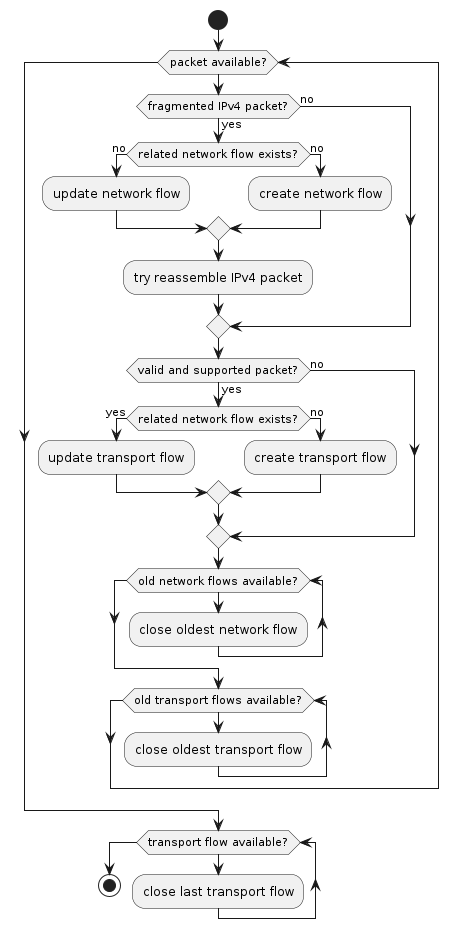
\includegraphics{plant_uml_diagrams/general_tool_loop.png}
    }
  \end{center}
  \caption{Flujo de la aplicación durante su ejecución}\label{fig:packetpincerexecution}
\end{figure}

\subsection{Argumentos y señales}

El programa está pensado para ser ejecutado desde el terminal. Debido a esto, hemos de definir que argumentos se pueden pasar al programa y hacer que este reaccione a señales del sistema operativo. Los argumentos suelen ser pasados desde el mismo comando utilizado para ejecutar el programa, siendo un ejemplo '\texttt{packet\_pincer \underline{help}}'. Las señales a su vez se pueden enviar utilizando una combinación de teclado como \texttt{CTRL+C} o utilizando otro programa.

Para hacer la gestión de los argumentos enviados por el terminal, se ha hecho uso de la librería (o 'crate', en la nomenclatura utilizada en Rust) clap \cite{Knapp_clap_2024}. Concretamente, se ha hecho uso de la funcionalidad 'derive', la cual permite expresar los argumentos a pasar como un tipo del lenguaje de forma declarativa. Adicionalmente, la librería añade diversas funcionalidades que mejoran la experiencia de usuario. A partir de nuestras definiciones, se muestran unas indicaciones de uso si se ejecuta \texttt{packet\_pincer --help} o si se pasan argumentos inválidos. Los argumentos definidos para el programa consisten en:

\begin{enumerate}
  \item Opcionalmente, indicar si escribir los resultados generados en archivos o en la salida estándar. Si no se especifica, no se emite nada.
  \item Opcionalmente, indicar un archivo con etiquetas para los flujos. En caso de que se especifique este archivo y no haya etiqueta correspondiente para un flujo determinado, se asignará 'benign'
  \item Indicación del origen de los paquetes a analizar. Este puede ser 'offline' (a partir de una traza de red o un directorio de estas) u 'online' (a partir de una interficie de red).
\end{enumerate}

Respecto a las señales, se hace uso de la librería ctrlc \cite{controlc}. Esta permite detectar señales de interrupción enviadas por el usuario para interrumpir la ejecución de la aplicación. Si el programa no respondiese a estas señales, el sistema operativo terminaría el proceso directamente. Esto podría provocar la escritura parcial de los archivos, potencialmente corrompiéndolos. En caso de que se genere una señal de interrupción del programa, lo tratamos como que no hay más paquetes disponibles.

El código que se encarga de tratar estos puntos, se puede encontrar en \texttt{main.rs} en el anexo 2 o en el repositorio de GitHub.

\subsection{Lectura de paquetes}

\subsubsection{Librerias}

Para realizar la lectura de paquetes, tanto en tiempo real como a partir de archivos, se ha escogido hacer uso de la librería de rust 'pcap' \cite{rustpcap}, la cual a su vez hace uso internamente de otra llamada 'libpcap' la cual es desarrollada por el grupo tcpdump \cite{libpcap}. Dependiendo de si queremos leer paquetes desde un archivo o desde una interfaz de red, tendremos que utilizar una función de la API pública u otra para generar una instancia 'Capture'. 

\subsubsection{Detalles de implementación comunes}

A pesar de que la librería ofrece casi todas las funcionalidades que se requieren, no ofrece soporte para leer desde una lista de archivos, sino que hemos de leer de cada uno individualmente. Debido a esto, se ha creado la envoltura 'PacketCapture' disponible en \texttt{packet\_capture.rs} en el anexo 2 o en el repositorio de GitHub. En esta, se permite crear una instancia a partir de una ruta, que puede ser un archivo, un directorio o una interfaz de red. Adicionalmente, permite al usuario del módulo hacer una petición para procesar el siguiente paquete. Esto se hace a través de pasar una clausura que acepta un 'PacketOrigin' (ruta del archivo o nombre, interfaz), un 'LinkType' (el tipo de la capa de enlace \cite{linktypetcpdump}) y una referencia al paquete a tratar. La función de procesamiento extrae el siguiente paquete y llama a la clausura, devolviendo un valor afirmativo si se ha podido extraer un paquete o un valor negativo en caso contrario.

Se hace uso de una clausura en vez de devolver una referencia al paquete debido a que el compilador no lo permitía. Después de investigar, esto era causado por el hecho que la librería pcap, dentro de la instancia 'Capture', tenía una referencia a un trozo de memoria. Al seguir manteniendo una referencia a la captura después de ejecutar la función, esto causaba que el compilador no pudiese garantizar que esta referencia fuese válida. En cambio, al pasar una clausura se puede asegurar que se haga un uso correcto de la memoria al poder indicarlo en el prototipo de la función proporcionada por el usuario del módulo.

\subsubsection{Lectura de paquetes en tiempo real}

Para el caso de la lectura de paquetes en tiempo real, podemos hacer uso relativamente directo de la librería. En el momento de crear 'PacketCapture' creamos la instancia 'Capture' basada en una interficie de red. Cuando queremos procesar el siguiente paquete, pasamos la petición directamente a 'Capture' y a continuación ejecutamos la clausura. Si no hay errores, devolvemos un valor verdadero, indicando que hay potencialmente más paquetes válidos. En caso contrario, indicamos un valor negativo, indicando que probablemente no se puedan capturar más paquetes.

\subsubsection{Lectura de trazas de paquetes}

El caso de la lectura de trazas es más complicado. Debido a que se quiere admitir el poder leer de uno o varios archivos, es necesario hacer una mayor gestión adicional a la que nos proporciona la librería. Para esto, se han definido tres estructuras internas:
\begin{enumerate}
  \item \textbf{OwnedPacket}: Un paquete el cual 'posee' la memoria a la que hace referencia. A diferencia del que nos proporciona la librería pcap, no hace referencia a una sección de memoria que puede formar o no parte de otra mayor, permitiéndonos garantizar que las referencias a memoria son válidas.
  \item \textbf{FileCapture}: Una envoltura de una 'Capture' de la librería pcap con su ruta de origen y el siguiente paquete que se debe tratar extraído. Esto se hace para poder ordenar las diferentes 'FileCapture' según el tiempo de captura del paquete.
  \item \textbf{FileCaptureCollection}: Un conjunto de 'FileCapture'. Está estructurado en dos campos: un 'HashMap' de la librería estándar y en una cola de prioridad \cite{priority-queue}. El primero es utilizado para poder acceder en tiempo constante a cualquier 'FileCapture' a partir de su ruta y el segundo para tener una lista ordenada de más a menos antiguo del siguiente paquete a analizar. Esto es necesario debido a que algunos conjuntos de datos contienen archivos que se solapan en el tiempo.
\end{enumerate}

Para generar la instancia a partir de la ruta, navegamos por todos los archivos y directorios de esta haciendo uso de walkdir \cite{walkdir}. Por cada archivo, intentamos abrirlo como captura pcap y, en caso de no ser posible, lo saltamos. Una vez abierto, extraemos el primer paquete de la captura y creamos un 'FileCapture' con las tres partes necesarias. Finalmente, creamos el 'HashMap' con todas las capturas abiertas y la cola de prioridad para poder acceder a las capturas de forma ordenada.

Para procesar el siguiente paquete, primero se obtiene la ruta de la captura con el siguiente paquete más antiguo. A continuación, se encuentra la instancia 'FileCapture' y llamamos a la clausura con esta. Una vez hecho esto, se trata de extraer el siguiente paquete de la traza de red. En caso de error, eliminamos la captura tanto de la cola como del 'HashMap'. En caso contrario, actualizamos el valor del siguiente paquete en 'FileCapture' y su posición en la cola.

\subsubsection{Obtención de paquetes} \label{obtencionpaquetes}

El uso de la envoltura \texttt{PacketCapture} se realiza desde \texttt{main.rs} disponible en el anexo 2 y en el repositorio. Una vez creada a partir de los argumentos proporcionados, se define una clausura para proporcionarlas a la función de procesamiento. A continuación se hace uso de un bucle infinito que llama a la función \texttt{try\_process\_next} en \texttt{PacketCapture}, pasando la clausura como argumento. Esto se realiza hasta que la función devuelve un valor falso o se reciba una señal de terminación. Dentro de la clausura, se acumula información en una instancia de \texttt{FlowGroup} (donde se decodifica el paquete y se acumula la información relevante del paquete), se actualizan las estadísticas de ejecución y se emiten estadísticas de flujos finalizados.

\subsection{Decodificación de paquetes y extensión de librería de código abierto} \label{packetdecode}

\subsubsection{Análisis librería}

Los datos ofrecidos por la librería \texttt{pcap} consisten en información de cuándo se capturó el paquete, cuál era la capa de enlace y los datos en crudo capturados. Es decir, nos interpreta exclusivamente la parte del formato 'libpcap' vista en \ref{libpcapformat}. Para interpretar el resto de capas indicadas en \ref{netformats}, haremos uso de la librería \texttt{etherparse} \cite{etherparse}.

Después de un primer análisis, se observó que la librería soportaba interpretar tramas de Ethernet \ref{etherformat}, paquetes \acrshort{ip} \ref{ipformat}, datagramas \acrshort{udp} \ref{udpformat} y segmentos \acrshort{tcp} \ref{tcpformat}. Sin embargo, no ofrecía soporte para \acrshort{sll} \ref{sllformat}, el cual necesitábamos para el dataset TON-IoT. Debido a que la librería tenía soporte para la mayoría de puntos necesarios, además de ofrecer una interfaz sencilla, se decidió hacer una extensión de esta para añadirle soporte de \acrshort{sll}. 

\subsubsection{Extensión librería}

Para realizar esto, primero se creó un 'issue' en el repositorio original el 24 de abril de 2024 para indicar al desarrollador de la librería sobre la intención de hacer esta adición \cite{slladdsllissue}. No se recibió respuesta, pero se inició el trabajo para añadir el soporte. Durante los siguientes 5 días, se añadieron 4145 líneas de código y se eliminaron 141. En estas, se incluye el formato \acrshort{sll}, el proceso para extraer los valores relevantes desde datos en crudo desde el formato \acrshort{sll}, tests y toda la documentación asociada. Se trató de mantener el estilo de la librería para asegurar que el desarrollador original aceptara los cambios. Una vez finalizado, el 29 de abril se creó un 'pull request' para juntar los cambios \cite{slladdsllpr}. En esta instancia, el desarrollador contestó agradeciendo el trabajo realizado. Después de que lo revisara y arreglase algunos detalles de integración, el 2 de mayo se juntaron los cambios a la rama principal.

\subsubsection{Uso de la libreria}

El primer uso durante el flujo del programa es en la función \texttt{try\_parse\_packet} disponible en \texttt{packet\_parse.rs} en el anexo 2 o en el repositorio. La función se llama después de realizar la extracción de un paquete desde \texttt{PacketCapture} o después de hacer una reconstrucción como veremos en \ref{ipv4defrag}. Dentro de la función, a partir del tipo de capa de enlace indicado por \texttt{pcap} y la librería etherparse, obtenemos una instancia de \texttt{SlicedPacket} de la cual podemos obtener los campos de diferentes capas del paquete original. En caso de datos Ethernet, utilizamos la función \texttt{etherparse::SlicedPacket::from\_ethernet} y en caso de tener datos en \acrshort{sll}, hacemos uso de {etherparse::SlicedPacket::from\_linux\_sll} añadida durante el desarrollo del proyecto.

\subsection{Obtención de identificadores} \label{idextraction}

Como se indicó en los puntos anteriores, después de obtener un paquete tratamos de primero decodificarlo y acumular la información relevante. Para poder hacer una diferenciación de las diferentes comunicaciones, extraemos un 'identificador del flujo' para poder clasificarla.

En la herramienta, consideramos dos casos de identificadores. Primero, un 'identificador de red', el cual usamos en los paquetes que portan un paquete \acrshort{ipv4} fragmentado. Para la identificación, hacemos uso de las direcciones de origen y destino, además del campo 'identifier' disponible en la cabecera \acrshort{ipv4}. A continuación, un 'identificador de transporte', el cual es utilizado cuando tratamos con un paquete \acrshort{ip} versión 4 o 6 y porta un datagrama \acrshort{udp} o un segmento \acrshort{tcp}. En este caso, utilizamos cinco valores para la identificación. Estos consisten en las direcciones de origen y destino, los puertos de origen y destino y finalmente el identificador del protocolo de la capa de transporte. En caso de no darse uno de los casos considerados, se emite un error indicando la razón (sin capa de red, de transporte o protocolo no soportado).

Una vez obtenido el identificador del paquete, si tenemos un identificador de red, se realiza paso de desfragmentación (\ref{ipv4defrag}). En caso de que tengamos un identificador de transporte o hayamos podido reconstruir el paquete, procederemos a acumular la información en el flujo de transporte respectivo (\ref{flowseparation}).

\subsection{Desfragmentación IPv4} \label{ipv4defrag}

Los datasets utilizados contienen tramos donde hay una gran cantidad de paquetes \acrshort{ipv4} fragmentados. Es posible que estén relacionados con ataques y que, si ofrecemos soporte para la desfragmentación en la herramienta, las estadísticas generadas puedan ser más útiles para la detección de ataques. Para realizar esto, se ha definido una estructura llamada \texttt{NetworkFragmentFlow}, la cual acumula fragmentos \acrshort{ipv4} con información adicional para su posterior reensamblado. Adicionalmente, en el momento de hacer un reensamblado, aparte del paquete reconstruido, se emitirá una estructura \texttt{FragmentReasemblyInformation} con la información adicional acumulada. Los diferentes flujos activos serán agrupados en la instancia \texttt{FlowGrup}, donde adicionalmente tendremos flujos de transporte como veremos en \ref{flowseparation}.

Para hacer la gestión de la desfragmentación de paquetes \acrshort{ipv4}, contamos con dos atributos en \texttt{FlowGroup}. Primero tenemos un \texttt{HashMap} para poder acceder en tiempo constante a cualquier flujo de red activo a partir de su identificador. A continuación, contamos con una cola para tener la lista de identificadores ordenada por el primer paquete encontrado para poder ser capaces de descartar flujos con este criterio. Con esto, por cada paquete que obtengamos, encontramos el flujo de red activo con el mismo identificador y lo actualizamos con el paquete obtenido. En caso de no encontrarlo, lo creamos. Adicionalmente, después de realizar la inclusión, comprobamos si podemos reconstruir el paquete. En caso positivo, lo hacemos y eliminamos el flujo tanto de la lista de flujos activos como de la cola.

Para evitar que la memoria crezca sin límites en caso de que no se puedan reconstruir los paquetes, \texttt{FlowGroup} contiene dos funciones para extraer el flujo 'más antiguo', siendo este el flujo el cual su primer paquete es el que tiene la marca de tiempo menor. La primera es incondicional, mientras que la segunda permite indicar una antigüedad mínima respecto del último paquete procesado. Mientras que procesa paquete a paquete, se ha impuesto un límite de un minuto de antigüedad máxima. En el momento de finalización del análisis, los paquetes restantes son descartados. 

Respecto \texttt{NetworkFragmentFlow}, internamente contiene diversos valores. Entre estos, se encuentran el tiempo del primer paquete procesado, el tiempo del último procesado, el tamaño esperado del paquete completo, los bytes del campo de datos de los fragmentos y el recuento total de los fragmentos con sus bytes recibidos. Con esta información, en el momento de hacer la reconstrucción, podemos comprobar si no nos quedan huecos entre los bytes. En caso negativo, utilizamos la última cabecera del paquete recibido y le substituimos el campo de datos por los datos reconstruidos. Adicionalmente, generamos una instancia de \texttt{FragmentReasemblyInformation} con la información adicional acumulada (tiempos, cantidades de paquetes y bytes recibidos en total) para poder tener estadísticas con mayor consistencia.

\subsection{Separación de flujos de transporte} \label{flowseparation}

Para la gestión de los flujos de transporte hacemos algo similar que con los flujos de red de paquetes fragmentados. Para correlacionar paquetes con flujos de comunicación, aparte de extraer los identificados en \ref{idextraction}, se ha de tener en cuenta que las direcciones y puertos origen/destino están invertidos en los mensajes de respuesta.

En el transcurso normal del protocolo \acrshort{tcp} existe una finalización de la transmisión explícita. Sin embargo, se ha de tener en cuenta la posibilidad de que la conexión se interrumpa sin esta. Adicionalmente, \acrshort{udp} no tiene ningún tipo de forma de indicar que una comunicación ha terminado. Por tanto, la gestión de considerar que un flujo ha terminado se ha basado en todos los casos en 'timeouts', es decir, se hace de una manera similar al 'descarte' que se realiza para los paquetes fragmentados. A pesar de hacerlo de forma similar, utilizaremos funciones separadas para poder tratar los dos niveles de forma distinta.

Para almacenar la información, también se hace uso de \texttt{FlowGroup}. En este, tenemos un \texttt{HashMap} para tener acceso en tiempo constante a los flujos y una cola de prioridad para mantener un orden temporal. En este caso, el criterio que se sigue consiste en tener los flujos que han tenido una recepción de un paquete más nuevo más atrás de la cola. Es decir, si en el flujo $A$ el último paquete ha sido en $t=10$ y en el flujo $B$ ha sido en $t=5$, el flujo $B$ se encontraría antes del flujo $A$. Cada vez que actualizamos la información de un flujo a partir de un paquete, actualizamos la posición de este para que esté al final de la cola.

\subsection{Generación de estadísticas} \label{statsgen}

Cada vez que, a partir de un paquete con un protocolo soportado, se crea o se identifica el flujo de transporte respectivo, se han de acumular una serie de datos para poder generar unas estadísticas del flujo. Cuando el flujo se considera finalizado o se 'cierra' y se emiten las estadísticas de este, se utiliza esta información acumulada para generarlas. Después, estos valores son emitidos como se indica en \ref{flowwrite}.

La información que se acumula durante el transcurso de la ejecución es diversa. Las estadísticas escogidas para generar han sido basadas en las utilizadas en CICFlowMeter como vimos en \ref{cicflowfeatures}. En conjunto, mantenemos:

\begin{itemize}
  \item La marca de tiempo del primer y último paquete
  \item Una lista de protocolos detectados. En el momento, lo hemos mantenido en sí, se ha detectado el protocolo \acrshort{tcp} y/o el protocolo \acrshort{udp}.
  \item El recuento de paquetes desde el que ha iniciado la emisión (forward) o hacia este (backward).
  \item Un \texttt{RunningStat} del número de bytes enviados en cada dirección (forward/backward) y en ambas (bidirectional).
  \item Un \texttt{RunningStat} del periodo de llegada entre paquetes en cada dirección (forward/backward) y en ambas (bidirectional). Adicionalmente, se mantiene una marca de tiempo del último paquete en cada dirección para facilitar el cálculo.
  \item El número de flags \acrshort{tcp} vistas en las dos direcciones. Adicionalmente, mantenemos un recuento separado de los flags PSH y URG de cada dirección.
  \item Un \texttt{RunningStat} para información específica sobre las longitudes en bytes de la cabecera de la capa de transporte y las longitudes de los campos de datos.
  \item El número de paquetes enviados desde el iniciador de la conexión con un campo de datos en la capa de transporte no vacía.
  \item El tamaño de la ventana inicial \acrshort{tcp} en cada dirección, si está disponible.
  \item Dos \texttt{RunningStat} para tener un recuento de los tiempos que el flujo ha estado activo (menos de un segundo de separación entre paquetes) e inactivo pero sin ser cerrado. Adicionalmente, hay un recuento de cuantos grupos activos ha habido.
\end{itemize}

Los \texttt{RunningStat} mencionados son utilizados para mantener, como su nombre indica, información estadística calculada de forma iterativa. Concretamente, mantenemos en cada uno el número de valores, la suma, el valor mínimo, el valor máximo, la media y la 'diferencia al cuadrado'. Esta ultima, la mantenemos como valor parcial para obtener la variancia y la distribución estándar, como se indica en la página 232 de 'The art of computer programming' \cite{10.5555/270146}. Específicamente, primero se define la recurrencia \ref{eq:meanrec} para calcular la media de forma iterativa. A continuación, se utiliza esta para obtener la recurrencia de la 'diferencia al cuadrado' mostrada en \ref{eq:sqrrec}, de la cual podemos obtener la varianza como se indica en \ref{eq:variancereq}. A partir de esta, podemos obtener la desviación estándar (\sigma).

\begin{equation} \label{eq:meanrec}
  \biggl\{
      \begin{array}{l}
        M_{0} = 0\\
        M_{k} = M_{k-1} + {{ x_{k} - M_{k-1} } \over {k}}  \\
      \end{array} 
\end{equation}

\begin{equation} \label{eq:sqrrec}
  \biggl\{
      \begin{array}{l}
        S_{0} = 0 \\
        S_{k} = S_{k-1} + ( x_{k} - M_{k-1} ) * ( x_{k} - M_{k} )
      \end{array}      
\end{equation}

\begin{equation} \label{eq:variancereq}
  \biggl\{
    \sigma^2_{k} = {S_{k} \over {(k - 1)}}
\end{equation}

Con esto, en el momento de cerrar el flujo y emitir las estadísticas, se generan los siguientes valores:

\begin{enumerate}
  \item \texttt{duration\_seconds}: duración en segundos del flujo.
  \item \texttt{has\_tcp}: 1 si se utiliza \acrshort{tcp} en el flujo, 0 en caso contrario.
  \item \texttt{has\_udp}: 1 si se utiliza \acrshort{udp} en el flujo, 0 en caso contrario.
  %%
  \item \texttt{bidirectional\_packet\_count}: el número total de paquetes enviados.
  \item \texttt{forward\_packet\_count}: el número total de paquetes enviados desde el iniciador de la transmisión.
  \item \texttt{backward\_packet\_count}: el número total de paquetes enviados hacia el iniciador de la transmisión.
  \item \texttt{bidirectional\_packet\_second}: la cadencia media de paquetes por segundo en ambas direcciones.
  \item \texttt{forward\_packet\_second}: la cadencia media de paquetes por segundo desde el iniciador de la transmisión.
  \item \texttt{backward\_packet\_second}: la cadencia media de paquetes por segundo hacia el iniciador de la transmisión.
  %%
  \item \texttt{bidirectional\_packet\_bytes\_sum}: suma total de bytes capturados de los paquetes capturados en ambas direcciones.
  \item \texttt{bidirectional\_packet\_bytes\_max}: tamaño del paquete más grande capturado en ambas direcciones.
  \item \texttt{bidirectional\_packet\_bytes\_min}: tamaño del paquete más pequeño capturado en ambas direcciones.
  \item \texttt{bidirectional\_packet\_bytes\_mean}: tamaño medio de los paquetes capturados en ambas direcciones.
  \item \texttt{bidirectional\_packet\_bytes\_std}: desviación estándar de los paquetes capturados en ambas direcciones.
  \item \texttt{forward\_packet\_bytes\_sum}: suma total de bytes capturados originados por el iniciador de la transmisión.
  \item \texttt{forward\_packet\_bytes\_max}: tamaño del paquete más grande capturado originado por el iniciador de la transmisión.
  \item \texttt{forward\_packet\_bytes\_min}: tamaño del paquete más pequeño capturado originado por el iniciador de la transmisión.
  \item \texttt{forward\_packet\_bytes\_mean}: tamaño medio de los paquetes capturados originados por el iniciador de la transmisión.
  \item \texttt{forward\_packet\_bytes\_std}: desviación estándar de los paquetes capturados originados por el iniciador de la transmisión.
  \item \texttt{backward\_packet\_bytes\_sum}: suma total de bytes capturados originados por el receptor inicial de la transmisión.
  \item \texttt{backward\_packet\_bytes\_max}: tamaño del paquete más grande capturado originado por el receptor inicial de la transmisión.
  \item \texttt{backward\_packet\_bytes\_min}: tamaño del paquete más pequeño capturado originado por el receptor inicial de la transmisión.
  \item \texttt{backward\_packet\_bytes\_mean}: tamaño medio de los paquetes capturados originados por el receptor inicial de la transmisión. 
  \item \texttt{backward\_packet\_bytes\_std}: desviación estándar de los paquetes capturados originados por el receptor inicial de la transmisión.
  \item \texttt{bidirectional\_bytes\_s}: cadencia media de datos en bytes por segundo en ambas direcciones.
  \item \texttt{forward\_bytes\_s}: cadencia media de datos en bytes por segundo desde el iniciador de la transmisión.
  \item \texttt{backward\_bytes\_s}: cadencia media de datos en bytes por segundo hacia el iniciador de la transmisión.
  \item \texttt{down\_up\_bytes\_ratio}: balance entre los bytes capturados entre las dos direcciones.
  %%
  \item \texttt{bidirectional\_inter\_arrival\_time\_max}: tiempo de llegada entre paquetes máximo en ambas direcciones.
  \item \texttt{bidirectional\_inter\_arrival\_time\_min}: tiempo de llegada entre paquetes mínimo en ambas direcciones.
  \item \texttt{bidirectional\_inter\_arrival\_time\_mean}: tiempo de llegada media de los paquetes en ambas direcciones.
  \item \texttt{bidirectional\_inter\_arrival\_time\_std}: desviación estándar del tiempo de llegada de los paquetes en ambas direcciones.
  \item \texttt{forward\_inter\_arrival\_time\_max}: tiempo de llegada entre paquetes máximo del iniciador de la transmisión.
  \item \texttt{forward\_inter\_arrival\_time\_min}: tiempo de llegada entre paquetes mínimo del iniciador de la transmisión.
  \item \texttt{forward\_inter\_arrival\_time\_mean}: tiempo de llegada media de los paquetes del iniciador de la transmisión.
  \item \texttt{forward\_inter\_arrival\_time\_std}: desviación estándar del tiempo de llegada de los paquetes del iniciador de la transmisión.
  \item \texttt{backward\_inter\_arrival\_time\_max}: tiempo de llegada entre paquetes máximo hacia el iniciador de la transmisión.
  \item \texttt{backward\_inter\_arrival\_time\_min}: tiempo de llegada entre paquetes mínimo hacia el iniciador de la transmisión.
  \item \texttt{backward\_inter\_arrival\_time\_mean}: tiempo de llegada media de los paquetes hacia el iniciador de la transmisión.
  \item \texttt{backward\_inter\_arrival\_time\_std}: desviación estándar del tiempo de llegada de los paquetes hacia el iniciador de la transmisión.
  %%
  \item \texttt{bidirectional\_tcp\_cwr\_flags\_count}: número de paquetes en ambas direcciones con el campo 'cwr' de la cabecera \acrshort{tcp} activo.
  \item \texttt{bidirectional\_tcp\_ece\_flags\_count}: número de paquetes en ambas direcciones con el campo 'ece' de la cabecera \acrshort{tcp} activo.
  \item \texttt{bidirectional\_tcp\_urg\_flags\_count}: número de paquetes en ambas direcciones con el campo 'urg' de la cabecera \acrshort{tcp} activo.
  \item \texttt{bidirectional\_tcp\_ack\_flags\_count}: número de paquetes en ambas direcciones con el campo 'ack' de la cabecera \acrshort{tcp} activo.
  \item \texttt{bidirectional\_tcp\_psh\_flags\_count}: número de paquetes en ambas direcciones con el campo 'psh' de la cabecera \acrshort{tcp} activo.
  \item \texttt{bidirectional\_tcp\_rst\_flags\_count}: número de paquetes en ambas direcciones con el campo 'rst' de la cabecera \acrshort{tcp} activo.
  \item \texttt{bidirectional\_tcp\_syn\_flags\_count}: número de paquetes en ambas direcciones con el campo 'syn' de la cabecera \acrshort{tcp} activo.
  \item \texttt{bidirectional\_tcp\_fin\_flags\_count}: número de paquetes en ambas direcciones con el campo 'fin' de la cabecera \acrshort{tcp} activo.
  \item \texttt{forward\_tcp\_psh\_flags\_count}: número de paquetes desde el iniciador de la transmisión con el campo 'psh' de la cabecera \acrshort{tcp} activo.
  \item \texttt{forward\_tcp\_urg\_flags\_count}: número de paquetes desde el iniciador de la transmisión con el campo 'urg' de la cabecera \acrshort{tcp} activo.
  \item \texttt{backward\_tcp\_psh\_flags\_count}: número de paquetes hacia el iniciador de la transmisión con el campo 'psh' de la cabecera \acrshort{tcp} activo.
  \item \texttt{backward\_tcp\_urg\_flags\_count}: número de paquetes hacia el iniciador de la transmisión con el campo 'urg' de la cabecera \acrshort{tcp} activo.
  %%
  \item \texttt{forward\_transport\_header\_bytes\_sum}: la suma total del número de bytes en las cabeceras de transporte de los paquetes del iniciador de la transmisión.
  \item \texttt{forward\_transport\_payload\_bytes\_mean}: la media del número de bytes de datos de la capa de transporte de los paquetes del iniciador de la transmisión.
  \item \texttt{forward\_transport\_payload\_bytes\_min}: el mínimo del número de bytes de datos de la capa de transporte de los paquetes del iniciador de la transmisión.
  \item \texttt{forward\_transport\_packets\_with\_payload\_count}: el número de paquetes del iniciador de la conexión con el campo de datos de la capa de transporte no vacío.
  \item \texttt{forward\_tcp\_initial\_window\_bytes}: la ventana \acrshort{tcp} inicial, o número de bytes aceptados, por parte del iniciador de la transmisión, si aplica.
  \item \texttt{backward\_transport\_header\_bytes\_sum}: la suma total del número de bytes en las cabeceras de transporte de los paquetes hacia el iniciador de la transmisión.
  \item \texttt{backward\_transport\_payload\_bytes\_mean}: la media del número de bytes de datos de la capa de transporte de los paquetes hacia el iniciador de la transmisión.
  \item \texttt{backward\_tcp\_initial\_window\_bytes}: la ventana \acrshort{tcp} inicial, o número de bytes aceptados, por parte del receptor inicial de la transmisión, si aplica.
  %%
  \item \texttt{idle\_seconds\_min}: el tiempo mínimo en el cual el flujo estuvo inactivo antes de volver a estar activo.
  \item \texttt{idle\_seconds\_max}: el tiempo máximo en el cual el flujo estuvo inactivo antes de volver a estar activo.
  \item \texttt{idle\_seconds\_mean}: el tiempo medio en el cual el flujo estuvo inactivo antes de volver a estar activo.
  \item \texttt{idle\_seconds\_std}: la desviación estándar del tiempo en el cual el flujo estuvo inactivo antes de volver a estar activo.
  \item \texttt{active\_seconds\_min}: el tiempo mínimo en el cual el flujo estuvo activo antes de pasar a estar activo.
  \item \texttt{active\_seconds\_max}: el tiempo máximo en el cual el flujo estuvo activo antes de pasar a estar activo.
  \item \texttt{active\_seconds\_mean}: el tiempo medio en el cual el flujo estuvo activo antes de pasar a estar activo.
  \item \texttt{active\_seconds\_std}: la desviación estándar del tiempo en el cual el flujo estuvo activo antes de pasar a estar activo.
  \item \texttt{active\_group\_forward\_packet\_average}: el número de paquetes medio en los grupos activos del flujo del iniciador de la transmisión.
  \item \texttt{active\_group\_backward\_packet\_average}: el número de paquetes medio en los grupos activos del flujo hacia el iniciador de la transmisión.
  \item \texttt{active\_group\_forward\_byte\_average}: el número medio de bytes transmitidos en los grupos activos del flujo del iniciador de la transmisión.
  \item \texttt{active\_group\_backward\_byte\_average}: el número medio de bytes transmitidos en los grupos activos del flujo hacia el iniciador de la transmisión.
  \item \texttt{active\_group\_forward\_byte\_second\_average}: la cadencia media de datos en los grupos activos del flujo del iniciador de la transmisión.
  \item \texttt{active\_group\_backward\_byte\_second\_average}: la cadencia media de datos en los grupos activos del flujo hacia el iniciador de la transmisión.
\end{enumerate}

\subsection{Etiquetado de flujos} \label{flowtag}

Una vez se considera un flujo cerrado, si el usuario ha proporcionado un archivo 'ground truth', se intenta encontrar una etiqueta para el flujo en cuestión. Con los datos proporcionados por el usuario, se intenta encontrar una etiqueta que se corresponda con el valor deseado. En caso de no encontrar la etiqueta correcta, se asigna 'unknown'.

El formato esperado del archivo consiste en un archivo \acrshort{csv} dos columnas para el par de direcciones \acrshort{ip} (\texttt{first\_\-ip} y \texttt{second\_\-ip}), el identificador del protocolo utilizado (\texttt{transport\_\-protocol}), las marcas temporales en tiempo UNIX (\texttt{timestamp\_\-micro\_\-start} y \texttt{timestamp\_\-micro\_\-end}) y la etiqueta deseada (\texttt{label}). Estos valores son cargados en un \texttt{HashMap} que relaciona cada par de direcciones \acrshort{ip} con una lista ordenada de intervalos con sus respectivas etiquetas. Para poder cargar los valores de manera correcta, se requiere que no haya intervalos solapados.

Para seleccionar la etiqueta específica de la lista ordenada, se busca con búsqueda binaria el rango de los intervalos que solapan con el flujo a etiquetar. Si hay más de uno, se selecciona el que tenga mayor rango solapado.

\subsection{Escritura de flujos} \label{flowwrite}

Una vez cerrado el flujo de red y etiquetado, en caso de ser necesario, se emite las estadísticas indicadas en \ref{statsgen} en formato \acrshort{csv}. Existen dos posibilidades: emitir los resultados a la salida estándar o a una serie de archivos con un prefijo en común. En caso de que el usuario haya indicado que se muestre por salida estándar, se emiten los resultados directamente. Sin embargo, si el usuario ha indicado un prefijo de archivo para escribir los resultados, se mantiene un contador del número de líneas emitidas. Cada diez millones de líneas, se genera un archivo nuevo para evitar generar archivos intratables. Los archivos se nombran con el prefijo indicado por el usuario y la marca de tiempo en la que se han creado. Adicionalmente, se incluye una cabecera indicando el significado del valor del \acrshort{csv}.

Independientemente de si se ha utilizado un formato de salida u otro, se añaden las siguientes características a cada flujo para poder correlacionar la información con otras fuentes en caso de desearlo:

\begin{enumerate}
  \item \texttt{source\_ip}: la dirección \acrshort{ip} del iniciador de la transmisión.
  \item \texttt{source\_port}: el puerto de la capa de transporte del iniciador de la transmisión.
  \item \texttt{dest\_ip}: la dirección \acrshort{ip} del receptor inicial de la transmisión.
  \item \texttt{dest\_port}: el puerto de la capa de transporte del receptor inicial de la transmisión.
  \item \texttt{transport\_protocol}: el identificador de la capa de transporte \cite{ipprotocolnumbers}.
  \item \texttt{first\_packet\_time}: el tiempo UNIX expresado en microsegundos del primer paquete en el flujo.
  \item \texttt{last\_packet\_time}:  el tiempo UNIX expresado en microsegundos del último paquete en el flujo.
  \item \texttt{label}: la etiqueta seleccionada, si existe.
\end{enumerate}

\section{Uso de la herramienta}

En esta sección haremos uso de la herramienta desarrollada para procesar las trazas de red y usar los datos en algoritmos de \gls{ml}. Primero extraeremos las etiquetas de cada dataset para posteriormente ejecutar nuestra herramienta sobre los datos en crudo. Una vez tengamos las características extraídas, haremos una fase de preprocesamiento de los datos donde analizaremos las diferentes propiedades de estos, escalando y normalizando los datos donde sea posible. Con los datos limpiados, realizaremos una selección de características para mantener solo las que se consideren más relevantes. Una vez hecho esto, detallaremos la tarea de \gls{ml} que se realizará y cómo evaluaremos los diferentes modelos. A continuación, entrenaremos diferentes modelos y valoraremos su efectividad. Finalmente, haremos una comparación de los modelos y decidiremos cuál es el que muestra mejor rendimiento.

\subsection{Extracción etiquetas de los datasets}

Inicialmente, hemos de definir el 'ground truth' que proporcionaremos a la herramienta para realizar el etiquetado durante la ejecución. Es decir, como vimos en \ref{flowtag}, hemos de indicar a la herramienta los pares de direcciones IP y rangos temporales con los cuales ha de encontrar coincidencias y con qué etiqueta deseamos que asigne. Para hacer esto, haremos uso del script \texttt{extract\-\_ground\-\_truth\-\_from\-\_datasets.py} disponible en el anexo 1. En este, se lee la información de los archivos CSV ofrecidos en cada dataset presentado en el marco teórico y se transforma para tener el formato esperado. Las columnas que se requieren tener para la herramienta son:

\begin{itemize}
    \item \texttt{first\_ip}: la dirección IP del par de direcciones lexicográficamente menor.
    \item \texttt{second\_ip}: la dirección IP del par de direcciones lexicográficamente mayor.
    \item \texttt{transport\_protocol}: el protocolo de transporte expresado en formato numérico \cite{ipprotocolnumbers}.
    \item \texttt{timestamp\_micro\_start}: el tiempo UNIX expresado en microsegundos del primer tiempo donde se ha de asignar la etiqueta seleccionada.
    \item \texttt{timestamp\_micro\_end}:  el tiempo UNIX expresado en microsegundos del último tiempo donde se ha de asignar la etiqueta seleccionada.
    \item \texttt{label}: la etiqueta seleccionada.
\end{itemize}

Inicialmente, para cada dataset se renombran las etiquetas de cada flujo para que sean consistentes. Adicionalmente, en CIC-DDos2019, se convierten todas las etiquetas de WebDDoS a 'benign' para luego poder descartarlas. Se ha decidido hacer esto debido a que había muchos flujos WebDDoS que solapaban con otros, cuando WebDDoS es una de las clases menos representadas, según vimos en el análisis de cada dataset. Si no las eliminásemos, habría que cambiar suposiciones esenciales realizadas tanto en la herramienta como en el planteamiento del formato de los 'ground truth'. Después de esto, tratamos cada conjunto de datos individualmente para obtener las diferentes columnas que se requieren.

Para el caso de CIC-DDos2019, leemos el par de direcciones IP (' Source IP' y ' Destination IP'), el protocolo (' Protocol') la marca temporal inicial (' Timestamp'), la duración del flujo (' Flow Duration') y la etiqueta (' Label') de los registros. La marca temporal está representada como una fecha, siguiendo el formato 'YYYY-MM-DDTHH:MM:SS.SSSSSS'. Sin embargo, no hay ningún tipo de información de la zona horaria utilizada. Si observamos la primera marca de tiempo de los datos generados del 3 de noviembre, podemos ver que se aparece '2018-11-03T09:18:16.964447'. A su vez, si abrimos la primera traza de red del mismo día con WireShark, podemos ver que el segundo paquete tiene la marca de tiempo '2018-11-03 12:18:16.964447' en la zona horaria UTC+0. Correlacionando estos valores, podemos ver que todas las marcas de tiempo de los CSV proporcionados tienen 3 horas menos que UTC. A partir de esto, convertimos todos los valores de tiempo a tiempo UNIX expresados en microsegundos. Las duraciones de flujo ya están representadas en microsegundos, por lo que las utilizamos para encontrar el tiempo UNIX de la finalización del flujo. Finalmente, eliminamos los registros con protocolos inválidos.

Con BoT-IoT, también leemos el par de direcciones IP ('saddr' y 'daddr'), el protocolo ('proto') y la marca temporal inicial ('stime'). Sin embargo, en vez de duración, tenemos directamente el tiempo del último paquete ('ltime') y la etiqueta está separada en una categoría y una subcategoría ('category' y 'subcategory'). Para mantener consistencia, juntamos las dos últimas para representar la etiqueta. Adicionalmente, convertimos todos los protocolos de transporte a su representación numérica y eliminando los registros con protocolos inválidos.

Finalmente, en TON-IoT tenemos un caso similar que con CIC-DDos2019. Tenemos el par de direcciones IP  ('src\_ip' y 'dst\_ip'), el protocolo ('proto'), la marca temporal inicial ('ts'), la duración del flujo ('duration') y la etiqueta ('type') de los registros. Sin embargo, la marca temporal está expresada en tiempo UNIX en segundos, con una parte decimal, y la duración en segundos. En este caso, también convertimos los protocolos de transporte a su representación numérica y descartamos los registros con protocolos inválidos.

Después de poner el mismo formato numérico y semántico en los tres conjuntos de datos, podemos llegar a tener un número considerable de filas. Para hacerlo más fácilmente tratable, primero modificamos las columnas de las direcciones IP de origen y destino para tener una que sea lexicográficamente menor y otra mayor. Esto lo hacemos, ya que en la herramienta el orden del par de IP no es relevante, pero sí lo es para hacer la reducción. La reducción la hacemos a base de juntar intervalos de tiempo entre pares de IP con la misma etiqueta. Es decir, agrupamos todas las filas que tengan el mismo par de dirección IP de origen y destino, las ordenamos por tiempo y, si tenemos registros consecutivos que repiten etiqueta, las combinamos para tener un intervalo más grande que las agrupe.

Después de la compresión, quedan algunos intervalos solapados con el mismo par de direcciones IP. Se ha decidido modificar los tiempos de inicio y final para que, en los casos que estén solapados, se modifiquen los tiempos al centro de los dos. Es decir, si tenemos un intervalo en los tiempos $[0, 20]$ y otro $[10, 30]$, pasarían a ser $[0, 15]$ y $[15, 30]$ respectivamente. De la manera que está diseñada la herramienta, esta es la operación que tiene más sentido, ya que permite que los flujos se etiqueten con la etiqueta del intervalo con la que corresponden más.

Finalmente, renombramos las etiquetas para que sigan un formato similar y, por cada conjunto de datos, guardamos los datos resultantes en un CSV. No realizamos ningún tipo de fusión de etiquetas adicional, ya que esto se habrá de realizar en el momento en que hagamos el preprocesamiento de los datos generados. Los archivos obtenidos constan de 2 645 registros para CIC-DDos2019, 660 para BoT-IoT y 33 462 para TON-IoT. Comparado con la cantidad original de registros (70 427 637, 73 370 442 y 22 339 021 respectivamente), es una reducción de información considerable.

\subsection{Ejecución con etiquetado}

Una vez extraídas las etiquetas, ejecutaremos la herramienta packet pincer sobre los datos en crudo. Los pasos realizados los podemos encontrar en el script \texttt{execute\-\_packet\-\_pincer\-\_on\-\_data.sh} disponible en el anexo 1. En este, ejecutamos la herramienta pasando los parámetros correctos al programa.

\begin{table}[H]
    \begin{center}
        \resizebox{\columnwidth}{!}{%
            \begin{tabular}{|c | c c c |} 
                \hline
                & \textbf{CIC-DDoS2019} & \textbf{Bot-IoT} & \textbf{TON-IoT} \\
                \hline
                Paquetes procesados                             & 312 191 170 & 549 787 584 & 213 236 852 \\
                Paquetes válidos                                & 286 881 800 & 549 057 279 & 175 845 321 \\
                Paquetes con errores de formato                 &           0 &           0 &   2 884 447 \\
                Paquetes con errores de formato en reensamblado &   3 636 417 &           0 &           0 \\
                Paquetes sin capa de red                        &      44 646 &      59 978 &  23 406 884 \\
                Paquetes sin capa de transporte                 &      44 295 &          18 &      83 211 \\
                Paquetes con una capa de enlace no soportada    &           0 &           0 &           0 \\
                Paquetes con capa de transporte no soportada    &     206 020 &     670 309 &  11 016 984 \\
                Paquetes IP redundantes en reensamblado         &   7 759 075 &           0 &           1 \\
                Paquetes IP sin reensamblado                    &   5 791 032 &           0 &           4 \\
                \hline
            \end{tabular}
        }
    \end{center}
    \caption{Estadísticas de evaluación de paquetes con trazas de red}
    \label{table:statsevalpacketoffline}
\end{table}

Como podemos ver en la Tabla \ref{table:statsevalpacketoffline}, la mayor parte de los paquetes son procesados correctamente. Un 91.87\% en CIC-DDoS2019, 99,86\% en BoT-IoT y un 82,46\% en TON-IoT. El motivo por el que en este ultimo la cantidad de paquetes válidos es menor, es debido a que había un gran número de paquetes sobre SLL que indicaban que usaban Ethernet, pero el protocolo indicado  era un tipo no estandarizado (\texttt{0x0003}).

\begin{table}[H]
    \begin{center}
        \begin{tabular}{|c | c c c |} 
            \hline
            & \textbf{CIC-DDoS2019} & \textbf{Bot-IoT} & \textbf{TON-IoT} \\
            \hline
            Tiempo total                 & 7m 17,665s & 7m 31,202s & 3m 32,303s \\
            Tiempo en espacio de usuario & 5m 50,915s & 7m  0,735s & 3m  4,560s \\
            Tiempo en espacio de kernel  & 1m 50,915s & 0m 28,419s & 0m 26,181s \\
            \hline
        \end{tabular}
    \end{center}
    \caption{Estadísticas de tiempo con trazas de red}
    \label{table:statstimeoffline}
\end{table}

Podemos ver que, a pesar del gran número de datos a procesar, los tiempos de ejecución no son extremadamente altos como se puede ver en la Tabla \ref{table:statstimeoffline}. Las capturas contienen datos repartidos en horas, mientras que se han podido tratar en menos de 10 minutos. De todas maneras, es posible que en otros dispositivos con menores recursos el tiempo de ejecución fuese considerablemente más alto.

\begin{table}[H]
    \begin{center}
        \resizebox{\columnwidth}{!}{%
            \begin{tabular}{|c | c c c |} 
                \hline
                & \textbf{CIC-DDoS2019} & \textbf{Bot-IoT} & \textbf{TON-IoT} \\
                \hline
                Número de archivos &          5              &          1               &          3              \\
                Flujos totales     & 48 385 896              &  6 077 653               & 27 005 789              \\
                Bytes totales      & 30 402 952 KiB (29 GiB) &  3 929 904 KiB (3,8 GiB) & 15 469 748 KiB (16 GiB) \\
                \hline
            \end{tabular}
        }
    \end{center}
    \caption{Archivos generados con trazas de red}
    \label{table:generatedfilesoffline}
\end{table}

Finalmente, en la tabla \ref{table:generatedfilesoffline} podemos ver la magnitud de datos generados. En total, contamos con más de 49 GiB de datos, los cuales comprenden más de 80 millones de registros. En el momento de tratar estos datos, tendremos que tener en cuenta que los modelos y pasos a realizar deben ser capaces de operar con esta magnitud de datos con los recursos disponibles.

\subsection{Descripción de las características de los datos generados}

Una vez procesadas las trazas de red en crudo y obtenido las estadísticas de los flujos, haremos un primer análisis superficial de los datos generados. Con esta información, decidiremos, en el siguiente punto, la tarea a realizar y a continuación como preprocesaremos los datos antes de aplicar los algoritmos de \gls{ml}. El script utilizado para extraer los datos y generar los gráficos es \texttt{packet\_pincer\_results\_plots.py}. Para generar la Tabla \ref{table:packetpincerassignedlabels}, se ha utilizado un segundo script llamado \texttt{packet\_pincer\_results\_plots\_list.py}. Ambos scripts se encuentran disponibles en el anexo 1.

\subsubsection{Etiquetas}

En la Tabla \ref{table:packetpincerassignedlabels} podemos observar las etiquetas asignadas por cada conjunto de datos. Como se puede observar, apenas hay coincidencias de etiquetas entre conjuntos de datos. Hay ataques de diferentes tipos y diferentes conjuntos que tienen uno u otro nivel de concreción.

\begin{table}[H]
    \resizebox{\textwidth}{!}{%
        \begin{tabular}{|c | r r r | c |}
            \hline
            \textbf{Etiqueta}               & \textbf{CIC-DDoS2019}            & \textbf{Bot-IoT}            & \textbf{TON-IoT}            &        \textbf{Total} \\  \hline
benign & 51 044 (0.105\%) & 6 956 (0.114\%) & 630 651 (2.335\%) & 688 651 (0.845\%) \\
backdoor & 0 (0.000\%) & 0 (0.000\%) & 17 236 (0.064\%) & 17 236 (0.021\%) \\
ddos & 0 (0.000\%) & 0 (0.000\%) & 5 802 397 (21.486\%) & 5 802 397 (7.122\%) \\
ddos\_dns & 485 (0.001\%) & 0 (0.000\%) & 0 (0.000\%) & 485 (0.001\%) \\
ddos\_http & 0 (0.000\%) & 19 787 (0.326\%) & 0 (0.000\%) & 19 787 (0.024\%) \\
ddos\_ldap & 1 651 413 (3.413\%) & 0 (0.000\%) & 0 (0.000\%) & 1 651 413 (2.027\%) \\
ddos\_mssql & 6 383 474 (13.193\%) & 0 (0.000\%) & 0 (0.000\%) & 6 383 474 (7.835\%) \\
ddos\_netbios & 3 266 313 (6.751\%) & 0 (0.000\%) & 0 (0.000\%) & 3 266 313 (4.009\%) \\
ddos\_ntp & 550 (0.001\%) & 0 (0.000\%) & 0 (0.000\%) & 550 (0.001\%) \\
ddos\_portmap & 184 386 (0.381\%) & 0 (0.000\%) & 0 (0.000\%) & 184 386 (0.226\%) \\
ddos\_snmp & 3 113 039 (6.434\%) & 0 (0.000\%) & 0 (0.000\%) & 3 113 039 (3.821\%) \\
ddos\_ssdp & 1 739 339 (3.595\%) & 0 (0.000\%) & 0 (0.000\%) & 1 739 339 (2.135\%) \\
ddos\_syn & 4 688 934 (9.691\%) & 0 (0.000\%) & 0 (0.000\%) & 4 688 934 (5.755\%) \\
ddos\_tcp & 0 (0.000\%) & 1 048 576 (17.253\%) & 0 (0.000\%) & 1 048 576 (1.287\%) \\
ddos\_tftp & 10 714 458 (22.144\%) & 0 (0.000\%) & 0 (0.000\%) & 10 714 458 (13.152\%) \\
ddos\_udp & 11 645 154 (24.067\%) & 1 048 576 (17.253\%) & 0 (0.000\%) & 12 693 730 (15.581\%) \\
ddos\_udp\_lag & 4 776 953 (9.873\%) & 0 (0.000\%) & 0 (0.000\%) & 4 776 953 (5.863\%) \\
dos & 0 (0.000\%) & 0 (0.000\%) & 188 607 (0.698\%) & 188 607 (0.232\%) \\
dos\_http & 0 (0.000\%) & 29 168 (0.480\%) & 0 (0.000\%) & 29 168 (0.036\%) \\
dos\_tcp & 0 (0.000\%) & 1 048 576 (17.253\%) & 0 (0.000\%) & 1 048 576 (1.287\%) \\
dos\_udp & 0 (0.000\%) & 1 048 576 (17.253\%) & 0 (0.000\%) & 1 048 576 (1.287\%) \\
injection & 0 (0.000\%) & 0 (0.000\%) & 451 204 (1.671\%) & 451 204 (0.554\%) \\
mitm & 0 (0.000\%) & 0 (0.000\%) & 909 (0.003\%) & 909 (0.001\%) \\
password & 0 (0.000\%) & 0 (0.000\%) & 1 630 491 (6.038\%) & 1 630 491 (2.001\%) \\
ransomware & 0 (0.000\%) & 0 (0.000\%) & 2 674 (0.010\%) & 2 674 (0.003\%) \\
reconnaissance\_os\_fingerprint & 0 (0.000\%) & 357 265 (5.878\%) & 0 (0.000\%) & 357 265 (0.439\%) \\
reconnaissance\_service\_scan & 0 (0.000\%) & 1 467 738 (24.150\%) & 0 (0.000\%) & 1 467 738 (1.802\%) \\
scanning & 0 (0.000\%) & 0 (0.000\%) & 12 104 617 (44.822\%) & 12 104 617 (14.858\%) \\
theft\_data\_exfiltration & 0 (0.000\%) & 112 (0.002\%) & 0 (0.000\%) & 112 (0.000\%) \\
theft\_keylogging & 0 (0.000\%) & 1 467 (0.024\%) & 0 (0.000\%) & 1 467 (0.002\%) \\
unknown & 170 354 (0.352\%) & 855 (0.014\%) & 4 141 581 (15.336\%) & 4 312 790 (5.294\%) \\
xss & 0 (0.000\%) & 0 (0.000\%) & 2 035 422 (7.537\%) & 2 035 422 (2.498\%) \\
            \hline
        \end{tabular}
    }
    \caption{Etiquetas asignadas por cada conjunto de datos}
    \label{table:packetpincerassignedlabels}
\end{table}


CIC-DDoS2019 contiene etiquetas 'DDoS', con especificadores del protocolo de aplicación y benignos. A su vez, BoT-IoT tiene benignos, etiquetas 'DDoS' y 'DoS' con especificadores del protocolo de transporte y HTTP, además de dos de escaneo (sistema operativo y de servicios) y robo de datos (data y keylogging). Finalmente, Ton-IoT tiene los benignos, etiquetas 'DDoS' y 'DoS' sin concreción, diferentes tipos de intento de ataques específicos (injection, mitm, ransomware, xss, backdoor) y escaneo.

Podemos observar también que el tipo principal de ataques es 'DDoS', el cual se encuentra alrededor del 72\%. Después tenemos un 17\% de flujos relacionados con el escaneo, un 0.845\% de flujos benignos y luego el resto de etiquetas en una posición más residual. Esto puede suponer un problema, ya que datos tan desbalanceados pueden dificultar el entrenar modelos útiles. Adicionalmente, es posible que estos datos no representen correctamente un entorno real y, por tanto, los modelos entrenados con estos no generalicen correctamente a otros entornos.

Por otro lado, podemos ver cómo hay ciertos datos, los cuales son inconsistentes. Hay algunos flujos etiquetados con ataques relacionados con UDP los cuales utilizan el protocolo TCP, especialmente en el caso de CIC\-DDoS2019. Esto es causado principalmente por los datos de origen, pero afortunadamente no hay muchos registros que parezcan presentar estas inconsistencias.

Finalmente, podemos ver que alrededor del 5\% de los datos no han podido ser etiquetados correctamente. Para estos, no se ha podido obtener una etiqueta que corresponda con el flujo detectado. En el momento de utilizar los datos, ignoraremos los registros con etiqueta 'unknown', ya que no conocemos exactamente el significado de ellos.

\subsubsection{Protocolo}

Respecto a los protocolos utilizados, podemos ver en la Tabla \ref{table:packetpincerasprotocols} cómo en general los flujos con TCP y UDP estan relativamente balanceados, aunque en cada conjunto de datos el peso que tienen está más sesgado hacia un lado u otro.

\begin{table}[H]
    \centering
    \begin{tabular}{|c | c c |}
        \hline
        \textbf{Conjunto de datos} & \textbf{TCP}          & \textbf{UDP}         \\  \hline
        CIC-DDoS2019               &  3 922 955  (64,56\%) &  21 53 277 (35,44\%) \\
        Bot-IoT                    &  5 899 808  (12,51\%) & 412 59 776 (87,49\%) \\
        TON-IoT                    & 23 871 127  (93,11\%) &  17 66 982 (6,89\%)  \\
        Total                      & 33 693 890  (42,72\%) & 451 80 035 (57,28\%) \\
        \hline
    \end{tabular}
    \caption{Protocolo de transporte utilizado por conjunto de datos}
    \label{table:packetpincerasprotocols}
\end{table}

\subsubsection{Duración}

La columna de duración contiene una cantidad considerable de flujos que duran 0 segundos, además de otros relativamente cortos, como podemos ver en la Figura \ref{fig:packet_pincer_duration}. Para tener gráficos útiles, hace falta aplicar una escala logarítmica tanto en la magnitud como en la cantidad de flujos. Para evitar infinitos, al aplicar el logaritmo a los flujos con 0, sumamos 1 a todos los datos. La cantidad de ceros es el 2.72\% (1 313 913), 1.14\% (69 537) y 40.66\% (10 979 533) en CIC-DDoS2019, BoT-Iot y TON-IoT, respectivamente.

\begin{figure}[H]
    \centering
    \begin{subfigure}[b]{0.26\textwidth}
        \centering
        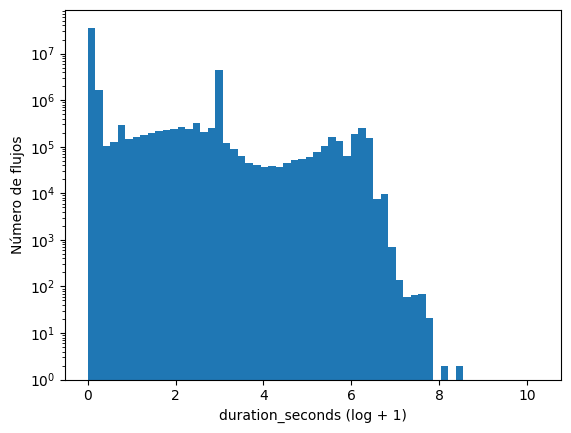
\includegraphics[width=\textwidth]{media/packet_pincer_cicddos/duration_seconds_log_x_log_y.png}
        \caption{CIC-DDoS2019}
    \end{subfigure}
    \hfill
    \begin{subfigure}[b]{0.26\textwidth}
        \centering
        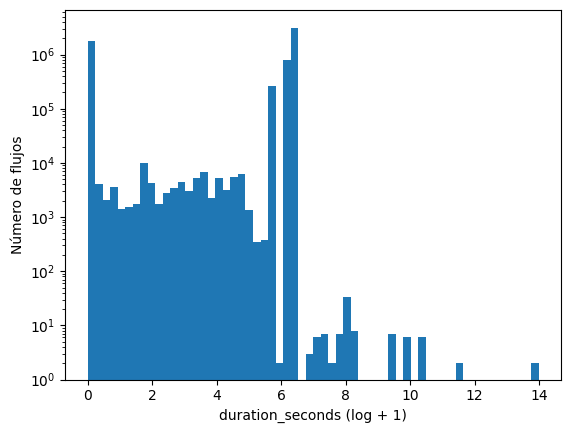
\includegraphics[width=\linewidth]{media/packet_pincer_botiot/duration_seconds_log_x_log_y.png}
        \caption{BoT-IoT}
    \end{subfigure}
    \hfill
    \begin{subfigure}[b]{0.26\textwidth}
        \centering
        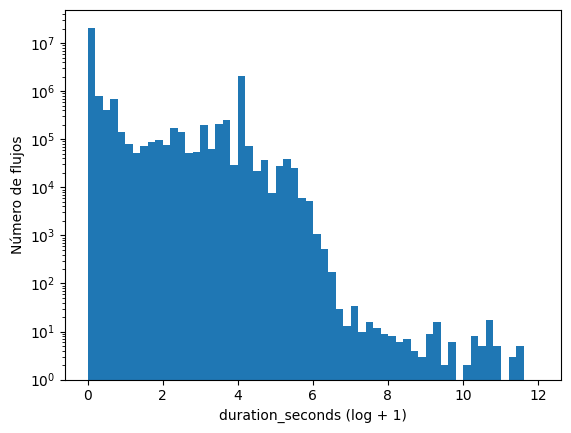
\includegraphics[width=\linewidth]{media/packet_pincer_toniot/duration_seconds_log_x_log_y.png}
        \caption{TON-IoT}
    \end{subfigure}
       \caption{Distribución de la duración de los flujos}
       \label{fig:packet_pincer_duration}
\end{figure}

\subsubsection{Recuento de paquetes}

\begin{figure}[H]
    \centering
    \hfill
    \begin{subfigure}[b]{0.26\textwidth}
        \centering
        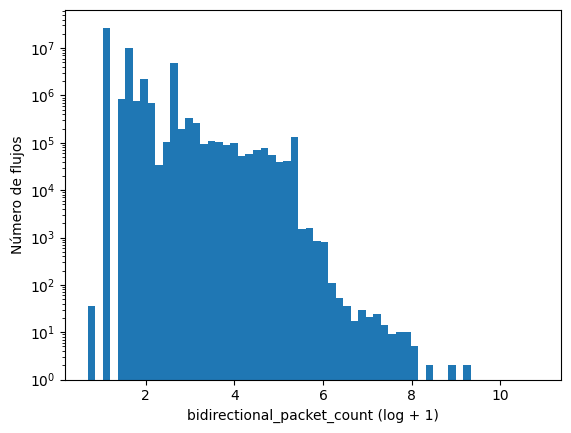
\includegraphics[width=\textwidth]{media/packet_pincer_cicddos/bidirectional_packet_count_log_x_log_y.png}
        \caption{CD (bidir.)}
        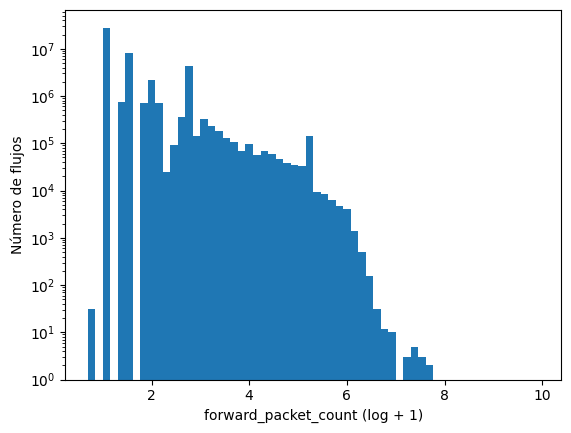
\includegraphics[width=\textwidth]{media/packet_pincer_cicddos/forward_packet_count_log_x_log_y.png}
        \caption{CD (forward)}
        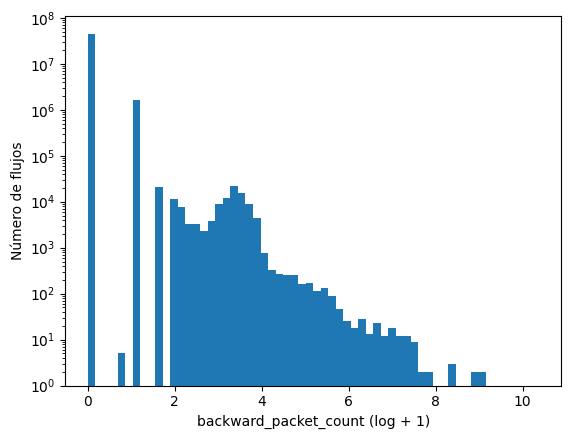
\includegraphics[width=\textwidth]{media/packet_pincer_cicddos/backward_packet_count_log_x_log_y.png}
        \caption{CD (backward)}
    \end{subfigure}
    \hfill
    \begin{subfigure}[b]{0.26\textwidth}
        \centering
        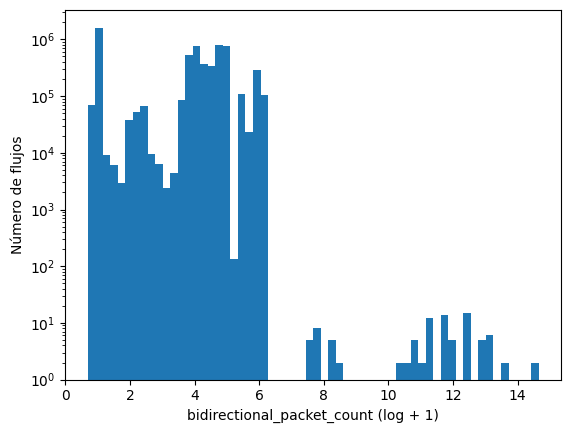
\includegraphics[width=\linewidth]{media/packet_pincer_botiot/bidirectional_packet_count_log_x_log_y.png}
        \caption{BI (bidir.)}
        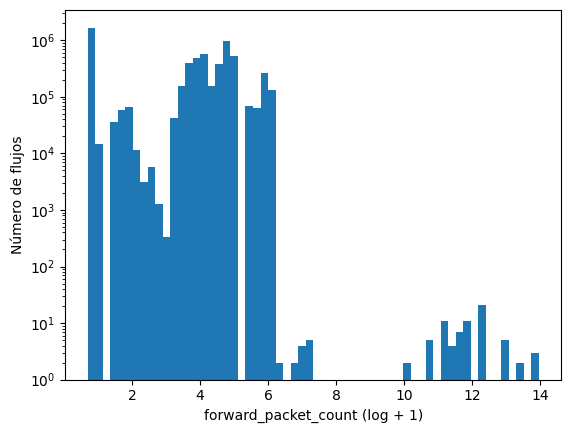
\includegraphics[width=\textwidth]{media/packet_pincer_botiot/forward_packet_count_log_x_log_y.png}
        \caption{BI (forward)}
        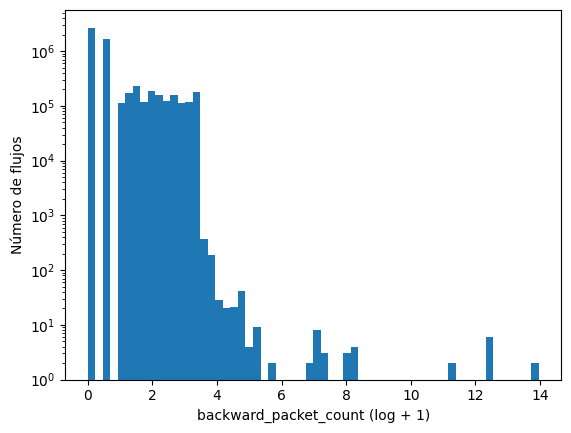
\includegraphics[width=\textwidth]{media/packet_pincer_botiot/backward_packet_count_log_x_log_y.png}
        \caption{BI (backward)}
    \end{subfigure}
    \hfill
    \begin{subfigure}[b]{0.26\textwidth}
        \centering
        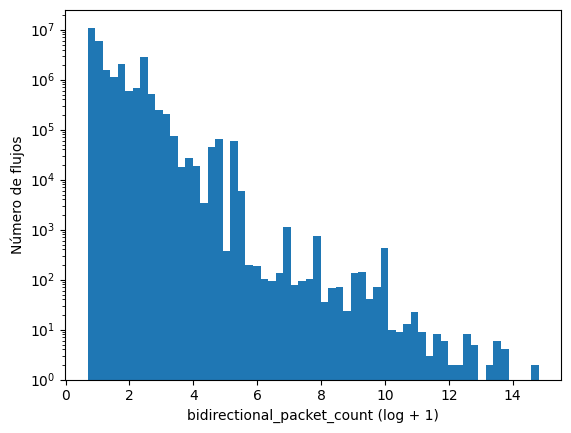
\includegraphics[width=\linewidth]{media/packet_pincer_toniot/bidirectional_packet_count_log_x_log_y.png}
        \caption{TI (bidir.)}
        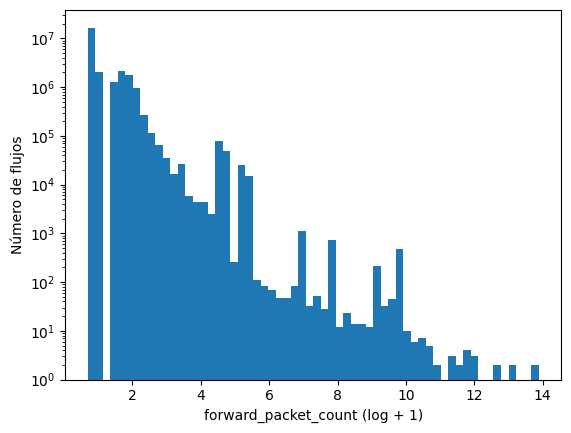
\includegraphics[width=\textwidth]{media/packet_pincer_toniot/forward_packet_count_log_x_log_y.png}
        \caption{TI (forward)}
        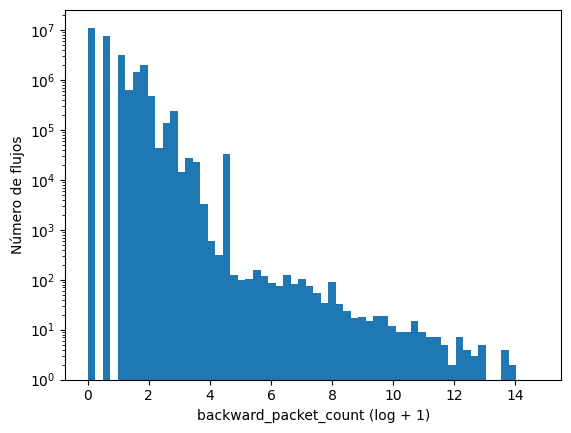
\includegraphics[width=\textwidth]{media/packet_pincer_toniot/backward_packet_count_log_x_log_y.png}
        \caption{TI (backward)}
    \end{subfigure}
    \hfill
       \caption{Distribución del número de paquetes}
       \label{fig:packet_pincer_packet_count}
\end{figure}

Podemos observar en la Figura \ref{fig:packet_pincer_packet_count} que tenemos una situación parecida al caso de la duración con el recuento de paquetes. La mayoría de los flujos tienen una cantidad de paquetes intercambiados reducida. Adicionalmente, en la mayoría hay una caída clara a partir de un punto, aunque en otros es más progresivo. Para CIC-DDoS2019 (CD en la figura) y en ToN-IoT (TI en la figura), podemos observar cierta tendencia que predice la ley de Zipf.

En este caso, para la columna del recuento de paquetes de regreso, tenemos que la cantidad de ceros es el 96.29\% (46 588 405), 44.39\% (2 697 786) y 41.71\% (11 264 084) en CIC-DDoS2019, BoT-Iot y TON-IoT, respectivamente. Las otras dos no contienen ningún cero, debido a que si fuesen cero, el flujo no aparecería en los datos procesados.

\subsubsection{Cadencia de paquetes}

\begin{figure}[H]
    \centering
    \hfill
    \begin{subfigure}[b]{0.26\textwidth}
        \centering
        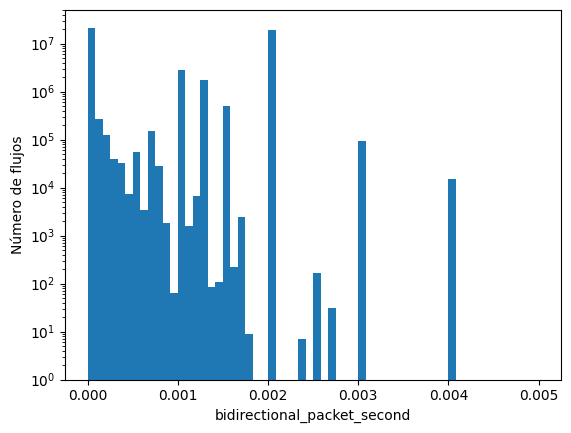
\includegraphics[width=\textwidth]{media/packet_pincer_cicddos/bidirectional_packet_second_linear_x_log_y.png}
        \caption{CD (bidir.)}
        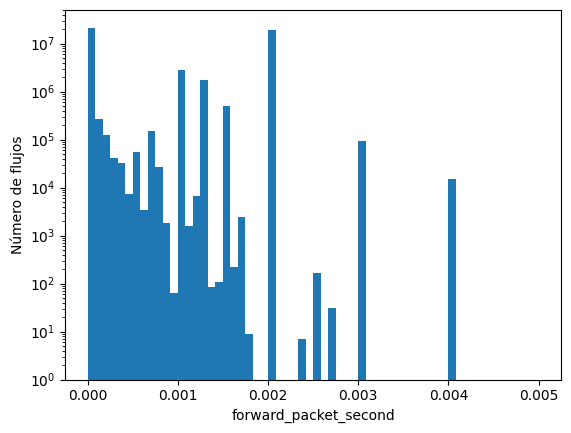
\includegraphics[width=\textwidth]{media/packet_pincer_cicddos/forward_packet_second_linear_x_log_y.png}
        \caption{CD (forward)}
        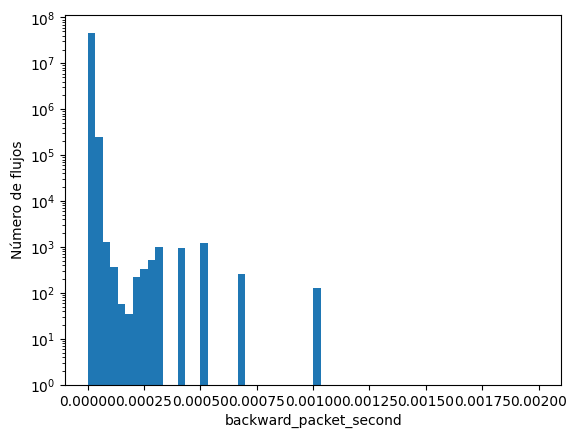
\includegraphics[width=\textwidth]{media/packet_pincer_cicddos/backward_packet_second_linear_x_log_y.png}
        \caption{CD (backward)}
    \end{subfigure}
    \hfill
    \begin{subfigure}[b]{0.26\textwidth}
        \centering
        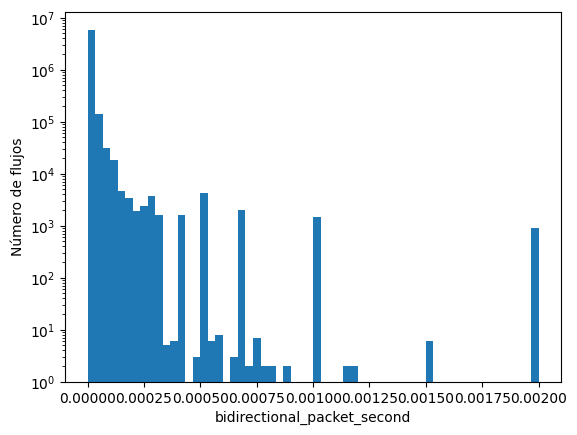
\includegraphics[width=\linewidth]{media/packet_pincer_botiot/bidirectional_packet_second_linear_x_log_y.png}
        \caption{BI (bidir.)}
        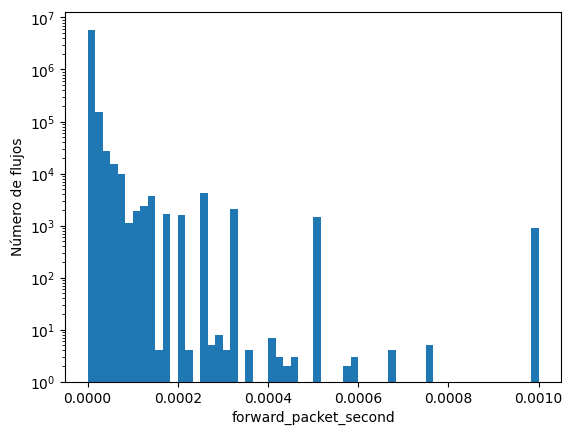
\includegraphics[width=\textwidth]{media/packet_pincer_botiot/forward_packet_second_linear_x_log_y.png}
        \caption{BI (forward)}
        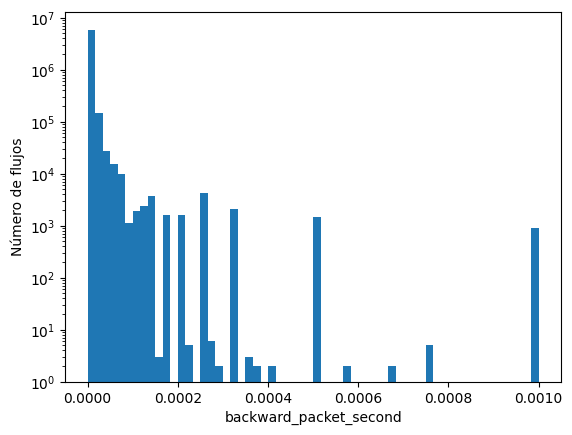
\includegraphics[width=\textwidth]{media/packet_pincer_botiot/backward_packet_second_linear_x_log_y.png}
        \caption{BI (backward)}
    \end{subfigure}
    \hfill
    \begin{subfigure}[b]{0.26\textwidth}
        \centering
        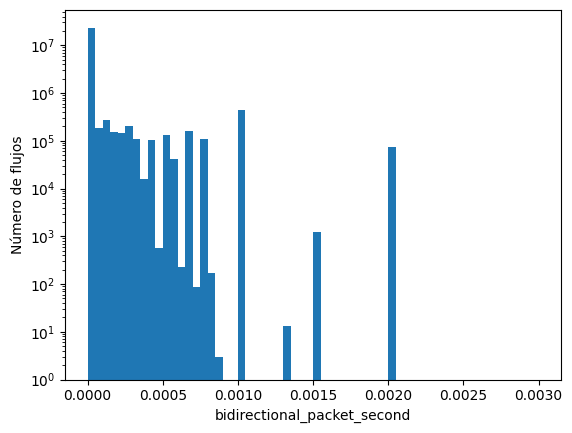
\includegraphics[width=\linewidth]{media/packet_pincer_toniot/bidirectional_packet_second_linear_x_log_y.png}
        \caption{TI (bidir.)}
        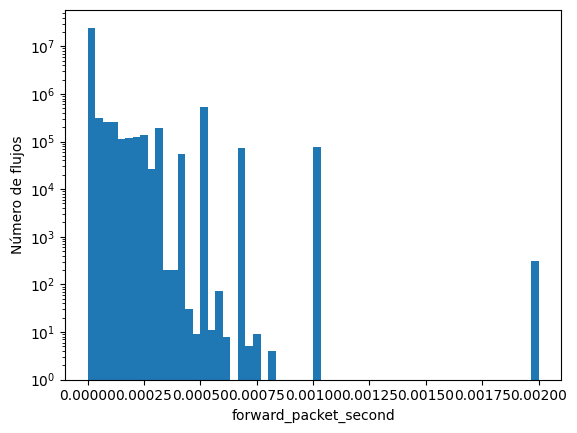
\includegraphics[width=\textwidth]{media/packet_pincer_toniot/forward_packet_second_linear_x_log_y.png}
        \caption{TI (forward)}
        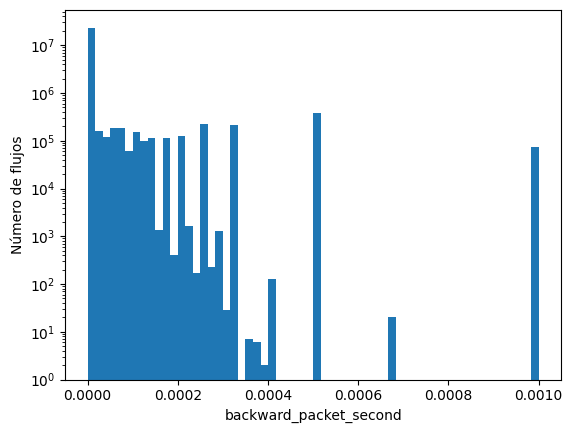
\includegraphics[width=\textwidth]{media/packet_pincer_toniot/backward_packet_second_linear_x_log_y.png}
        \caption{TI (backward)}
    \end{subfigure}
    \hfill
       \caption{Distribución de la cadencia de paquetes}
       \label{fig:packet_pincer_packet_second}
\end{figure}

La distribución de las diferentes cadencias de paquetes se puede observar en la Figura \ref{fig:packet_pincer_packet_second}. Podemos ver que la mayoría de los flujos tiene una cadencia baja, con algunos puntos con picos. En la Tabla \ref{table:packet_pincer_packet_second_zeroes} podemos ver que también hay gran cantidad de ceros en el conjunto de datos, especialmente en los IoT y en los casos de retorno. Es posible que esto haya sido debido a muchos paquetes que no hayan tenido respuesta.

\begin{table}[H]
    \centering
    \begin{tabular}{|c | c c c |}
        \hline
        \textbf{Conjunto de datos} & \textbf{Bidirectional} & \textbf{Forward} & \textbf{Backward} \\ \hline
        CIC-DDoS2019               & 6,97\%                 & 6,99\%           & 95,55\% \\
        Bot-IoT                    & 64,38\%                & 64,53\%          & 71,14\% \\
        TON-IoT                    & 53,10\%                & 54,44\%          & 55,27\% \\
        \hline
    \end{tabular}
    \caption{Protocolo de transporte utilizado por conjunto de datos}
    \label{table:packet_pincer_packet_second_zeroes}
\end{table}

\subsubsection{Número de bytes transmitidos por flujo}

\begin{figure}[H]
    \centering
    \hfill
    \begin{subfigure}[b]{0.26\textwidth}
        \centering
        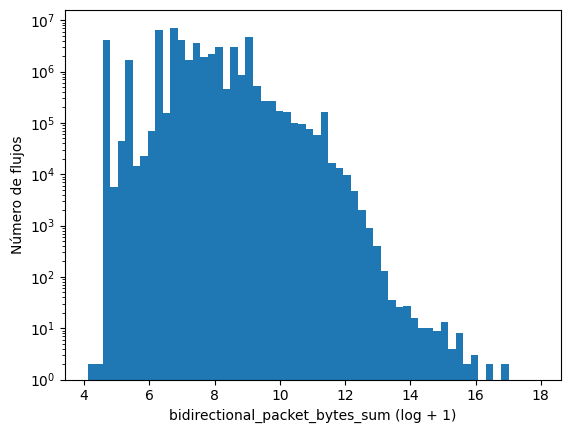
\includegraphics[width=\textwidth]{media/packet_pincer_cicddos/bidirectional_packet_bytes_sum_log_x_log_y.png}
        \caption{CD (bidir.)}
        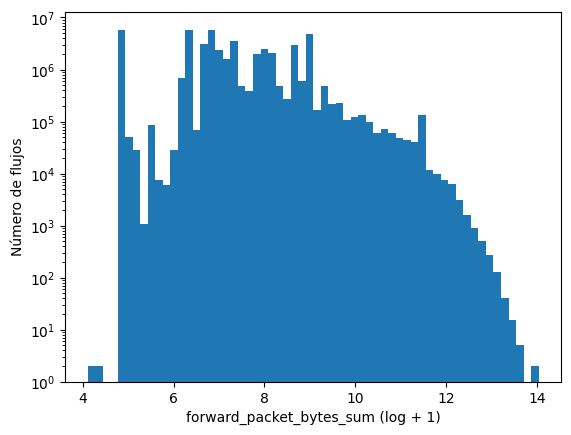
\includegraphics[width=\textwidth]{media/packet_pincer_cicddos/forward_packet_bytes_sum_log_x_log_y.png}
        \caption{CD (forward)}
        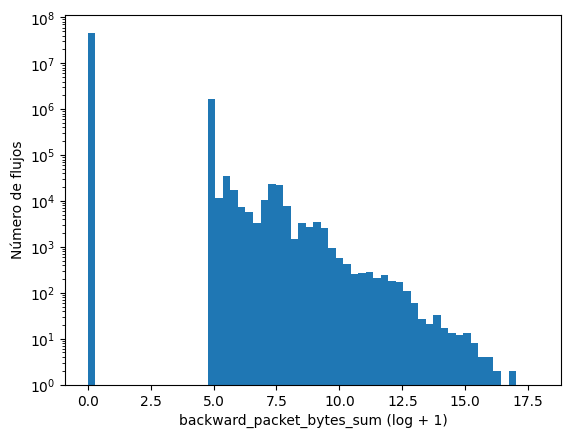
\includegraphics[width=\textwidth]{media/packet_pincer_cicddos/backward_packet_bytes_sum_log_x_log_y.png}
        \caption{CD (backward)}
    \end{subfigure}
    \hfill
    \begin{subfigure}[b]{0.26\textwidth}
        \centering
        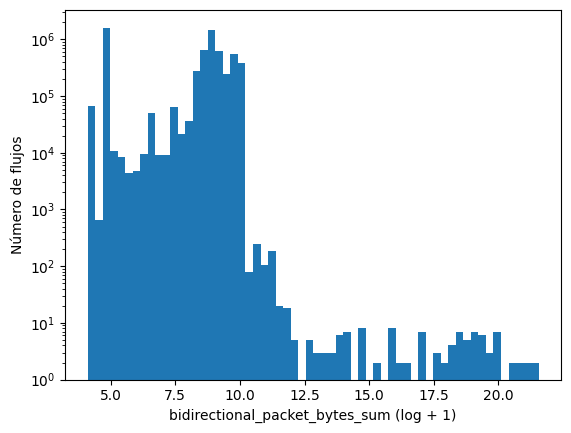
\includegraphics[width=\linewidth]{media/packet_pincer_botiot/bidirectional_packet_bytes_sum_log_x_log_y.png}
        \caption{BI (bidir.)}
        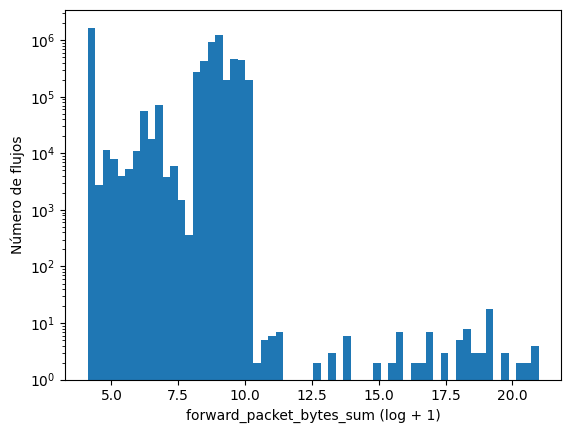
\includegraphics[width=\textwidth]{media/packet_pincer_botiot/forward_packet_bytes_sum_log_x_log_y.png}
        \caption{BI (forward)}
        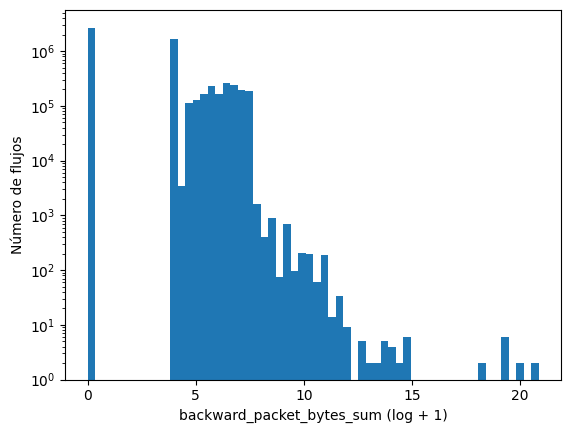
\includegraphics[width=\textwidth]{media/packet_pincer_botiot/backward_packet_bytes_sum_log_x_log_y.png}
        \caption{BI (backward)}
    \end{subfigure}
    \hfill
    \begin{subfigure}[b]{0.26\textwidth}
        \centering
        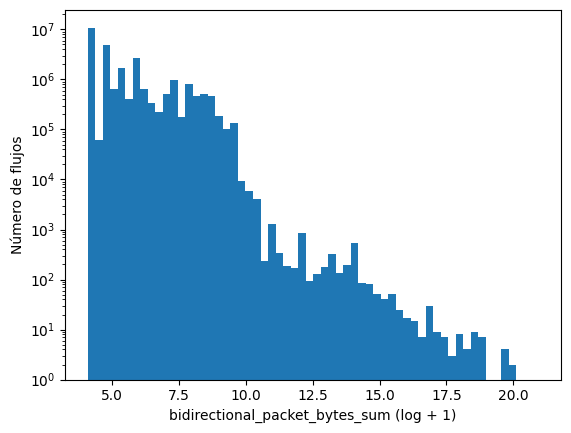
\includegraphics[width=\linewidth]{media/packet_pincer_toniot/bidirectional_packet_bytes_sum_log_x_log_y.png}
        \caption{TI (bidir.)}
        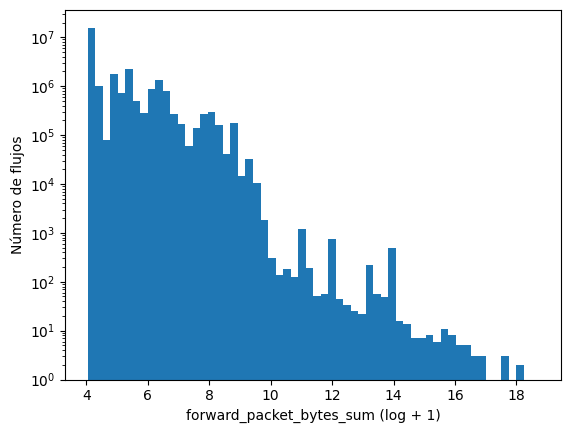
\includegraphics[width=\textwidth]{media/packet_pincer_toniot/forward_packet_bytes_sum_log_x_log_y.png}
        \caption{TI (forward)}
        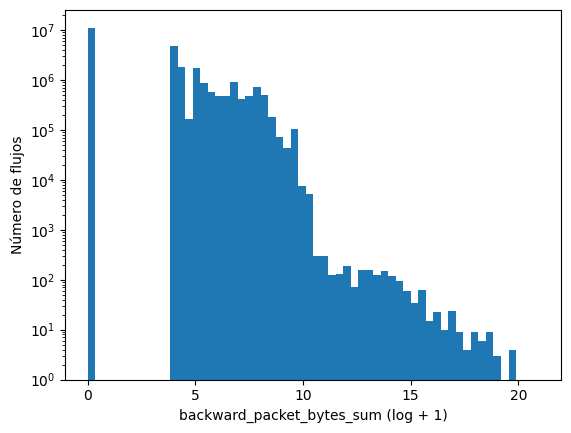
\includegraphics[width=\textwidth]{media/packet_pincer_toniot/backward_packet_bytes_sum_log_x_log_y.png}
        \caption{TI (backward)}
    \end{subfigure}
    \hfill
       \caption{Distribución de la suma de bytes transmitidas por flujo}
       \label{fig:packet_pincer_packet_bytes_sum}
\end{figure}

La distribución de las sumas totales de los bytes transmitidos por cada flujo está representada en la Figura \ref{fig:packet_pincer_packet_bytes_sum}. Podemos ver que en algunos casos la distribución parece marcada por la ley de Zipf, pero otro se asemeja más a una distribución normal al expresarlo en una gráfica log-log. Adicionalmente, en otros tenemos una caída notable a partir de cierto punto. Aparte de las peticiones que no reciben respuesta, no hay registros con ceros.

\subsubsection{Número de bytes máximos por flujo}

Si observamos las distribuciones de los bytes máximos en paquetes por flujo representadas en la Figura \ref{fig:packet_pincer_packet_bytes_max}, podemos ver que en general son similares a las del punto anterior. Sin embargo, en el caso 'backward' del conjunto de datos de CIC-DDoS2019 (subfigura \ref{fig:packet_pincer_packet_bytes_max_backward}), podemos ver cómo la 'cola' de la distribución parece haber sido cortada. Adicionalmente, los picos parecen ser menos pronunciados para los otros dos conjuntos.

\begin{figure}[H]
    \centering
    \hfill
    \begin{subfigure}[b]{0.26\textwidth}
        \centering
        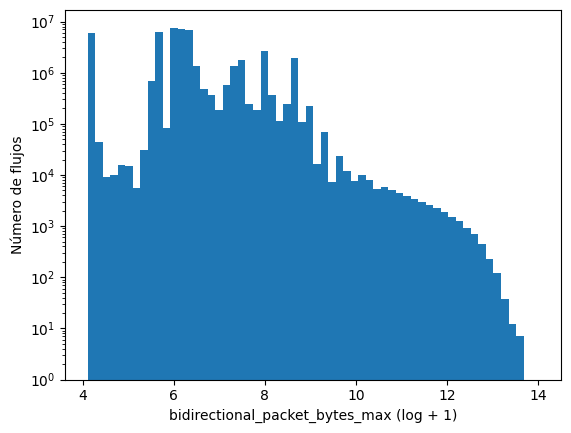
\includegraphics[width=\textwidth]{media/packet_pincer_cicddos/bidirectional_packet_bytes_max_log_x_log_y.png}
        \caption{CD (bidir.)}
        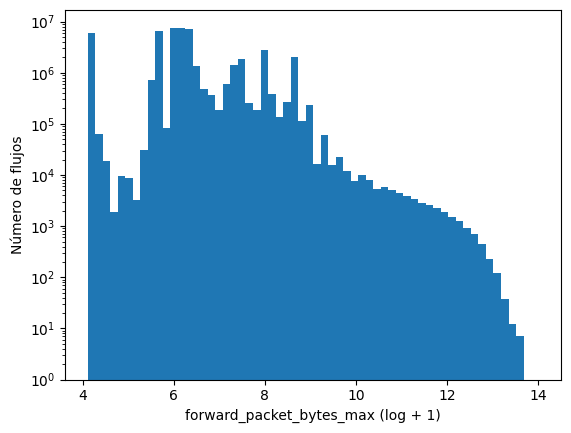
\includegraphics[width=\textwidth]{media/packet_pincer_cicddos/forward_packet_bytes_max_log_x_log_y.png}
        \caption{CD (forward)}
        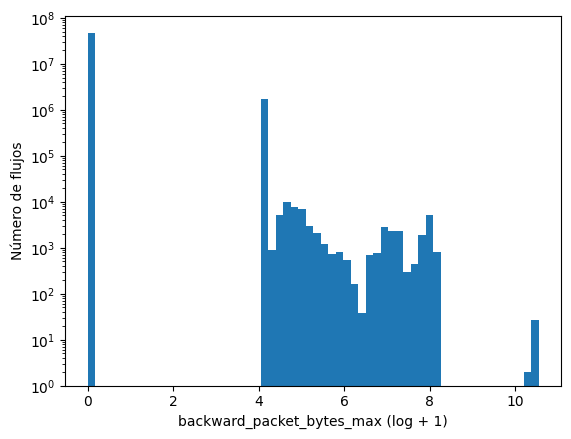
\includegraphics[width=\textwidth]{media/packet_pincer_cicddos/backward_packet_bytes_max_log_x_log_y.png}
        \caption{CD (backward)} \label{fig:packet_pincer_packet_bytes_max_backward}
    \end{subfigure}
    \hfill
    \begin{subfigure}[b]{0.26\textwidth}
        \centering
        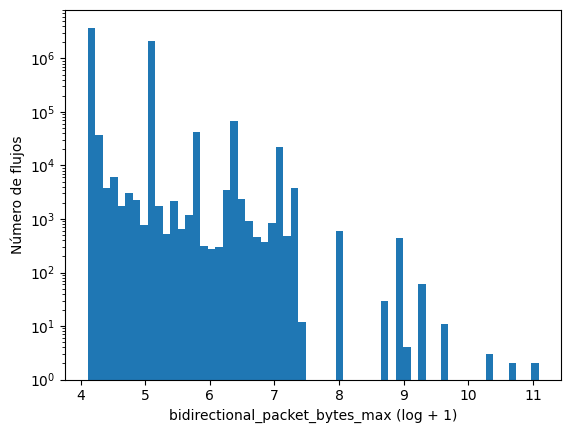
\includegraphics[width=\linewidth]{media/packet_pincer_botiot/bidirectional_packet_bytes_max_log_x_log_y.png}
        \caption{BI (bidir.)}
        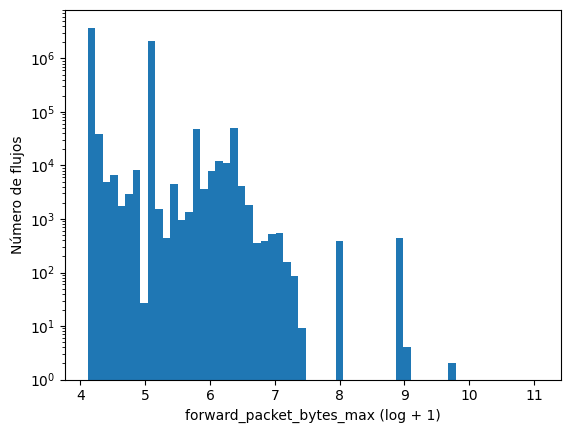
\includegraphics[width=\textwidth]{media/packet_pincer_botiot/forward_packet_bytes_max_log_x_log_y.png}
        \caption{BI (forward)}
        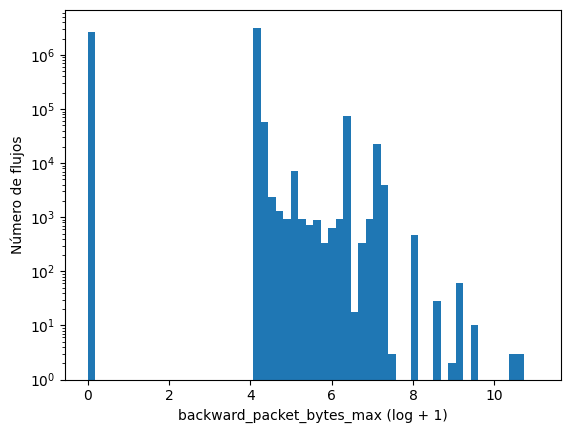
\includegraphics[width=\textwidth]{media/packet_pincer_botiot/backward_packet_bytes_max_log_x_log_y.png}
        \caption{BI (backward)}
    \end{subfigure}
    \hfill
    \begin{subfigure}[b]{0.26\textwidth}
        \centering
        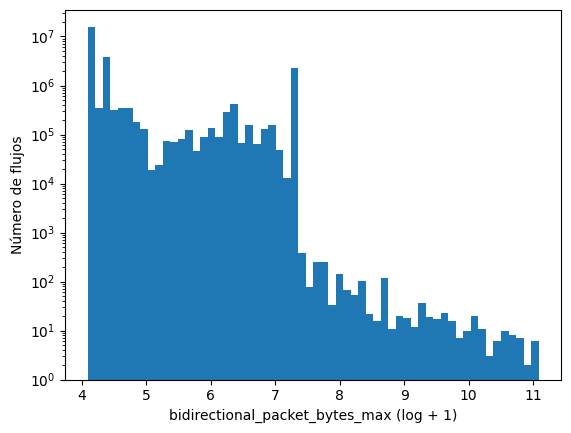
\includegraphics[width=\linewidth]{media/packet_pincer_toniot/bidirectional_packet_bytes_max_log_x_log_y.png}
        \caption{TI (bidir.)}
        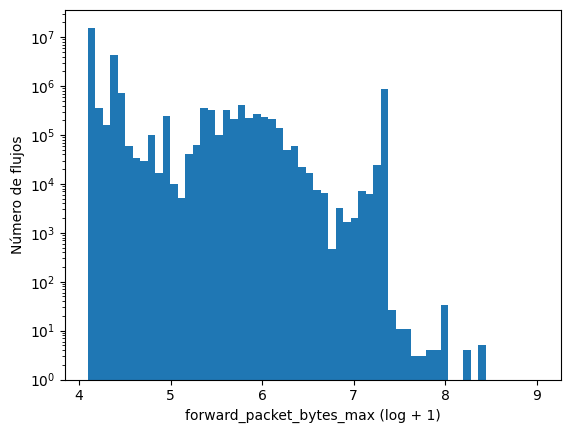
\includegraphics[width=\textwidth]{media/packet_pincer_toniot/forward_packet_bytes_max_log_x_log_y.png}
        \caption{TI (forward)}
        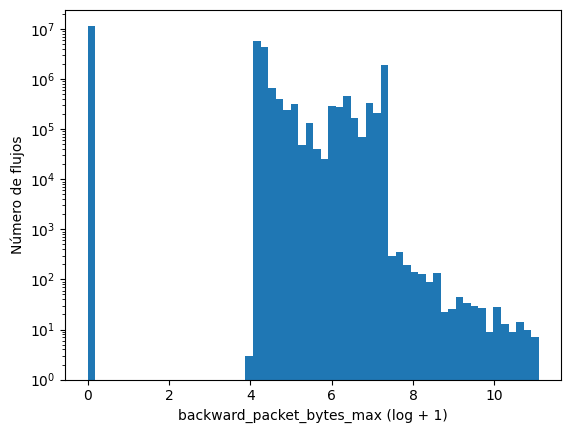
\includegraphics[width=\textwidth]{media/packet_pincer_toniot/backward_packet_bytes_max_log_x_log_y.png}
        \caption{TI (backward)}
    \end{subfigure}
    \hfill
       \caption{Distribución de los máximos bytes transmitidos en un paquete por flujo}
       \label{fig:packet_pincer_packet_bytes_max}
\end{figure}

\subsubsection{Número de bytes mínimos por flujo}

Para el caso de bytes mínimos en paquetes, podemos ver que en la Figura \ref{fig:packet_pincer_packet_bytes_min} nos encontramos con una situación al caso de los máximos. Sin embargo, para CIC-DDoS2019, el corte es en una magnitud menor (subfigura \ref{fig:packet_pincer_packet_bytes_min_backward}) y en los otros parece haber más huecos y concentraciones en ciertos puntos de la distribución.

\begin{figure}[H]
    \centering
    \hfill
    \begin{subfigure}[b]{0.26\textwidth}
        \centering
        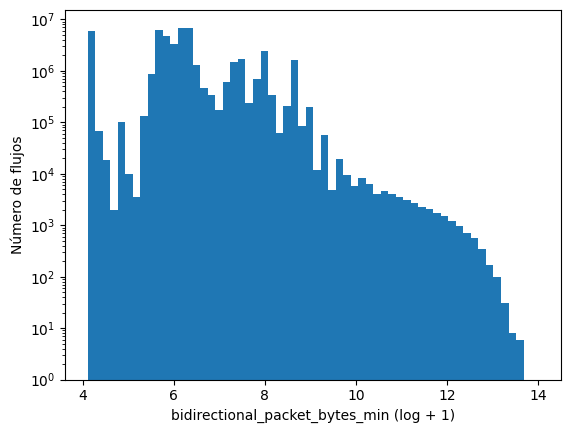
\includegraphics[width=\textwidth]{media/packet_pincer_cicddos/bidirectional_packet_bytes_min_log_x_log_y.png}
        \caption{CD (bidir.)}
        \includegraphics[width=\textwidth]{media/packet_pincer_cicddos/forward_packet_bytes_min_log_x_log_y.png}
        \caption{CD (forward)}
        \includegraphics[width=\textwidth]{media/packet_pincer_cicddos/backward_packet_bytes_min_log_x_log_y.png}
        \caption{CD (backward)} \label{fig:packet_pincer_packet_bytes_min_backward}
    \end{subfigure}
    \hfill
    \begin{subfigure}[b]{0.26\textwidth}
        \centering
        \includegraphics[width=\linewidth]{media/packet_pincer_botiot/bidirectional_packet_bytes_min_log_x_log_y.png}
        \caption{BI (bidir.)}
        \includegraphics[width=\textwidth]{media/packet_pincer_botiot/forward_packet_bytes_min_log_x_log_y.png}
        \caption{BI (forward)}
        \includegraphics[width=\textwidth]{media/packet_pincer_botiot/backward_packet_bytes_min_log_x_log_y.png}
        \caption{BI (backward)}
    \end{subfigure}
    \hfill
    \begin{subfigure}[b]{0.26\textwidth}
        \centering
        \includegraphics[width=\linewidth]{media/packet_pincer_toniot/bidirectional_packet_bytes_min_log_x_log_y.png}
        \caption{TI (bidir.)}
        \includegraphics[width=\textwidth]{media/packet_pincer_toniot/forward_packet_bytes_min_log_x_log_y.png}
        \caption{TI (forward)}
        \includegraphics[width=\textwidth]{media/packet_pincer_toniot/backward_packet_bytes_min_log_x_log_y.png}
        \caption{TI (backward)}
    \end{subfigure}
    \hfill
       \caption{Distribución de los mínimos bytes transmitidos en un paquete por flujo}
       \label{fig:packet_pincer_packet_bytes_min}
\end{figure}

\subsubsection{Número de bytes medio por flujo}

Las distribuciones de los bytes medios de la Figura \ref{fig:packet_pincer_packet_bytes_mean} se asemejan a las de los recuentos de los bytes totales, pero suavizadas. Podemos ver que, en el caso bidireccional de TON-IoT (subfigura \ref{fig:packet_pincer_packet_bytes_mean_ti_bidir}), la gráfica se mantiene en número de flujos alto durante un mayor rango de medias antes de caer.

\begin{figure}[H]
    \centering
    \hfill
    \begin{subfigure}[b]{0.26\textwidth}
        \centering
        \includegraphics[width=\textwidth]{media/packet_pincer_cicddos/bidirectional_packet_bytes_mean_log_x_log_y.png}
        \caption{CD (bidir.)}
        \includegraphics[width=\textwidth]{media/packet_pincer_cicddos/forward_packet_bytes_mean_log_x_log_y.png}
        \caption{CD (forward)}
        \includegraphics[width=\textwidth]{media/packet_pincer_cicddos/backward_packet_bytes_mean_log_x_log_y.png}
        \caption{CD (backward)}
    \end{subfigure}
    \hfill
    \begin{subfigure}[b]{0.26\textwidth}
        \centering
        \includegraphics[width=\linewidth]{media/packet_pincer_botiot/bidirectional_packet_bytes_mean_log_x_log_y.png}
        \caption{BI (bidir.)}
        \includegraphics[width=\textwidth]{media/packet_pincer_botiot/forward_packet_bytes_mean_log_x_log_y.png}
        \caption{BI (forward)}
        \includegraphics[width=\textwidth]{media/packet_pincer_botiot/backward_packet_bytes_mean_log_x_log_y.png}
        \caption{BI (backward)}
    \end{subfigure}
    \hfill
    \begin{subfigure}[b]{0.26\textwidth}
        \centering
        \includegraphics[width=\linewidth]{media/packet_pincer_toniot/bidirectional_packet_bytes_mean_log_x_log_y.png}
        \caption{TI (bidir.)} \label{fig:packet_pincer_packet_bytes_mean_ti_bidir}
        \includegraphics[width=\textwidth]{media/packet_pincer_toniot/forward_packet_bytes_mean_log_x_log_y.png}
        \caption{TI (forward)}
        \includegraphics[width=\textwidth]{media/packet_pincer_toniot/backward_packet_bytes_mean_log_x_log_y.png}
        \caption{TI (backward)}
    \end{subfigure}
    \hfill
       \caption{Distribución de los bytes medios transmitidos en un paquete por flujo}
       \label{fig:packet_pincer_packet_bytes_mean}
\end{figure}

\subsubsection{Desviación estándar del número de bytes por flujo}

Las distribuciones de las diferentes desviaciones estándar son variadas. Tenemos en muchos casos donde la desviación es 0, la cual puede ser causada por flujos con paquetes muy iguales o los casos donde no se transmite nada, ya que se asigna 0 en ese caso. De todas formas, para todos los casos, donde no son 0, hay una variedad de distribuciones. En el caso de CIC-DDoS2019, se mantiene el estilo de sus distribuciones anteriores en el caso bidireccional y hacia el receptor inicial. Para el caso hacia el transmisor inicial (subfigura \ref{fig:packet_pincer_packet_bytes_std_cd_bw}) está invertida, teniendo mucha variabilidad en la cantidad total de bytes enviados. La gran diferencia de variabilidad es quizá debido a los efectos del control de congestión de las transmisiones. Dependiendo del estado de la red, los diferentes dispositivos transmitirán de una forma más constante y predecible y en otras se tendrán que ir adaptando a tiempo real al nivel de congestión.

\begin{figure}[H]
    \centering
    \hfill
    \begin{subfigure}[b]{0.26\textwidth}
        \centering
        \includegraphics[width=\textwidth]{media/packet_pincer_cicddos/bidirectional_packet_bytes_std_log_x_log_y.png}
        \caption{CD (bidir.)}
        \includegraphics[width=\textwidth]{media/packet_pincer_cicddos/forward_packet_bytes_std_log_x_log_y.png}
        \caption{CD (forward)}
        \includegraphics[width=\textwidth]{media/packet_pincer_cicddos/backward_packet_bytes_std_log_x_log_y.png}
        \caption{CD (backward)} \label{fig:packet_pincer_packet_bytes_std_cd_bw}
    \end{subfigure}
    \hfill
    \begin{subfigure}[b]{0.26\textwidth}
        \centering
        \includegraphics[width=\linewidth]{media/packet_pincer_botiot/bidirectional_packet_bytes_std_log_x_log_y.png}
        \caption{BI (bidir.)}
        \includegraphics[width=\textwidth]{media/packet_pincer_botiot/forward_packet_bytes_std_log_x_log_y.png}
        \caption{BI (forward)}
        \includegraphics[width=\textwidth]{media/packet_pincer_botiot/backward_packet_bytes_std_log_x_log_y.png}
        \caption{BI (backward)}
    \end{subfigure}
    \hfill
    \begin{subfigure}[b]{0.26\textwidth}
        \centering
        \includegraphics[width=\linewidth]{media/packet_pincer_toniot/bidirectional_packet_bytes_std_log_x_log_y.png}
        \caption{TI (bidir.)}
        \includegraphics[width=\textwidth]{media/packet_pincer_toniot/forward_packet_bytes_std_log_x_log_y.png}
        \caption{TI (forward)}
        \includegraphics[width=\textwidth]{media/packet_pincer_toniot/backward_packet_bytes_std_log_x_log_y.png}
        \caption{TI (backward)}
    \end{subfigure}
    \hfill
       \caption{Desviación estándard del número de bytes transmitidos en un paquete por flujo}
       \label{fig:packet_pincer_packet_bytes_std}
\end{figure}

\subsubsection{Balance entre subida y bajada}

El balance o la razón entre la subida y bajada consiste en dividir la cantidad de bytes enviados por el receptor inicial entre los enviados por el iniciador de la comunicación. De esta manera, se puede inferir si la comunicación es principalmente de bajada (un valor inferior a 1), de subida (un valor superior a 1) o hay una comunicación a iguales. En el primer caso, se puede dar al visitar la web o descargar archivos. El segundo en casos donde se suban datos, como subir fotos a un servicio Cloud. Finalmente, el tercero podría consistir en, por ejemplo, en una llamada de voz o videoconferencia. 

Podemos ver en la Figura \ref{fig:packet_pincer_down_up_bytes_ratio} que la gran mayoría de comunicaciones se concentran en la parte baja del gráfico, indicando que suelen ser o de bajada o la cantidad de datos enviados no suele ser muy grande. Sin embargo, hay una cantidad relevante de flujos en la que el emisor de la comunicación envía muchos más datos de los que recibe. Esto puede estar relacionado con posibles ataques, donde las comunicaciones normales tienen un ratio más bajo.

\begin{figure}[H]
    \centering
    \begin{subfigure}[b]{0.32\textwidth}
        \centering
        \includegraphics[width=\textwidth]{media/packet_pincer_cicddos/down_up_bytes_ratio_log_x_log_y.png}
        \caption{CIC-DDoS2019}
    \end{subfigure}
    \hfill
    \begin{subfigure}[b]{0.32\textwidth}
        \centering
        \includegraphics[width=\linewidth]{media/packet_pincer_botiot/down_up_bytes_ratio_log_x_log_y.png}
        \caption{BoT-IoT}
    \end{subfigure}
    \hfill
    \begin{subfigure}[b]{0.32\textwidth}
        \centering
        \includegraphics[width=\linewidth]{media/packet_pincer_toniot/down_up_bytes_ratio_log_x_log_y.png}
        \caption{TON-IoT}
    \end{subfigure}
       \caption{Distribución del balance de los flujos}
       \label{fig:packet_pincer_down_up_bytes_ratio}
\end{figure}

\subsubsection{Cadencia de datos}

\begin{figure}[H]
    \centering
    \hfill
    \begin{subfigure}[b]{0.26\textwidth}
        \centering
        \includegraphics[width=\textwidth]{media/packet_pincer_cicddos/bidirectional_bytes_s_log_x_log_y.png}
        \caption{CD (bidir.)}
        \includegraphics[width=\textwidth]{media/packet_pincer_cicddos/forward_bytes_s_log_x_log_y.png}
        \caption{CD (forward)}
        \includegraphics[width=\textwidth]{media/packet_pincer_cicddos/backward_bytes_s_log_x_log_y.png}
        \caption{CD (backward)}
    \end{subfigure}
    \hfill
    \begin{subfigure}[b]{0.26\textwidth}
        \centering
        \includegraphics[width=\linewidth]{media/packet_pincer_botiot/bidirectional_bytes_s_log_x_log_y.png}
        \caption{BI (bidir.)}
        \includegraphics[width=\textwidth]{media/packet_pincer_botiot/forward_bytes_s_log_x_log_y.png}
        \caption{BI (forward)}
        \includegraphics[width=\textwidth]{media/packet_pincer_botiot/backward_bytes_s_log_x_log_y.png}
        \caption{BI (backward)}
    \end{subfigure}
    \hfill
    \begin{subfigure}[b]{0.26\textwidth}
        \centering
        \includegraphics[width=\linewidth]{media/packet_pincer_toniot/bidirectional_bytes_s_log_x_log_y.png}
        \caption{TI (bidir.)}
        \includegraphics[width=\textwidth]{media/packet_pincer_toniot/forward_bytes_s_log_x_log_y.png}
        \caption{TI (forward)}
        \includegraphics[width=\textwidth]{media/packet_pincer_toniot/backward_bytes_s_log_x_log_y.png}
        \caption{TI (backward)}
    \end{subfigure}
    \hfill
       \caption{Cadencia de bytes medios por flujo}
       \label{fig:packet_pincer_bytes_s}
\end{figure}

En la Figura \ref{fig:packet_pincer_bytes_s} podemos ver la distribución de las diferentes cadencias medias de bytes transmitidos por flujos. Podemos observar que hay mayor variedad en el caso de CIC-DDoS2019, mientras que en las otras los valores son más bajos y se encuentran más concentrados. Estos valores pueden aportar información sobre transmisiones en las que haya habido mayor o menor actividad.

\subsubsection{Tiempo de llegada máxima}

\begin{figure}[H]
    \centering
    \hfill
    \begin{subfigure}[b]{0.26\textwidth}
        \centering
        \includegraphics[width=\textwidth]{media/packet_pincer_cicddos/bidirectional_inter_arrival_time_max_log_x_log_y.png}
        \caption{CD (bidir.)}
        \includegraphics[width=\textwidth]{media/packet_pincer_cicddos/forward_inter_arrival_time_max_log_x_log_y.png}
        \caption{CD (forward)}
        \includegraphics[width=\textwidth]{media/packet_pincer_cicddos/backward_inter_arrival_time_max_log_x_log_y.png}
        \caption{CD (backward)}
    \end{subfigure}
    \hfill
    \begin{subfigure}[b]{0.26\textwidth}
        \centering
        \includegraphics[width=\linewidth]{media/packet_pincer_botiot/bidirectional_inter_arrival_time_max_log_x_log_y.png}
        \caption{BI (bidir.)}
        \includegraphics[width=\textwidth]{media/packet_pincer_botiot/forward_inter_arrival_time_max_log_x_log_y.png}
        \caption{BI (forward)}
        \includegraphics[width=\textwidth]{media/packet_pincer_botiot/backward_inter_arrival_time_max_log_x_log_y.png}
        \caption{BI (backward)}
    \end{subfigure}
    \hfill
    \begin{subfigure}[b]{0.26\textwidth}
        \centering
        \includegraphics[width=\linewidth]{media/packet_pincer_toniot/bidirectional_inter_arrival_time_max_log_x_log_y.png}
        \caption{TI (bidir.)}
        \includegraphics[width=\textwidth]{media/packet_pincer_toniot/forward_inter_arrival_time_max_log_x_log_y.png}
        \caption{TI (forward)}
        \includegraphics[width=\textwidth]{media/packet_pincer_toniot/backward_inter_arrival_time_max_log_x_log_y.png}
        \caption{TI (backward)}
    \end{subfigure}
    \hfill
       \caption{Distribución del tiempo de llegada máxima entre paquetes}
       \label{fig:packet_pincer_inter_arrival_time_max}
\end{figure}

La distribución de los tiempos de llegada máxima entre paquetes la podemos observar en la Figura \ref{fig:packet_pincer_inter_arrival_time_max}. Podemos ver que en los casos de CIC-DDoS2019 y TON-IOT, aparte de los ceros, la distribución de tiempos se encuentra relativamente repartida. En cambio, en BoT-IoT hay una acumulación clara en cierto punto de la gráfica.

\subsubsection{Tiempo de llegada mínima}

\begin{figure}[H]
    \centering
    \hfill
    \begin{subfigure}[b]{0.26\textwidth}
        \centering
        \includegraphics[width=\textwidth]{media/packet_pincer_cicddos/bidirectional_inter_arrival_time_min_log_x_log_y.png}
        \caption{CD (bidir.)}
        \includegraphics[width=\textwidth]{media/packet_pincer_cicddos/forward_inter_arrival_time_min_log_x_log_y.png}
        \caption{CD (forward)}
        \includegraphics[width=\textwidth]{media/packet_pincer_cicddos/backward_inter_arrival_time_min_log_x_log_y.png}
        \caption{CD (backward)}
    \end{subfigure}
    \hfill
    \begin{subfigure}[b]{0.26\textwidth}
        \centering
        \includegraphics[width=\linewidth]{media/packet_pincer_botiot/bidirectional_inter_arrival_time_min_log_x_log_y.png}
        \caption{BI (bidir.)}
        \includegraphics[width=\textwidth]{media/packet_pincer_botiot/forward_inter_arrival_time_min_log_x_log_y.png}
        \caption{BI (forward)}
        \includegraphics[width=\textwidth]{media/packet_pincer_botiot/backward_inter_arrival_time_min_log_x_log_y.png}
        \caption{BI (backward)} \label{fig:packet_pincer_inter_arrival_time_min_bi_min}
    \end{subfigure}
    \hfill
    \begin{subfigure}[b]{0.26\textwidth}
        \centering
        \includegraphics[width=\linewidth]{media/packet_pincer_toniot/bidirectional_inter_arrival_time_min_log_x_log_y.png}
        \caption{TI (bidir.)}
        \includegraphics[width=\textwidth]{media/packet_pincer_toniot/forward_inter_arrival_time_min_log_x_log_y.png}
        \caption{TI (forward)}
        \includegraphics[width=\textwidth]{media/packet_pincer_toniot/backward_inter_arrival_time_min_log_x_log_y.png}
        \caption{TI (backward)}
    \end{subfigure}
    \hfill
       \caption{Distribución del tiempo de llegada mínima entre paquetes}
       \label{fig:packet_pincer_inter_arrival_time_min}
\end{figure}

Para el caso de las llegadas mínimas entre paquetes, como podemos ver en la Figura \ref{fig:packet_pincer_inter_arrival_time_min}, tenemos que las distribuciones en BoT-Iot y TON-IoT son similares. Sin embargo, sin contar los ceros, en CIC-DDoS2019 tenemos que el caso bidireccional y hacia el receptor inicial tenemos mayor cantidad en la parte alta. Adicionalmente, con BoT-IoT no tenemos el mismo pico en para el caso 'backwards' (subfigura \ref{fig:packet_pincer_inter_arrival_time_min_bi_min})

\subsubsection{Tiempo de llegada media}

Si observamos las distribuciones del tiempo de llegada media de la Figura \ref{fig:packet_pincer_inter_arrival_time_mean}, sin tener en cuenta los ceros, podemos observar que en general hay bastante variedad entre los diferentes flujos. De todas maneras, en el caso de BoT-IoT hay mayor agrupación en la parte baja en el caso bidireccional y hacia el receptor inicial.

\begin{figure}[H]
    \centering
    \hfill
    \begin{subfigure}[b]{0.32\textwidth}
        \centering
        \includegraphics[width=\textwidth]{media/packet_pincer_cicddos/bidirectional_inter_arrival_time_mean_log_x_log_y.png}
        \caption{CD (bidir.)}
        \includegraphics[width=\textwidth]{media/packet_pincer_cicddos/forward_inter_arrival_time_mean_log_x_log_y.png}
        \caption{CD (forward)}
        \includegraphics[width=\textwidth]{media/packet_pincer_cicddos/backward_inter_arrival_time_mean_log_x_log_y.png}
        \caption{CD (backward)}
    \end{subfigure}
    \hfill
    \begin{subfigure}[b]{0.32\textwidth}
        \centering
        \includegraphics[width=\linewidth]{media/packet_pincer_botiot/bidirectional_inter_arrival_time_mean_log_x_log_y.png}
        \caption{BI (bidir.)}
        \includegraphics[width=\textwidth]{media/packet_pincer_botiot/forward_inter_arrival_time_mean_log_x_log_y.png}
        \caption{BI (forward)}
        \includegraphics[width=\textwidth]{media/packet_pincer_botiot/backward_inter_arrival_time_mean_log_x_log_y.png}
        \caption{BI (backward)}
    \end{subfigure}
    \hfill
    \begin{subfigure}[b]{0.32\textwidth}
        \centering
        \includegraphics[width=\linewidth]{media/packet_pincer_toniot/bidirectional_inter_arrival_time_mean_log_x_log_y.png}
        \caption{TI (bidir.)}
        \includegraphics[width=\textwidth]{media/packet_pincer_toniot/forward_inter_arrival_time_mean_log_x_log_y.png}
        \caption{TI (forward)}
        \includegraphics[width=\textwidth]{media/packet_pincer_toniot/backward_inter_arrival_time_mean_log_x_log_y.png}
        \caption{TI (backward)}
    \end{subfigure}
    \hfill
       \caption{Distribución de la media del tiempo de llegada entre paquetes}
       \label{fig:packet_pincer_inter_arrival_time_mean}
\end{figure}

\subsubsection{Desviación estándar de los tiempos de llegada}

Para el caso de la desviación estándar, tenemos un caso parecido a las medias como podemos ver en la figura \ref{fig:packet_pincer_inter_arrival_time_std}. De todas maneras, las magnitudes son algo menores y la distribución está más desplazadas hacia la izquierda. 

Este valor puede aportar información como en otros casos de la situación de la congestión de la red y caracterizar mejor el flujo en cuestión. Si los tiempos de llegada varían mucho, puede ser señal de una conexión inestable o, en caso de ser un ataque, sobre el intentar aparentar tener una conexión inestable para consumir recursos del sistema receptor.

\begin{figure}[H]
    \centering
    \hfill
    \begin{subfigure}[b]{0.26\textwidth}
        \centering
        \includegraphics[width=\textwidth]{media/packet_pincer_cicddos/bidirectional_inter_arrival_time_std_log_x_log_y.png}
        \caption{CD (bidir.)}
        \includegraphics[width=\textwidth]{media/packet_pincer_cicddos/forward_inter_arrival_time_std_log_x_log_y.png}
        \caption{CD (forward)}
        \includegraphics[width=\textwidth]{media/packet_pincer_cicddos/backward_inter_arrival_time_std_log_x_log_y.png}
        \caption{CD (backward)}
    \end{subfigure}
    \hfill
    \begin{subfigure}[b]{0.26\textwidth}
        \centering
        \includegraphics[width=\linewidth]{media/packet_pincer_botiot/bidirectional_inter_arrival_time_std_log_x_log_y.png}
        \caption{BI (bidir.)}
        \includegraphics[width=\textwidth]{media/packet_pincer_botiot/forward_inter_arrival_time_std_log_x_log_y.png}
        \caption{BI (forward)}
        \includegraphics[width=\textwidth]{media/packet_pincer_botiot/backward_inter_arrival_time_std_log_x_log_y.png}
        \caption{BI (backward)}
    \end{subfigure}
    \hfill
    \begin{subfigure}[b]{0.26\textwidth}
        \centering
        \includegraphics[width=\linewidth]{media/packet_pincer_toniot/bidirectional_inter_arrival_time_std_log_x_log_y.png}
        \caption{TI (bidir.)}
        \includegraphics[width=\textwidth]{media/packet_pincer_toniot/forward_inter_arrival_time_std_log_x_log_y.png}
        \caption{TI (forward)}
        \includegraphics[width=\textwidth]{media/packet_pincer_toniot/backward_inter_arrival_time_std_log_x_log_y.png}
        \caption{TI (backward)}
    \end{subfigure}
    \hfill
       \caption{Distribución de las distribuciones estándar del tiempo de llegada}
       \label{fig:packet_pincer_inter_arrival_time_std}
\end{figure}

\subsubsection{Flags CWR, ECE y URG en cabecera TCP}

Podemos ver en Figura \ref{fig:packet_pincer_bidirectional_tcp_cwr_flags_count}, Figura \ref{fig:packet_pincer_bidirectional_tcp_ece_flags_count} y Figura \ref{fig:packet_pincer_bidirectional_tcp_urg_flags_count} que apenas tenemos flujos que tengan las flags CWR, ECE o URG activas.

\begin{figure}[H]
    \centering
    \begin{subfigure}[b]{0.32\textwidth}
        \centering
        \includegraphics[width=\textwidth]{media/packet_pincer_cicddos/bidirectional_tcp_cwr_flags_count_linear_x_log_y.png}
        \caption{CIC-DDoS2019}
    \end{subfigure}
    \hfill
    \begin{subfigure}[b]{0.32\textwidth}
        \centering
        \includegraphics[width=\linewidth]{media/packet_pincer_botiot/bidirectional_tcp_cwr_flags_count_linear_x_log_y.png}
        \caption{BoT-IoT}
    \end{subfigure}
    \hfill
    \begin{subfigure}[b]{0.32\textwidth}
        \centering
        \includegraphics[width=\linewidth]{media/packet_pincer_toniot/bidirectional_tcp_cwr_flags_count_linear_x_log_y.png}
        \caption{TON-IoT}
    \end{subfigure}
       \caption{Distribución de recuentos de paquetes con la flag CWR en TCP activa}
       \label{fig:packet_pincer_bidirectional_tcp_cwr_flags_count}
\end{figure}

\begin{figure}[H]
    \centering
    \begin{subfigure}[b]{0.32\textwidth}
        \centering
        \includegraphics[width=\textwidth]{media/packet_pincer_cicddos/bidirectional_tcp_ece_flags_count_linear_x_log_y.png}
        \caption{CIC-DDoS2019}
    \end{subfigure}
    \hfill
    \begin{subfigure}[b]{0.32\textwidth}
        \centering
        \includegraphics[width=\linewidth]{media/packet_pincer_botiot/bidirectional_tcp_ece_flags_count_linear_x_log_y.png}
        \caption{BoT-IoT}
    \end{subfigure}
    \hfill
    \begin{subfigure}[b]{0.32\textwidth}
        \centering
        \includegraphics[width=\linewidth]{media/packet_pincer_toniot/bidirectional_tcp_ece_flags_count_linear_x_log_y.png}
        \caption{TON-IoT}
    \end{subfigure}
       \caption{Distribución de recuentos de paquetes con la flag ECE en TCP activa}
       \label{fig:packet_pincer_bidirectional_tcp_ece_flags_count}
\end{figure}

\begin{figure}[H]
    \centering
    \begin{subfigure}[b]{0.32\textwidth}
        \centering
        \includegraphics[width=\textwidth]{media/packet_pincer_cicddos/bidirectional_tcp_urg_flags_count_linear_x_log_y.png}
        \caption{CIC-DDoS2019}
    \end{subfigure}
    \hfill
    \begin{subfigure}[b]{0.32\textwidth}
        \centering
        \includegraphics[width=\linewidth]{media/packet_pincer_botiot/bidirectional_tcp_urg_flags_count_linear_x_log_y.png}
        \caption{BoT-IoT}
    \end{subfigure}
    \hfill
    \begin{subfigure}[b]{0.32\textwidth}
        \centering
        \includegraphics[width=\linewidth]{media/packet_pincer_toniot/bidirectional_tcp_urg_flags_count_linear_x_log_y.png}
        \caption{TON-IoT}
    \end{subfigure}
       \caption{Distribución de recuentos de paquetes con la flag URG en TCP activa}
       \label{fig:packet_pincer_bidirectional_tcp_urg_flags_count}
\end{figure}

\subsubsection{Flags ACK en cabecera TCP}

\begin{figure}[H]
    \centering
    \begin{subfigure}[b]{0.32\textwidth}
        \centering
        \includegraphics[width=\textwidth]{media/packet_pincer_cicddos/bidirectional_tcp_ack_flags_count_log_x_log_y.png}
        \caption{CIC-DDoS2019}
    \end{subfigure}
    \hfill
    \begin{subfigure}[b]{0.32\textwidth}
        \centering
        \includegraphics[width=\linewidth]{media/packet_pincer_botiot/bidirectional_tcp_ack_flags_count_log_x_log_y.png}
        \caption{BoT-IoT}
    \end{subfigure}
    \hfill
    \begin{subfigure}[b]{0.32\textwidth}
        \centering
        \includegraphics[width=\linewidth]{media/packet_pincer_toniot/bidirectional_tcp_ack_flags_count_log_x_log_y.png}
        \caption{TON-IoT}
    \end{subfigure}
       \caption{Distribución de recuentos de paquetes con la flag ACK en TCP activa}
       \label{fig:packet_pincer_bidirectional_tcp_ack_flags_count}
\end{figure}

En una transmisión TCP, ambos nodos han de confirmar los datos que han recibido para que el otro pueda saber que puede enviar los siguientes. Si una conexión que debería tener más validaciones de recepción no las tiene, es posible que nos encontremos delante de un ataque. En la Figura \ref{fig:packet_pincer_bidirectional_tcp_ack_flags_count} podemos ver que los diferentes datasets tienen una forma similar, con algunos teniendo la caída antes que otros.

\subsubsection{Flags PSH en cabecera TCP}

\begin{figure}[H]
    \centering
    \begin{subfigure}[b]{0.26\textwidth}
        \centering
        \includegraphics[width=\textwidth]{media/packet_pincer_cicddos/bidirectional_tcp_psh_flags_count_log_x_log_y.png}
        \caption{CD (bidir.)}
        \includegraphics[width=\textwidth]{media/packet_pincer_cicddos/forward_tcp_psh_flags_count_log_x_log_y.png}
        \caption{CD (forward)}
        \includegraphics[width=\textwidth]{media/packet_pincer_cicddos/backward_tcp_psh_flags_count_log_x_log_y.png}
        \caption{CD (backward)}
    \end{subfigure}
    \hfill
    \begin{subfigure}[b]{0.26\textwidth}
        \centering
        \includegraphics[width=\linewidth]{media/packet_pincer_botiot/bidirectional_tcp_psh_flags_count_log_x_log_y.png}
        \caption{BI (bidir.)}
        \includegraphics[width=\linewidth]{media/packet_pincer_botiot/forward_tcp_psh_flags_count_log_x_log_y.png}
        \caption{BI (forward)}
        \includegraphics[width=\linewidth]{media/packet_pincer_botiot/backward_tcp_psh_flags_count_log_x_log_y.png}
        \caption{BI (backward)}
    \end{subfigure}
    \hfill
    \begin{subfigure}[b]{0.26\textwidth}
        \centering
        \includegraphics[width=\linewidth]{media/packet_pincer_toniot/bidirectional_tcp_psh_flags_count_log_x_log_y.png}
        \caption{TI (bidir.)}
        \includegraphics[width=\linewidth]{media/packet_pincer_toniot/forward_tcp_psh_flags_count_log_x_log_y.png}
        \caption{TI (forward)}
        \includegraphics[width=\linewidth]{media/packet_pincer_toniot/backward_tcp_psh_flags_count_log_x_log_y.png}
        \caption{TI (backward)}
    \end{subfigure}
       \caption{Distribución de recuentos de paquetes con la flag PSH en TCP activa}
       \label{fig:packet_pincer_bidirectional_tcp_psh_flags_count}
\end{figure}

La flag PSH en las cabeceras TCP, como se indicó en una sección anterior, son utilizadas para indicar al código que gestiona la capa de transporte que proporcione los datos enviados lo antes posible a la capa de aplicación. Como se puede observar en la Figura \ref{fig:packet_pincer_bidirectional_tcp_psh_flags_count}, una gran cantidad de flujos no la utilizan. Sin embargo, también hay cierta cantidad que si lo hace, y en las gráficas log-log podemos ver como en general va decreciendo. En algunos casos es progresivo, pero en otros la caída es más notable.

\subsubsection{Flags RST en cabecera TCP}

\begin{figure}[H]
    \centering
    \hfill
    \begin{subfigure}[b]{0.32\textwidth}
        \centering
        \includegraphics[width=\textwidth]{media/packet_pincer_cicddos/bidirectional_tcp_rst_flags_count_linear_x_log_y.png}
        \includegraphics[width=\textwidth]{media/packet_pincer_cicddos/bidirectional_tcp_rst_flags_count_log_x_log_y.png}
        \caption{CIC-DDoS2019}
    \end{subfigure}
    \hfill
    \begin{subfigure}[b]{0.32\textwidth}
        \centering
        \includegraphics[width=\linewidth]{media/packet_pincer_botiot/bidirectional_tcp_rst_flags_count_linear_x_log_y.png}
        \includegraphics[width=\linewidth]{media/packet_pincer_botiot/bidirectional_tcp_rst_flags_count_log_x_log_y.png}
        \caption{BoT-IoT}
    \end{subfigure}
    \hfill
    \begin{subfigure}[b]{0.32\textwidth}
        \centering
        \includegraphics[width=\linewidth]{media/packet_pincer_toniot/bidirectional_tcp_rst_flags_count_linear_x_log_y.png}
        \includegraphics[width=\linewidth]{media/packet_pincer_toniot/bidirectional_tcp_rst_flags_count_log_x_log_y.png}
        \caption{TON-IoT}
    \end{subfigure}
    \hfill
       \caption{Distribución de recuentos de paquetes con la flag RST en TCP activa}
       \label{fig:packet_pincer_bidirectional_tcp_rst_flags_count}
\end{figure}

Los flags RST provocan una finalización de la conexión más precipitada, fuerzan al iniciador de la conexión a volver a empezar la sincronización TCP inicial. En el mejor caso no se utiliza, pero como se puede observar en la Figura \ref{fig:packet_pincer_bidirectional_tcp_rst_flags_count}, tenemos ejemplos donde si se hace uso. Podemos ver que en CIC-DDoS2019 y BoT-IoT, aun utilizando un eje x lineal (arriba) hay mucha variedad de flujos donde se utiliza, pero en TON-IoT hace falta tener la gráfica con el eje x en formato logarítmico (abajo) para poder observar más de tres columnas en el histograma. Es posible que esto haya sido debido a que en los dos primeros, se hagan ciertos ataques que hagan mal uso de este campo de la cabecera, mientras que en el tercero no.

\subsubsection{Flags FIN en cabecera TCP}

Las flags FIN en comunicaciones TCP suele haber 2, si se finaliza correctamente la comunicación o ninguna si no lo hace. En caso de haber más, puede ser señal de que un ataque está ocurriendo. En la Figura \ref{fig:packet_pincer_bidirectional_tcp_fin_flags_count} podemos comprobar que la mayoría de flujos no tienen, pero hay otros que superan las 2 y llegan a tener hasta 20.

\begin{figure}[H]
    \centering
    \begin{subfigure}[b]{0.32\textwidth}
        \centering
        \includegraphics[width=\textwidth]{media/packet_pincer_cicddos/bidirectional_tcp_fin_flags_count_linear_x_log_y.png}
        \includegraphics[width=\textwidth]{media/packet_pincer_cicddos/bidirectional_tcp_fin_flags_count_log_x_log_y.png}
        \caption{CIC-DDoS2019}
    \end{subfigure}
    \hfill
    \begin{subfigure}[b]{0.32\textwidth}
        \centering
        \includegraphics[width=\linewidth]{media/packet_pincer_botiot/bidirectional_tcp_fin_flags_count_linear_x_log_y.png}
        \includegraphics[width=\linewidth]{media/packet_pincer_botiot/bidirectional_tcp_fin_flags_count_log_x_log_y.png}
        \caption{BoT-IoT}
    \end{subfigure}
    \hfill
    \begin{subfigure}[b]{0.32\textwidth}
        \centering
        \includegraphics[width=\linewidth]{media/packet_pincer_toniot/bidirectional_tcp_fin_flags_count_linear_x_log_y.png}
        \includegraphics[width=\linewidth]{media/packet_pincer_toniot/bidirectional_tcp_fin_flags_count_log_x_log_y.png}
        \caption{TON-IoT}
    \end{subfigure}
       \caption{Distribución de recuentos de paquetes con la flag FIN en TCP activa}
       \label{fig:packet_pincer_bidirectional_tcp_fin_flags_count}
\end{figure}

\subsubsection{Suma total de bytes en las cabeceras de transporte}

\begin{figure}[H]
    \centering
    \begin{subfigure}[b]{0.26\textwidth}
        \centering
        \includegraphics[width=\textwidth]{media/packet_pincer_cicddos/forward_transport_header_bytes_sum_log_x_log_y.png}
        \caption{CD (forward)}
        \includegraphics[width=\textwidth]{media/packet_pincer_cicddos/backward_transport_header_bytes_sum_log_x_log_y.png}
        \caption{CD (backward)}
    \end{subfigure}
    \hfill
    \begin{subfigure}[b]{0.26\textwidth}
        \centering
        \includegraphics[width=\linewidth]{media/packet_pincer_botiot/forward_transport_header_bytes_sum_log_x_log_y.png}
        \caption{BI (forward)}
        \includegraphics[width=\linewidth]{media/packet_pincer_botiot/backward_transport_header_bytes_sum_log_x_log_y.png}
        \caption{BI (backward)}
    \end{subfigure}
    \hfill
    \begin{subfigure}[b]{0.26\textwidth}
        \centering
        \includegraphics[width=\linewidth]{media/packet_pincer_toniot/forward_transport_header_bytes_sum_log_x_log_y.png}
        \caption{TI (forward)}
        \includegraphics[width=\linewidth]{media/packet_pincer_toniot/backward_transport_header_bytes_sum_log_x_log_y.png}
        \caption{TI (backward)}
    \end{subfigure}
       \caption{Distribución de las sumas totales en las cabeceras de transporte}
       \label{fig:packet_pincer_bidirectional_transport_header_bytes_sum}
\end{figure}

La columna de las sumas totales de las cabeceras de transporte se generó debido a que aparecía en CICFlowMeter. Si observamos las distribuciones de la Figura \ref{fig:packet_pincer_bidirectional_transport_header_bytes_sum}, podemos ver que son similares al caso de la suma general. Hay ciertas variaciones, pero es posible que esté muy correlacionado y no aporte suficiente información adicional.

\subsubsection{Media de bytes enviados sobre la capa de transporte por paquete}

\begin{figure}[H]
    \centering
    \begin{subfigure}[b]{0.26\textwidth}
        \centering
        \includegraphics[width=\textwidth]{media/packet_pincer_cicddos/forward_transport_payload_bytes_mean_log_x_log_y.png}
        \caption{CD (forward)}
        \includegraphics[width=\textwidth]{media/packet_pincer_cicddos/backward_transport_payload_bytes_mean_log_x_log_y.png}
        \caption{CD (backward)}
    \end{subfigure}
    \hfill
    \begin{subfigure}[b]{0.26\textwidth}
        \centering
        \includegraphics[width=\linewidth]{media/packet_pincer_botiot/forward_transport_payload_bytes_mean_log_x_log_y.png}
        \caption{BI (forward)}
        \includegraphics[width=\linewidth]{media/packet_pincer_botiot/backward_transport_payload_bytes_mean_log_x_log_y.png}
        \caption{BI (backward)}
    \end{subfigure}
    \hfill
    \begin{subfigure}[b]{0.26\textwidth}
        \centering
        \includegraphics[width=\linewidth]{media/packet_pincer_toniot/forward_transport_payload_bytes_mean_log_x_log_y.png}
        \caption{TI (forward)}
        \includegraphics[width=\linewidth]{media/packet_pincer_toniot/backward_transport_payload_bytes_mean_log_x_log_y.png}
        \caption{TI (backward)}
    \end{subfigure}
       \caption{Distribución de las medias de bytes en la capa de transporte por paquete}
       \label{fig:packet_pincer_bidirectional_transport_payload_bytes_mean}
\end{figure}

La media de bytes enviados sobre la capa de transporte está en parte relacionada con la media de bytes total. Como podemos ver en la Figura \ref{fig:packet_pincer_bidirectional_transport_payload_bytes_mean}, hay cierta similitud en parte del gráfico. De todas maneras, es posible que la diferencia entre estos dos sea relevante. Por ejemplo, un atacante puede iniciar y mantener conexiones sin enviar datos, provocando que el receptor tenga recursos asignados a esta conexión de los cuales no hace uso.

\subsubsection{Bytes mínimos enviados sobre la capa de transporte hacia el receptor inicial}

\begin{figure}[H]
    \centering
    \begin{subfigure}[b]{0.32\textwidth}
        \centering
        \includegraphics[width=\textwidth]{media/packet_pincer_cicddos/forward_transport_payload_bytes_min_log_x_log_y.png}
        \caption{CD (forward)}
    \end{subfigure}
    \hfill
    \begin{subfigure}[b]{0.32\textwidth}
        \centering
        \includegraphics[width=\linewidth]{media/packet_pincer_botiot/forward_transport_payload_bytes_min_log_x_log_y.png}
        \caption{BI (forward)}
    \end{subfigure}
    \hfill
    \begin{subfigure}[b]{0.32\textwidth}
        \centering
        \includegraphics[width=\linewidth]{media/packet_pincer_toniot/forward_transport_payload_bytes_min_log_x_log_y.png}
        \caption{TI (forward)}
    \end{subfigure}
       \caption{Distribución de los bytes mímimos enviados en un paquete sobre la capa de transporte hacia el recpetor inicial}
       \label{fig:packet_pincer_forward_transport_payload_bytes_min}
\end{figure}

En el caso de los bytes mínimos sobre la capa de transporte, las distribuciones tienen mayores diferencias, como se puede ver en la Figura \ref{fig:packet_pincer_forward_transport_payload_bytes_min}. De todas maneras, la densidad es parecida, teniendo huecos parecidos en la distribución en BoT-IOT. La situación es similar a lo anterior, puede que no aporte información adicional tener la columna con el número total de bytes. Sin embargo, la diferencia en cierta manera podría proporcionar información útil.

\subsubsection{Número de paquetes con datos enviados en la capa de transporte hacia el receptor inicial}

Los protocolos de transporte suelen enviar paquetes con datos, excepto en la fase inicial de sincronización TCP. En algunos casos, pueden enviar paquetes vacíos para indicarse mutuamente que siguen estando disponibles y que la conexión se ha de mantener. Sin embargo, un atacante podría estar enviando muchos paquetes vacíos para colapsar un receptor que asume que los paquetes deberían contener datos. El receptor reservaría recursos para gestionar los paquetes, los cuales se desperdiciarían, ya que no contienen datos.

En la Figura \ref{fig:packet_pincer_forward_transport_packets_with_payload_count} podemos ver la distribución del recuento. Cada conjunto de datos presenta una distribución distinta, con un rango de magnitudes distinta.

\begin{figure}[H]
    \centering
    \begin{subfigure}[b]{0.32\textwidth}
        \centering
        \includegraphics[width=\textwidth]{media/packet_pincer_cicddos/forward_transport_packets_with_payload_count_log_x_log_y.png}
        \caption{CD (forward)}
    \end{subfigure}
    \hfill
    \begin{subfigure}[b]{0.32\textwidth}
        \centering
        \includegraphics[width=\linewidth]{media/packet_pincer_botiot/forward_transport_packets_with_payload_count_log_x_log_y.png}
        \caption{BI (forward)}
    \end{subfigure}
    \hfill
    \begin{subfigure}[b]{0.32\textwidth}
        \centering
        \includegraphics[width=\linewidth]{media/packet_pincer_toniot/forward_transport_packets_with_payload_count_log_x_log_y.png}
        \caption{TI (forward)}
    \end{subfigure}
       \caption{Distribución del número de paquetes enviados con datos en la capa de transporte hacia el receptor inicial}
       \label{fig:packet_pincer_forward_transport_packets_with_payload_count}
\end{figure}
\subsubsection{Ventana TCP inicial}

\begin{figure}[H]
    \centering
    \begin{subfigure}[b]{0.26\textwidth}
        \centering
        \includegraphics[width=\textwidth]{media/packet_pincer_cicddos/forward_tcp_initial_window_bytes_log_x_log_y.png}
        \caption{CD (forward)}
        \includegraphics[width=\textwidth]{media/packet_pincer_cicddos/backward_tcp_initial_window_bytes_log_x_log_y.png}
        \caption{CD (backward)}
    \end{subfigure}
    \hfill
    \begin{subfigure}[b]{0.26\textwidth}
        \centering
        \includegraphics[width=\linewidth]{media/packet_pincer_botiot/forward_tcp_initial_window_bytes_log_x_log_y.png}
        \caption{BI (forward)}
        \includegraphics[width=\linewidth]{media/packet_pincer_botiot/backward_tcp_initial_window_bytes_log_x_log_y.png}
        \caption{BI (backward)}
    \end{subfigure}
    \hfill
    \begin{subfigure}[b]{0.26\textwidth}
        \centering
        \includegraphics[width=\linewidth]{media/packet_pincer_toniot/forward_tcp_initial_window_bytes_log_x_log_y.png}
        \caption{TI (forward)}
        \includegraphics[width=\linewidth]{media/packet_pincer_toniot/backward_tcp_initial_window_bytes_log_x_log_y.png}
        \caption{TI (backward)}
    \end{subfigure}
       \caption{Distribución del tamaño de la ventanas TCP iniciales}
       \label{fig:packet_pincer_bidirectional_tcp_initial_window_bytes}
\end{figure}

En una comunicación TCP, las ventanas iniciales suelen ser reducidas. Conforme se progresa en la comunicación y se comprueba que la red no se encuentra saturada, son incrementadas progresivamente. Conocer la ventana inicial propuesta por el iniciador de la transmisión y su contraposición con la del receptor inicial, nos puede indicar si el iniciador está utilizando ventanas desproporcionadamente pequeñas o grandes. En la Figura \ref{fig:packet_pincer_bidirectional_tcp_initial_window_bytes} podemos ver las diferentes ventanas utilizadas. Podemos ver que en general hay algunas ventanas más comunes, aunque en TON-IoT las ventanas propuestas tienen mucha más variedad que en los otros casos.

\subsubsection{Tiempos de actividad mínimos}

Los tiempos de actividad mínimos nos pueden ayudar a ver si en un flujo la comunicación está siendo anormalmente lenta. En la Figura \ref{fig:packet_pincer_active_seconds_min} podemos ver como los tiempos activos e inactivos tienen distribuciones distintas. En el caso de CICDDoS2019 tenemos que los tiempos mínimos de actividad más grandes son menos frecuentes, mientras que los inactivos se mantienen relativamente plano. En BoT-IoT, tenemos que donde tenemos un valle en el caso activo, tenemos un pico en el caso inactivo. Finalmente, TON-IoT es una situación más exagerada, donde hay una caída más rápida para el caso activo, en el caso inactivo se mantiene más plano. Esto es esperable, ya que los dispositivos IoT que tratan de emular no están transmitiendo constantemente, sino que suelen enviar datos infrecuentemente para ahorrar batería.

\begin{figure}[H]
    \centering
    \begin{subfigure}[b]{0.26\textwidth}
        \centering
        \includegraphics[width=\textwidth]{media/packet_pincer_cicddos/active_seconds_min_log_x_log_y.png}
        \caption{CD (active)}
        \includegraphics[width=\textwidth]{media/packet_pincer_cicddos/idle_seconds_min_log_x_log_y.png}
        \caption{CD (idle)}
    \end{subfigure}
    \hfill
    \begin{subfigure}[b]{0.26\textwidth}
        \centering
        \includegraphics[width=\linewidth]{media/packet_pincer_botiot/active_seconds_min_log_x_log_y.png}
        \caption{BI (active)}
        \includegraphics[width=\linewidth]{media/packet_pincer_botiot/idle_seconds_min_log_x_log_y.png}
        \caption{BI (idle)}
    \end{subfigure}
    \hfill
    \begin{subfigure}[b]{0.26\textwidth}
        \centering
        \includegraphics[width=\linewidth]{media/packet_pincer_toniot/active_seconds_min_log_x_log_y.png}
        \caption{TI (active)}
        \includegraphics[width=\linewidth]{media/packet_pincer_toniot/idle_seconds_min_log_x_log_y.png}
        \caption{TI (idle)}
    \end{subfigure}
       \caption{Distribución de los tiempos de actividad mínimos}
       \label{fig:packet_pincer_active_seconds_min}
\end{figure}

\subsubsection{Tiempos de actividad máximos}

Las distribuciones para los tiempos de actividad máximos, como podemos ver en la Figura \ref{fig:packet_pincer_active_seconds_max}, tienen una forma similar para los casos de CICDDoS2019 y TON-IoT. Para BoT-IOT, ya no tenemos el pico y el valle claros, sino que en el caso activo desciende más rápidamente y en el caso inactivo está más distribuido y hay un valle menos pronunciado.

\begin{figure}[H]
    \centering
    \begin{subfigure}[b]{0.26\textwidth}
        \centering
        \includegraphics[width=\textwidth]{media/packet_pincer_cicddos/active_seconds_max_log_x_log_y.png}
        \caption{CD (active)}
        \includegraphics[width=\textwidth]{media/packet_pincer_cicddos/idle_seconds_max_log_x_log_y.png}
        \caption{CD (idle)}
    \end{subfigure}
    \hfill
    \begin{subfigure}[b]{0.26\textwidth}
        \centering
        \includegraphics[width=\linewidth]{media/packet_pincer_botiot/active_seconds_max_log_x_log_y.png}
        \caption{BI (active)}
        \includegraphics[width=\linewidth]{media/packet_pincer_botiot/idle_seconds_max_log_x_log_y.png}
        \caption{BI (idle)}
    \end{subfigure}
    \hfill
    \begin{subfigure}[b]{0.26\textwidth}
        \centering
        \includegraphics[width=\linewidth]{media/packet_pincer_toniot/active_seconds_max_log_x_log_y.png}
        \caption{TI (active)}
        \includegraphics[width=\linewidth]{media/packet_pincer_toniot/idle_seconds_max_log_x_log_y.png}
        \caption{TI (idle)}
    \end{subfigure}
       \caption{Distribución de los tiempos de actividad máximos}
       \label{fig:packet_pincer_active_seconds_max}
\end{figure}

\subsubsection{Tiempos de actividad medios}

\begin{figure}[H]
    \centering
    \begin{subfigure}[b]{0.26\textwidth}
        \centering
        \includegraphics[width=\textwidth]{media/packet_pincer_cicddos/active_seconds_mean_log_x_log_y.png}
        \caption{CD (active)}
        \includegraphics[width=\textwidth]{media/packet_pincer_cicddos/idle_seconds_mean_log_x_log_y.png}
        \caption{CD (idle)}
    \end{subfigure}
    \hfill
    \begin{subfigure}[b]{0.26\textwidth}
        \centering
        \includegraphics[width=\linewidth]{media/packet_pincer_botiot/active_seconds_mean_log_x_log_y.png}
        \caption{BI (active)}
        \includegraphics[width=\linewidth]{media/packet_pincer_botiot/idle_seconds_mean_log_x_log_y.png}
        \caption{BI (idle)}
    \end{subfigure}
    \hfill
    \begin{subfigure}[b]{0.26\textwidth}
        \centering
        \includegraphics[width=\linewidth]{media/packet_pincer_toniot/active_seconds_mean_log_x_log_y.png}
        \caption{TI (active)}
        \includegraphics[width=\linewidth]{media/packet_pincer_toniot/idle_seconds_mean_log_x_log_y.png}
        \caption{TI (idle)}
    \end{subfigure}
       \caption{Distribución de los tiempos de actividad medios}
       \label{fig:packet_pincer_active_seconds_mean}
\end{figure}

Para los tiempos de actividad medios, podemos ver en la Figura \ref{fig:packet_pincer_active_seconds_mean} una situación similar a los dos puntos anteriores. Para el CICDDoS2019 y TON-IoT la distribución se mantiene, pero para BoT-IOT el caso activo es similar a los máximos y el caso inactivo a los mínimos.

\subsubsection{Desviación estándar de los tiempos de actividad}

\begin{figure}[H]
    \centering
    \begin{subfigure}[b]{0.26\textwidth}
        \centering
        \includegraphics[width=\textwidth]{media/packet_pincer_cicddos/active_seconds_std_log_x_log_y.png}
        \caption{CD (active)}
        \includegraphics[width=\textwidth]{media/packet_pincer_cicddos/idle_seconds_std_log_x_log_y.png}
        \caption{CD (idle)}
    \end{subfigure}
    \hfill
    \begin{subfigure}[b]{0.26\textwidth}
        \centering
        \includegraphics[width=\linewidth]{media/packet_pincer_botiot/active_seconds_std_log_x_log_y.png}
        \caption{BI (active)}
        \includegraphics[width=\linewidth]{media/packet_pincer_botiot/idle_seconds_std_log_x_log_y.png}
        \caption{BI (idle)}
    \end{subfigure}
    \hfill
    \begin{subfigure}[b]{0.26\textwidth}
        \centering
        \includegraphics[width=\linewidth]{media/packet_pincer_toniot/active_seconds_std_log_x_log_y.png}
        \caption{TI (active)}
        \includegraphics[width=\linewidth]{media/packet_pincer_toniot/idle_seconds_std_log_x_log_y.png}
        \caption{TI (idle)}
    \end{subfigure}
       \caption{Distribución de las desviaciones estándar del tiempo de actividad}
       \label{fig:packet_pincer_active_seconds_std}
\end{figure}

Como en otros casos, podemos ver en la Figura \ref{fig:packet_pincer_active_seconds_std} como la desviación estándar no se contiene en un rango más restringido. Esto es esperable, ya que dependiendo de las condiciones de red pueden hacer que los paquetes lleguen antes o después, se reordenen o se pierdan. Dependiendo de la comunicación, si esta variabilidad no es acotada, puede ser un problema para los dispositivos. Esto puede ser potencialmente utilizada por agentes mal intencionados que traten de atacar a los sistemas.

\subsubsection{Media de paquetes por grupo activo}

Debido a que nos hemos basado en las características de CICFlowMeter para definir las utilizadas en packet\_pincer, se han creado las que indican información de grupos activos. En el caso de la cantidad de paquetes enviados en un grupo activo, podemos ver en la Figura \ref{fig:packet_pincer_active_group_packet_average} que las distribuciones tienen similitud al recuento total de paquetes. Sin embargo, existen diferencias debido a la diferencia de número de flujos activos por cada flujo. Es posible que esta información permita saber si, por ejemplo, un host está enviando una cantidad de paquetes al mismo tiempo desproporcionadamente grande o pequeña.

\begin{figure}[H]
    \centering
    \begin{subfigure}[b]{0.26\textwidth}
        \centering
        \includegraphics[width=\textwidth]{media/packet_pincer_cicddos/active_group_forward_packet_average_log_x_log_y.png}
        \caption{CD (forward)}
        \includegraphics[width=\textwidth]{media/packet_pincer_cicddos/active_group_backward_packet_average_log_x_log_y.png}
        \caption{CD (backward)}
    \end{subfigure}
    \hfill
    \begin{subfigure}[b]{0.26\textwidth}
        \centering
        \includegraphics[width=\linewidth]{media/packet_pincer_botiot/active_group_forward_packet_average_log_x_log_y.png}
        \caption{BI (forward)}
        \includegraphics[width=\linewidth]{media/packet_pincer_botiot/active_group_backward_packet_average_log_x_log_y.png}
        \caption{BI (backward)}
    \end{subfigure}
    \hfill
    \begin{subfigure}[b]{0.26\textwidth}
        \centering
        \includegraphics[width=\linewidth]{media/packet_pincer_toniot/active_group_forward_packet_average_log_x_log_y.png}
        \caption{TI (forward)}
        \includegraphics[width=\linewidth]{media/packet_pincer_toniot/active_group_backward_packet_average_log_x_log_y.png}
        \caption{TI (backward)}
    \end{subfigure}
       \caption{Distribución de la media de paquetes por grupo activo}
       \label{fig:packet_pincer_active_group_packet_average}
\end{figure}

\subsubsection{Media de bytes por grupo activo}

\begin{figure}[H]
    \centering
    \begin{subfigure}[b]{0.26\textwidth}
        \centering
        \includegraphics[width=\textwidth]{media/packet_pincer_cicddos/active_group_forward_byte_average_log_x_log_y.png}
        \caption{CD (forward)}
        \includegraphics[width=\textwidth]{media/packet_pincer_cicddos/active_group_backward_byte_average_log_x_log_y.png}
        \caption{CD (backward)}
    \end{subfigure}
    \hfill
    \begin{subfigure}[b]{0.26\textwidth}
        \centering
        \includegraphics[width=\linewidth]{media/packet_pincer_botiot/active_group_forward_byte_average_log_x_log_y.png}
        \caption{BI (forward)}
        \includegraphics[width=\linewidth]{media/packet_pincer_botiot/active_group_backward_byte_average_log_x_log_y.png}
        \caption{BI (backward)}
    \end{subfigure}
    \hfill
    \begin{subfigure}[b]{0.26\textwidth}
        \centering
        \includegraphics[width=\linewidth]{media/packet_pincer_toniot/active_group_forward_byte_average_log_x_log_y.png}
        \caption{TI (forward)}
        \includegraphics[width=\linewidth]{media/packet_pincer_toniot/active_group_backward_byte_average_log_x_log_y.png}
        \caption{TI (backward)}
    \end{subfigure}
       \caption{Distribución de la media de bytes por grupo activo}
       \label{fig:packet_pincer_active_group_byte_average}
\end{figure}

Para el caso de la media bytes por grupo activo, podemos ver en la Figura \ref{fig:packet_pincer_active_group_byte_average} que tenemos una situación similar. Las distribuciones son similares a la suma total, pero tienen algunos detalles distintos.

\subsubsection{Cadencia de bytes por grupo activo}

\begin{figure}[H]
    \centering
    \begin{subfigure}[b]{0.26\textwidth}
        \centering
        \includegraphics[width=\textwidth]{media/packet_pincer_cicddos/active_group_forward_byte_second_average_log_x_log_y.png}
        \caption{CD (forward)}
        \includegraphics[width=\textwidth]{media/packet_pincer_cicddos/active_group_backward_byte_second_average_log_x_log_y.png}
        \caption{CD (backward)}
    \end{subfigure}
    \hfill
    \begin{subfigure}[b]{0.26\textwidth}
        \centering
        \includegraphics[width=\linewidth]{media/packet_pincer_botiot/active_group_forward_byte_second_average_log_x_log_y.png}
        \caption{BI (forward)}
        \includegraphics[width=\linewidth]{media/packet_pincer_botiot/active_group_backward_byte_second_average_log_x_log_y.png}
        \caption{BI (backward)}
    \end{subfigure}
    \hfill
    \begin{subfigure}[b]{0.26\textwidth}
        \centering
        \includegraphics[width=\linewidth]{media/packet_pincer_toniot/active_group_forward_byte_second_average_log_x_log_y.png}
        \caption{TI (forward)}
        \includegraphics[width=\linewidth]{media/packet_pincer_toniot/active_group_backward_byte_second_average_log_x_log_y.png}
        \caption{TI (backward)}
    \end{subfigure}
       \caption{Distribución de la cadencia de bytes por grupo activo}
       \label{fig:packet_pincer_active_group_byte_second_average}
\end{figure}

A diferencia de los dos casos anteriores, podemos ver en la Figura \ref{fig:packet_pincer_active_group_byte_second_average} como la distribución de la cadencia de bytes media por grupo activo no es similar al caso general. Este valor nos puede llegar a aportar una mayor información, ya que representa la cantidad de información que se suele enviar cada vez que el flujo es activo.

\subsection{Definición de la tarea a realizar}

Una vez hecho un análisis inicial de los datos, podemos ver que tenemos un conjunto de datos muy desbalanceado, tanto en etiquetas como en campos donde solo hay valores en ciertos casos. Como vimos en la Tabla \ref{table:packetpincerassignedlabels}, tenemos solo un 0,846\% de ejemplos de tráfico benigno y una serie de etiquetas con diferentes niveles de especificidad. Concentradas mayoritariamente en ataques de denegación de servicio distribuido. 

La tarea de ML que realizaremos consistirá en clasificar un flujo determinado en benigno o maligno. Debido a que la mayoría de tráfico maligno es 'ddos', los modelos estarán posiblemente sesgados hacia este tipo en comparación a otros. Sin embargo, esto no supone un problema, ya que en entornos reales este tipo de ataques es uno de los más comunes que existen \cite{topciberattacks}.

\subsection{Preprocesamiento}

En el preprocesamiento inicial, se ha tomado cada archivo CSV generado por la herramienta y se leen todos los registros de flujos que hayan sido etiquetados correctamente. A continuación, se han remplazado todas las etiquetas de ataques específicos por 'malign', realizado un muestreo estratificado del 0.5\% de los datos y descartado las columnas identificativas. Con esto, de los 80 millones de filas, nos quedamos con 385 778, 382 334 de las cuales son muestras malignas y 3 444 benignas.

Una vez tomada la muestra, se ha aplicado el logaritmo sobre las características continúas sumando 1 para evitar infinitos y a continuación se han escalado todos los datos continuos para que estén en el rango $[0, 1]$. Después del escalado, se ha ejecutado una implementación del algoritmo Boruta \cite{borutapy} para realizar una selección de características más representativas. Al ejecutarlo, nos ha descartado las características del recuento de paquetes con los flags CWR, ECC y URG en las cabeceras TCP. Esto es esperable, ya que la extensa mayoría de estas eran 0.

Finalmente, se ha hecho un split 70/20/10 para entrenar los modelos, seleccionar el que tenga mejor rendimiento y comprobar la capacidad de generalización del modelo seleccionado con datos que aún no ha visto. 

\subsection{Entrenamiento de modelos}

En este subpunto se muestran los resultados de utilizar algoritmos de \gls{ml} con los datos que hemos preparado. En los casos que se puedan configurar hiperparámetros, se ha hecho una búsqueda en cuadrícula de diferentes valores y se han escogido los que presentan la mejor métrica de  'f-score macro' ofrecido por \texttt{scikit-learn}. Esta es una media aritmética entre los f-score de cada etiqueta que el modelo puede seleccionar, en nuestro caso 'benign' y 'malign'.

\subsubsection{Naive bayes}

Naive Bayes, como se define en la documentación de scikit-learn \cite{sklearnnaivebayes}, son un conjunto de algoritmos basados en el teorema de Bayes con la suposición 'naive' o inocente de que todas las características son independientes. Esta suposición no es correcta en nuestros datos, pero aun no cumpliéndose el rendimiento del algoritmo es a veces efectivo. Adicionalmente, es un modelo muy rápido de entrenar, por lo cual nos puede servir como modelo básico de referencia para comparar con los otros modelos. 

En las primeras pruebas, este modelo era el que mejor funcionaba, cosa que fue una indicación de que había algo incorrecto en los datos. Inicialmente, se había hecho una suposición de que los flujos que no habíamos podido etiquetar eran benignos y que tener en cuenta el protocolo para realizar el etiquetado no sería útil. Con esto, el modelo de Naive Bayes era capaz de diferenciar mejor a los benignos pese a ser una clase minoritaria. Cosa que provocó una revisión de cómo estaba diseñado el etiquetado.

El paso de entrenamiento del algoritmo solo necesitó unas 2 décimas de segundo para generar el modelo entrenado y 2 centésimas para generar predicciones. Es muy rápido de entrenar, pero, como veremos ahora, los resultados no son muy buenos.

En la Tabla \ref{table:naivebayesresults} podemos ver cómo el clasificador acierta alrededor del 71\% de los casos. La precisión del modelo cuando escoge malignos es muy alta (99.87\%), mientras que en el caso benigno es pésima (2.7\%). Por el desbalance de los datos, es esperable que los malignos tuviesen alta precisión, aunque podemos ver cómo la recuperación es más baja en el caso maligno que en el benigno. Para el caso de los valores de F1 combinados, podemos ver que si tomamos la media aritmética entre las dos etiquetas, tenemos un resultado bastante bajo (0.44).

\begin{table}[H]
    \begin{center}
        \begin{tabular}{|c | c c c | c |} 
            \hline
            & \textbf{Precisión} & \textbf{Recuperación} & \textbf{F1}  & \textbf{Soporte} \\
            \hline
            benign               & 0.027039 & 0.898403 & 0.052498  &   689 \\
            malign               & 0.998710 & 0.708711 & 0.829083  & 76467 \\
            \hline
            exactitud            &          &          & 0.710405  & 77156 \\
            media aritmética f1  & 0.512874 & 0.803557 & 0.440790  & 77156 \\
            media ponderada f1   & 0.990033 & 0.710405 & 0.822148  & 77156 \\
            \hline
        \end{tabular}
    \end{center}
    \caption{Resultados de clasificación de Naive Bayes sobre los datos de validación}
    \label{table:naivebayesresults}
\end{table}

Si observamos la matriz de confusión en la Figura \ref{fig:naivebayesmatrix}, podemos ver cómo el modelo es capaz de identificar correctamente la mayoría de flujos benignos. De todas maneras, también identifica incorrectamente un gran número de flujos malignos como benignos.

\begin{figure}[H]
    \begin{center}
        \includegraphics[width=0.52\linewidth]{media/packet_pincer_train_models_Naive bayes.png}
    \end{center}
    \caption{Flujo de la aplicación durante su ejecución}\label{fig:naivebayesmatrix}
  \end{figure}

\subsubsection{Árbol de decisión}

Los árboles de decisión son un método de aprendizaje supervisado, el cual puede ser utilizado para problemas de clasificación y regresión \cite{ibmdecisiontrees}. Para la clasificación, el método se basa principalmente en realizar una serie de preguntas en el nodo raíz y cada nodo interno, para llegar a un nodo hoja, el cual indica la categoría. Se ha de tener en cuenta que los árboles de decisión corren el riesgo de ser sobreajustados si no se limita su profundidad, ya que pueden generar una cantidad de nodos arbitrarios para separar todos los datos.

La librería utilizada nos permite configurar diversos hiperparámetros, como el criterio de separación, el mínimo de impureza que se ha de disminuir por cada separación y el mínimo de muestras por nodo. Para seleccionarlos, hemos hecho una búsqueda en cuadrícula y, con cada configuración, hemos realizado un muestreo k-fold estratificado con k=5. La búsqueda ha seleccionado utilizar el criterio 'log\_loss', sin decrecimiento de pureza mínima y limitando los nodos hoja a 3 ejemplos.

La selección de hiperparámetros ha requerido 2 minutos y 29 segundos, el entrenamiento final 3 segundos y menos de una centésima para generar predicciones. El entrenamiento de este modelo es más lento que Naive Bayes, pero la generación de predicciones requiere la mitad del tiempo.

En la Tabla \ref{table:decisiontreeresults} podemos ver que los resultados son sustancialmente mejores que con Naive Bayes. Tenemos un 99.95\% de muestras correctamente identificadas, con puntuaciones F1 del 0.9748, 0.9997 y 0.9873 para la los benignos, malignos y la media aritmética entre ellos, respectivamente. 

\begin{table}[H]
    \begin{center}
        \begin{tabular}{|c | c c c | c |} 
            \hline
            & \textbf{Precisión} & \textbf{Recuperación} & \textbf{F1}  & \textbf{Soporte} \\
            \hline
            benign               & 0.965812 & 0.984035 & 0.974838  &   689 \\
            malign               & 0.999856 & 0.999686 & 0.999771  & 76467 \\
            \hline
            exactitud            &          &          & 0.999546  & 77156 \\
            media aritmética f1  & 0.982834 & 0.991860 & 0.987305  & 77156 \\
            media ponderada f1   & 0.999552 & 0.999546 & 0.999548  & 77156 \\
            \hline
        \end{tabular}
    \end{center}
    \caption{Resultados de clasificación del árbol de decisión sobre los datos de validación}
    \label{table:decisiontreeresults}
\end{table}

Podemos ver en la matriz de confusión de la Figura \ref{fig:decisiontreematrix} cómo solo 11 de 689 flujos benignos se han clasificado como malignos y 24 de los, 76467 malignos como benignos.

\begin{figure}[H]
    \begin{center}
        \includegraphics[width=0.55\linewidth]{media/packet_pincer_train_models_decision_trees.png}
    \end{center}
    \caption{Matriz de confusión de las clasificaciones del árbol de decisión sobre los datos de validación}\label{fig:decisiontreematrix}
\end{figure}

\subsubsection{KNN}

KNN (k vecinos cercanos, por las siglas en inglés) es un método de aprendizaje supervisado, el cual se basa en clasificar un punto según k puntos cercanos a este \cite{ibmknn}. Es uno de los modelos de clasificación más simples utilizados, ya que simplemente toma los datos de referencia y genera una predicción basada en qué categorías tiene cerca.

En este caso, algunos de los hiperparámetros que podemos configurar son el número de nodos cercanos a considerar y qué importancia darle a cada uno. Hemos realizado otra búsqueda en cuadrícula y el resultado ha sido que, simplemente tomando el punto más cercano, ya ofrecía buenos resultados.

La selección de hiperparámetros ha requerido 2 minutos y 27 segundos, el entrenamiento final 1.6 décimas de segundo y 5 segundos para generar predicciones. El entrenamiento de este modelo es bastante rápido, ya que lo único que se hace es estructurar los datos de entrenamiento en una estructura eficiente para realizar las predicciones. De todas maneras, las predicciones son varios órdenes de magnitud más lentas que en el caso anterior.

Como se puede ver en la Tabla \ref{table:knnresults}, los resultados son ligeramente peores que en el caso anterior, con todas las métricas habiendo bajado algunos puntos. Con esto y su mayor lentitud en las predicciones, se puede considerar que este modelo es inferior al anterior.

\begin{table}[H]
    \begin{center}
        \begin{tabular}{|c | c c c | c |} 
            \hline
            & \textbf{Precisión} & \textbf{Recuperación} & \textbf{F1}  & \textbf{Soporte} \\
            \hline
            benign               & 0.933726 & 0.920174 & 0.926901  &   689 \\
            malign               & 0.999281 & 0.999412 & 0.999346  & 76467 \\
            \hline
            exactitud            &          &          & 0.998704  & 77156 \\
            media aritmética f1  & 0.966503 & 0.959793 & 0.963123  & 77156 \\
            media ponderada f1   & 0.998695 & 0.998704 & 0.998699  & 77156 \\
            \hline
        \end{tabular}
    \end{center}
    \caption{Resultados de clasificación del modelo KNN sobre los datos de validación}
    \label{table:knnresults}
\end{table}

Adicionalmente, se puede observar en la matriz de confusión de la Figura \ref{fig:knnmatrix} como 45 malignos se han clasificado como benignos (21 más) y 55 benignos como malignos (44 más).

\begin{figure}[H]
    \begin{center}
        \includegraphics[width=0.62\linewidth]{media/packet_pincer_train_models_KNN.png}
    \end{center}
    \caption{Matriz de confusión de las clasificaciones del modelo KNN sobre los datos de validación}\label{fig:knnmatrix}
\end{figure}

\subsubsection{Red neuronal}

Una red neuronal es un modelo de \gls{ml} el que toma decisiones simulando un conjunto de neuronas. Las neuronas acumulan una serie de valores de entrada y aplican una función interna, emitiendo un resultado. Hemos hecho uso de una red densa, la cual tiene tres partes. Primero, una capa de 'entrada', donde cada neurona emite el valor de cada característica de entrada. Después hay una serie de capas de neuronas, llamadas capas ocultas, que están conectadas a todas las de la capa anterior y de la siguiente. Por último, hay una capa final, la que emite los resultados, en nuestro caso, si el flujo es benigno o no.

Hay muchos hiperparámetros configurables, pero nos hemos focalizado en el de la función de activación y la forma de las capas ocultas. Después de ejecutar la búsqueda, la configuración que ha generado mejores resultados ha sido el uso de la tangente hiperbólica, como función de activación, y el uso de tres capas ocultas con 70 neuronas cada una.

La selección de hiperparámetros ha requerido 6 minutos y 45 segundos, el entrenamiento final es de 1 minuto con 50 segundos y se han requerido unas 8 centésimas de segundo para generar predicciones. El entrenamiento de este modelo es relativamente lento, en parte debido a que la librería utilizada no está optimizada para este tipo de entrenamiento.

Pese a ser un modelo más avanzado, podemos ver en la Tabla \ref{table:nnresults} que los resultados no son mejores. Tanto las puntuaciones F1 como la exactitud disminuyen respecto a KNN. Podemos ver que el valor de recuperación de los benignos es mayor, aunque su precisión disminuye un 0.1 o 10 puntos porcentuales. Es un modelo que es más permisivo con los flujos que KNN, aceptando más benignos a costa de dejar pasar más malignos.

\begin{table}[H]
    \begin{center}
        \begin{tabular}{|c | c c c | c |} 
            \hline
            & \textbf{Precisión} & \textbf{Recuperación} & \textbf{F1}  & \textbf{Soporte} \\
            \hline
            benign               & 0.829299 & 0.944848 & 0.883311  &   689 \\
            malign               & 0.999502 & 0.998248 & 0.998875  & 76467 \\
            \hline
            exactitud            &          &          & 0.997771  & 77156 \\
            media aritmética f1  & 0.914401 & 0.971548 & 0.941093  & 77156 \\
            media ponderada f1   & 0.997983 & 0.997771 & 0.997843  & 77156 \\
            \hline
        \end{tabular}
    \end{center}
    \caption{Resultados de clasificación de la red neuronal sobre los datos de validación}
    \label{table:nnresults}
\end{table}

\begin{figure}[H]
    \begin{center}
        \includegraphics[width=0.55\linewidth]{media/packet_pincer_train_models_nn.png}
    \end{center}
    \caption{Matriz de confusión de las clasificaciones de la red neuronal sobre los datos de validación}\label{fig:nnmatrix}
\end{figure}

Podemos ver en la matriz de confusión de la Figura \ref{fig:nnmatrix}, cómo 38 flujos benignos se consideraron malignos por el modelo (27 más que el árbol de decisión y 27 menos que KNN) y 134 malignos como benignos (110 más que el árbol de decisión y 89 más que KNN). Pese a ser ligeramente mejor que KNN para el caso de los benignos, este modelo es peor que el árbol de decisión en ambos casos.

\subsubsection{Combinación de modelos por votación}

Los modelos anteriores han tenido diferentes resultados para realizar la clasificación de los flujos. Existen diversos métodos para combinar modelos para tratar de combinar sus fortalezas y reducir sus debilidades para mejorar los resultados. Una de las opciones es la votación, en la cual los modelos hacen votación por mayoría ('hard voting') o indican la probabilidad que consideran de cada etiqueta ('soft voting') \cite{sklearnvotingclassifier}.

Se han tomado la mejor configuración de los cuatro modelos anteriores y comparado el rendimiento de las dos formas de votación. La forma de votación que mejor resultado ofrecía ha sido 'soft voting'.

La selección del método de votación ha requerido 4 minutos y 3 segundos, el entrenamiento final 1 minuto con 38 segundos y unos seis segundos para generar predicciones. El entrenamiento de este modelo ha sido ligeramente más rápido que la red neuronal anterior, aun teniendo una igual dentro del modelo recién entrenado. Es posible que esto haya sido debido a que el caché del ordenador ya tenía parte de los datos y código cargados en memoria del punto anterior.

\begin{table}[H]
    \begin{center}
        \begin{tabular}{|c | c c c | c |} 
            \hline
            & \textbf{Precisión} & \textbf{Recuperación} & \textbf{F1}  & \textbf{Soporte} \\
            \hline
            benign               & 0.934722 & 0.976778 & 0.955287  &   689 \\
            malign               & 0.999791 & 0.999385 & 0.999588  & 76467 \\
            \hline
            exactitud            &          &          & 0.999183 & 77156 \\
            media aritmética f1  & 0.967256 & 0.988082 & 0.977438 & 77156 \\
            media ponderada f1   & 0.999210 & 0.999183 & 0.999192 & 77156 \\
            \hline
        \end{tabular}
    \end{center}
    \caption{Resultados de clasificación del modelo de votación sobre los datos de validación}
    \label{table:votingresults}
\end{table}

En la Tabla \ref{table:votingresults} podemos ver cómo los resultados son mejores en comparación con la red neuronal. Tenemos menos precisión en los benignos comparado a KNN y menor precisión y recuperación en los malignos para el caso del árbol de decisión. Se podría considerar que las mejoras ofrecidas no compensan el hecho de tener un tiempo de entrenamiento y predicción mayor a lo que teníamos al utilizar directamente un árbol de decisión.

Si observamos la matriz de confusión de la Figura \ref{fig:votingmatrix}, podemos ver claramente que hay más flujos mal clasificados que en el caso del árbol de decisión. Indicando claramente que el rendimiento de esta combinación de modelos no justifica su mayor lentitud.

\begin{figure}[H]
    \begin{center}
        \includegraphics[width=0.55\linewidth]{media/packet_pincer_train_models_voting_classifier.png}
    \end{center}
    \caption{Matriz de confusión de las clasificaciones de la red neuronal sobre los datos de validación}\label{fig:votingmatrix}
\end{figure}

\subsubsection{Bagging} % Bagging

Un clasificador 'Bagging', como se indica en la documentación de scikit-learn \cite{sklearnbagging}, se basa en combinar clasificadores del mismo tipo entrenados con diferentes partes de los datos originales y a continuación combinar sus resultados para generar una predicción. En nuestro caso, utilizaremos un árbol de decisión como estimador base.

Aparte del estimador base, hay una serie de hiperparámetros configurables. Hemos probado a ejecutar la búsqueda en cuadrícula para ajustar el número de estimadores y el porcentaje máximo de características admitidas. El resultado ha sido la limitación al 35\% de las características por estimador y 50 estimadores.

La selección de hiperparámetros ha requerido 4 minutos y 15 segundos, el entrenamiento final ha necesitado 34 segundos y se han requerido unas 1.5 décimas de segundo para generar predicciones. Es más lento que con un solo modelo, pero la penalización no es tan grande como con las redes neuronales.

Podemos ver una ligera mejora de 0.001 en las puntuaciones F1 con este modelo si observamos Tabla \ref{table:baggingresults}. Sin embargo, la precisión de los malignos, la recuperación de los benignos y la exactitud general han bajado ligeramente también.

\begin{table}[H]
    \begin{center}
        \begin{tabular}{|c | c c c | c |} 
            \hline
            & \textbf{Precisión} & \textbf{Recuperación} & \textbf{F1}  & \textbf{Soporte} \\
            \hline
            benign               & 0.981132 & 0.981132 & 0.981132  &   689 \\
            malign               & 0.999830 & 0.999830 & 0.999830  & 76467 \\
            \hline
            exactitud            &          &          & 0.999663  & 77156 \\
            media aritmética f1  & 0.990481 & 0.990481 & 0.990481  & 77156 \\
            media ponderada f1   & 0.999663 & 0.999663 & 0.999663  & 77156 \\
            \hline
        \end{tabular}
    \end{center}
    \caption{Resultados de clasificación del clasificador 'Bagging' sobre los datos de validación}
    \label{table:baggingresults}
\end{table}

\begin{figure}[H]
    \begin{center}
        \includegraphics[width=0.55\linewidth]{media/packet_pincer_train_models_bagging.png}
    \end{center}
    \caption{Matriz de confusión de lasclasificador 'Bagging' sobre los datos de validación}\label{fig:baggingmatrix}
\end{figure}

La causa de la mejora de los valores F1, pero la reducción en otras medidas comparado con el árbol de decisión individual, la podemos observar con claridad en la matriz de confusión de la Figura \ref{fig:baggingmatrix}. Hay 11 flujos malignos menos clasificados como benignos, mientras que hay dos flujos benignos clasificados como benignos. Si se quiere mejorar la efectividad de la detección de malignos, con una pequeña penalización para los benignos y un poco más de tiempo de proceso, se podría tomar este modelo antes que el árbol individual.

\subsubsection{AdaBoost} % Adaboost

Un clasificador 'AdaBoost', como se indica en la documentación de scikit-learn \cite{sklearnadaboost}, se basa en entrenar un clasificador y a continuación entrenar otro con los ejemplos mal clasificados con mayor prioridad. Este proceso se repite por cada estimador, tomando los errores del anterior y priorizandolos en el siguiente, hasta que se entrenan todos los disponibles o se tiene un modelo sin errores. Para el estimador base, se ha utilizado los valores por defecto.

En este caso, nos hemos focalizado también en ajustar el hiperparámetro del número de estimadores. Después de la búsqueda en cuadrícula, se ha determinado que el que mejor resultados generaba era utilizar 200 estimadores.

La selección de hiperparámetros ha requerido 18 minutos y 3 segundos, el entrenamiento final ha necesitado 1 minuto y 23 segundos y se han requerido unas 7.9 décimas de segundo para generar predicciones. Es más lento que con el caso de 'Bagging' tanto para entrenar como para generar predicciones.

\begin{table}[H]
    \begin{center}
        \begin{tabular}{|c | c c c | c |} 
            \hline
            & \textbf{Precisión} & \textbf{Recuperación} & \textbf{F1}  & \textbf{Soporte} \\
            \hline
            benign               & 0.959881 & 0.937591 & 0.948605  &   689 \\
            malign               & 0.999438 & 0.999647 & 0.999542  & 76467 \\
            \hline
            exactitud            &          &          & 0.999093  & 77156 \\
            media aritmética f1  & 0.979659 & 0.968619 & 0.974074  & 77156 \\
            media ponderada f1   & 0.999085 & 0.999093 & 0.999087  & 77156 \\
            \hline
        \end{tabular}
    \end{center}
    \caption{Resultados de clasificación del clasificador 'AdaBoost' sobre los datos de validación}
    \label{table:adaboostresults}
\end{table}

\begin{figure}[H]
    \begin{center}
        \includegraphics[width=0.55\linewidth]{media/packet_pincer_train_models_adaboost.png}
    \end{center}
    \caption{Matriz de confusión del clasificador 'AdaBoost' sobre los datos de validación}\label{fig:adaboostmatrix}
\end{figure}

Los resultados, como podemos ver en la Tabla \ref{table:adaboostresults}, son inferiores a los obtenidos con el clasificador 'Bagging'. Si miramos a la matriz de confusión de la Figura \ref{fig:adaboostmatrix}, podemos ver como se han clasificado incorrectamente 14 flujos malignos y 30 flujos benignos.

\subsubsection{Bosques aleatorios} % Random forest

Los clasificadores basados en bosques aleatorios son similares al que hemos hecho en el punto de 'Bagging'. La diferencia principal es que se utilizan ciertas técnicas para mejorar la precisión de las predicciones mientras se evita el sobreajuste \cite{sklearnrandomforest}.

En este caso, hemos dejado también la mayoría de hiperparámetros con los valores por defecto, exceptuando el número de estimadores. Después de hacer la búsqueda por cuadrícula, se ha determinado que se obtenían los mejores resultados con 50 estimadores.

La selección de hiperparámetros ha requerido 54 segundos, el entrenamiento final 10 segundos y se han requerido aproximadamente una décima de segundo para generar predicciones. No es tan rápido como utilizar un solo estimador, pero es de los más rápidos que hemos visto.

\begin{table}[H]
    \begin{center}
        \begin{tabular}{|c | c c c | c |} 
            \hline
            & \textbf{Precisión} & \textbf{Recuperación} & \textbf{F1}  & \textbf{Soporte} \\
            \hline
            benign               & 0.982583 & 0.982583 & 0.982583  &   689 \\
            malign               & 0.999843 & 0.999843 & 0.999843  & 76467 \\
            \hline
            exactitud            &          &          & 0.999689  & 77156 \\
            media aritmética f1  & 0.991213 & 0.991213 & 0.991213  & 77156 \\
            media ponderada f1   & 0.999689 & 0.999689 & 0.999689  & 77156 \\
            \hline
        \end{tabular}
    \end{center}
    \caption{Resultados de clasificación del modelo de bosque aleatorio sobre los datos de validación}
    \label{table:randomforestresults}
\end{table}

\begin{figure}[H]
    \begin{center}
        \includegraphics[width=0.55\linewidth]{media/packet_pincer_train_models_random_forest.png}
    \end{center}
    \caption{Matriz de confusión del modelo de bosque aleatorio sobre los datos de validación}\label{fig:randomforestmatrix}
\end{figure}

Las métricas mostradas en la Tabla \ref{table:randomforestresults} son ligeramente mejores que en el caso de 'Bagging'. Esto es debido a que, como podemos ver en la Figura \ref{fig:randomforestmatrix}, hay un flujo benigno y un flujo maligno menos mal clasificados.

\subsection{Entrenamiento modelo final}

Como hemos visto, el modelo que presenta mejor rendimiento es el de bosques aleatorios. Para comprobar si es capaz de generalizar a más datos, tomaremos el 90\% de datos utilizados para entrenar y generar las estadísticas del punto anterior y entrenaremos un nuevo modelo. Con este, generaremos nuevas estadísticas  con el 10\% restante y verificaremos si se mantiene su rendimiento.

\begin{table}[H]
    \begin{center}
        \begin{tabular}{|c | c c c | c |} 
            \hline
            & \textbf{Precisión} & \textbf{Recuperación} & \textbf{F1}  & \textbf{Soporte} \\
            \hline
            benign               & 0.988024 & 0.959302 & 0.973451  &   344 \\
            malign               & 0.999634 & 0.999895 & 0.999765  & 38234 \\
            \hline
            exactitud            &          &          & 0.999533  & 38578 \\
            media aritmética f1  & 0.993829 & 0.979599 & 0.986608  & 38578 \\
            media ponderada f1   & 0.999530 & 0.999533 & 0.999530  & 38578 \\
            \hline
        \end{tabular}
    \end{center}
    \caption{Resultados de clasificación del modelo final sobre los datos de test}
    \label{table:selectedresults}
\end{table}

\begin{figure}[H]
    \begin{center}
        \includegraphics[width=0.55\linewidth]{media/packet_pincer_train_model_random_forest_selected.png}
    \end{center}
    \caption{Matriz de confusión del modelo final sobre los datos de test}\label{fig:selectedmatrix}
\end{figure}

El entrenamiento ha tardado 5.8 segundos y la predicción 2.2 centésimas de segundo. El modelo sigue siendo relativamente rápido. La puntuación F1 han disminuido ligeramente comparado con lo que teníamos antes si miramos la Tabla \ref{table:selectedresults}. De todas maneras, si miramos la matriz de confusión de la Figura \ref{fig:selectedmatrix}, podemos ver como tiene 8 flujos malignos mal clasificados menos y 2 flujos benignos mal clasificados más. 

Con esto, podemos afirmar que el modelo seleccionado puede generalizar a datos nuevos, siempre que sigan la distribución y el formato de los datos con los que hemos trabajado. 

\section{Ejemplo de uso en tiempo real}

Por hacer



\color{black} %TODO remove this when revised

\newpage
\pagestyle{plain}

\chapter{CONCLUSIONES}

Como recapitulación del trabajo, primero haremos un recuento aproximado de los posibles costes que se hubiesen incurrido en caso de haber sido un proyecto empresarial. Después de esto, se hará un análisis de los resultados generales obtenidos y continuaremos con indicaciones sobre posible trabajo futuro. Finalmente, concluiremos con los agradecimientos.

\section{Costes}

\begin{table}[H]
  \centering
  \begin{tabular}{|l | r |}
      \hline
      \rowcolor{lightgray} \textbf{Tarea}                & \textbf{Horas}       \\  
      \hline
      \rowcolor{lightgray} Gestión del proyecto     &  45                  \\
      Reuniones de seguimiento                      &  35                  \\
      Gestión de las tareas                         &   5                  \\
      Planificación temporal                        &   5                  \\  
      \hline
      \rowcolor{lightgray} Investigación            & 125                  \\
      Herramientas de extracción de características  &  75                  \\
      Conjuntos de datos                            &  30                  \\
      Formatos y protocolos de red                  &  10                  \\
      Otro software utilizado                       &  10                  \\
      \hline
      \rowcolor{lightgray} Desarrollo                & 220                  \\
      Programación de la herramienta                & 110                  \\
      Extensión de la librería de código abierto    &  30                  \\
      Modelos de ML                                 &  80                  \\
      \hline
      \rowcolor{lightgray} Documentación            & 145                  \\
      Redacción de la memoria                       & 110                  \\
      Artículo                                      &  20                  \\
      Presentación                                  &  15                  \\
      \hline
      \rowcolor{lightgray} Total                    & 535                  \\
      \hline
  \end{tabular}
  \caption{Horas aproximadas dedicadas a diferentes partes del proyecto}
  \label{table:horasdedicadas}
\end{table}

En la Tabla \ref{table:horasdedicadas} se puede observar un desglose aproximado de las horas utilizadas para el desarrollo del proyecto. Debido a que se estaban cursando asignaturas y colaborando con el grupo de Investigación CRAAX al mismo tiempo, es posible que haya habido interferencias y el número real sea inferior o superior. 

Respecto al coste por horas, podemos ver en la Tabla \ref{table:salarios} un posible coste de la realización del trabajo, tomando como referencia diferentes salarios medios según la tarea realizada. El total asciende a 13 447.47, aunque los tiempos requeridos y los salarios podrían haber sido distintos en un entrono empresarial.

\begin{table}[H]
  \centering
  \begin{tabular}{|l | c c c |}
      \hline
      \rowcolor{lightgray} \textbf{Rol} & \textbf{Salario medio por hora}            & \textbf{Horas totales} & \textbf{Coste total} \\ \hline
      Ingeniero de proyectos            & 14.10 € \cite{salarioingenierodeproyectos} &  45                    &    634.5  €          \\
      Programador                       & 14.36 € \cite{salarioprogramador}          & 235                    &  9 111.42 €          \\
      Científico de datos               & 20.64 € \cite{salariodatasci}              & 110                    &  2 270.4  €          \\
      Redactor técnico                  &  9.87 € \cite{salarioredactor}             & 145                    &  1 431.15 €          \\ \hline
      \rowcolor{lightgray}              &                                           &                        & \textbf{13 447.47 €}  \\
      \hline
  \end{tabular}
  \caption{Cálculo coste horas por tarea realizada}
  \label{table:salarios}
\end{table}

No se han incurrido en costes de licencias, ya que todo el software utilizado ha sido gratuito o de código libre. Para el caso del ordenador de sobremesa, donde se han ejecutado los algoritmos y se ha hecho la mayor parte del desarrollo, está valorado en unos 2 500 €.

Si hacemos la suma total, el coste total sería de unos 16 000 €. Cabe notar que esta suma se ha realizado sin tener en cuenta costes indirectos como la factura eléctrica.

\section{Análisis resultados}

por hacer

\section{Trabajo futuro}

por hacer

\section{Agradecimientos}

por hacer

\newpage
\pagestyle{plain}

\phantomsection\addcontentsline{toc}{chapter}{AGRADECIMIENTOS}
\chapter*{AGRADECIMIENTOS}

TODO


% Bibliography
\newpage
\pagestyle{plain}

\phantomsection\addcontentsline{toc}{chapter}{BIBLIOGRAFÍA}
\chapter*{BIBLIOGRAFÍA}

TODO


% Appendix
\input{appendix/appendix\_tfg\_add\_titles.tex}

\end{document}
